
% Options for packages loaded elsewhere
\PassOptionsToPackage{unicode,pdfstartview=FitR,pdfpagemode=UseOutlines,breaklinks=true,pageanchor=true,linktoc=all,hyperfootnotes=false,bookmarksnumbered}{hyperref}
\PassOptionsToPackage{hyphens}{url}
\PassOptionsToPackage{dvipsnames,svgnames,x11names}{xcolor}
%

\documentclass[
  12pt,
  a4paper,
  oneside,
  numbers=noenddot,
  titlepage,
  toclink=all,
  toc=bibliography]{scrbook}


\usepackage{amsmath,amssymb}
\usepackage{setspace}
\usepackage{iftex}
\ifPDFTeX
  \usepackage[T1]{fontenc}
  \usepackage[utf8]{inputenc}
  \usepackage{textcomp} % provide euro and other symbols
\else % if luatex or xetex
  \usepackage{unicode-math}
  \defaultfontfeatures{Scale=MatchLowercase}
  \defaultfontfeatures[\rmfamily]{Ligatures=TeX,Scale=1}
\fi
\usepackage[]{Alegreya}
\ifPDFTeX\else  
    % xetex/luatex font selection
  \setmainfont[Numbers=Proportional,Numbers=Lowercase]{Alegreya}
  \setsansfont[]{Alegreya Sans}
\fi
% Use upquote if available, for straight quotes in verbatim environments
\IfFileExists{upquote.sty}{\usepackage{upquote}}{}
\IfFileExists{microtype.sty}{% use microtype if available
  \usepackage[]{microtype}
  \UseMicrotypeSet[protrusion]{basicmath} % disable protrusion for tt fonts
}{}
\makeatletter
\@ifundefined{KOMAClassName}{% if non-KOMA class
  \IfFileExists{parskip.sty}{%
    \usepackage{parskip}
  }{% else
    \setlength{\parindent}{0pt}
    \setlength{\parskip}{6pt plus 2pt minus 1pt}}
}{% if KOMA class
  \KOMAoptions{parskip=half}}
\makeatother
\usepackage{xcolor}
\usepackage[top=2cm,bottom=2cm,head=1cm,foot=1cm,left=2cm,marginparwidth=4cm,textwidth=12cm,marginparsep=1cm]{geometry}
\ifLuaTeX
  \usepackage{luacolor}
  \usepackage[soul]{lua-ul}
\else
  \usepackage{soul}
\fi
\setlength{\emergencystretch}{3em} % prevent overfull lines
\setcounter{secnumdepth}{3}
% Make \paragraph and \subparagraph free-standing
\ifx\paragraph\undefined\else
  \let\oldparagraph\paragraph
  \renewcommand{\paragraph}[1]{\oldparagraph{#1}\mbox{}}
\fi
\ifx\subparagraph\undefined\else
  \let\oldsubparagraph\subparagraph
  \renewcommand{\subparagraph}[1]{\oldsubparagraph{#1}\mbox{}}
\fi
\pagestyle{headings}

\usepackage{color}
\usepackage{fancyvrb}
\newcommand{\VerbBar}{|}
\newcommand{\VERB}{\Verb[commandchars=\\\{\}]}
\DefineVerbatimEnvironment{Highlighting}{Verbatim}{commandchars=\\\{\}}
% Add ',fontsize=\small' for more characters per line
\usepackage{framed}
\definecolor{shadecolor}{RGB}{241,243,245}
\newenvironment{Shaded}{\begin{snugshade}}{\end{snugshade}}
\newcommand{\AlertTok}[1]{\textcolor[rgb]{0.68,0.00,0.00}{#1}}
\newcommand{\AnnotationTok}[1]{\textcolor[rgb]{0.37,0.37,0.37}{#1}}
\newcommand{\AttributeTok}[1]{\textcolor[rgb]{0.40,0.45,0.13}{#1}}
\newcommand{\BaseNTok}[1]{\textcolor[rgb]{0.68,0.00,0.00}{#1}}
\newcommand{\BuiltInTok}[1]{\textcolor[rgb]{0.00,0.23,0.31}{#1}}
\newcommand{\CharTok}[1]{\textcolor[rgb]{0.13,0.47,0.30}{#1}}
\newcommand{\CommentTok}[1]{\textcolor[rgb]{0.37,0.37,0.37}{#1}}
\newcommand{\CommentVarTok}[1]{\textcolor[rgb]{0.37,0.37,0.37}{\textit{#1}}}
\newcommand{\ConstantTok}[1]{\textcolor[rgb]{0.56,0.35,0.01}{#1}}
\newcommand{\ControlFlowTok}[1]{\textcolor[rgb]{0.00,0.23,0.31}{#1}}
\newcommand{\DataTypeTok}[1]{\textcolor[rgb]{0.68,0.00,0.00}{#1}}
\newcommand{\DecValTok}[1]{\textcolor[rgb]{0.68,0.00,0.00}{#1}}
\newcommand{\DocumentationTok}[1]{\textcolor[rgb]{0.37,0.37,0.37}{\textit{#1}}}
\newcommand{\ErrorTok}[1]{\textcolor[rgb]{0.68,0.00,0.00}{#1}}
\newcommand{\ExtensionTok}[1]{\textcolor[rgb]{0.00,0.23,0.31}{#1}}
\newcommand{\FloatTok}[1]{\textcolor[rgb]{0.68,0.00,0.00}{#1}}
\newcommand{\FunctionTok}[1]{\textcolor[rgb]{0.28,0.35,0.67}{#1}}
\newcommand{\ImportTok}[1]{\textcolor[rgb]{0.00,0.46,0.62}{#1}}
\newcommand{\InformationTok}[1]{\textcolor[rgb]{0.37,0.37,0.37}{#1}}
\newcommand{\KeywordTok}[1]{\textcolor[rgb]{0.00,0.23,0.31}{#1}}
\newcommand{\NormalTok}[1]{\textcolor[rgb]{0.00,0.23,0.31}{#1}}
\newcommand{\OperatorTok}[1]{\textcolor[rgb]{0.37,0.37,0.37}{#1}}
\newcommand{\OtherTok}[1]{\textcolor[rgb]{0.00,0.23,0.31}{#1}}
\newcommand{\PreprocessorTok}[1]{\textcolor[rgb]{0.68,0.00,0.00}{#1}}
\newcommand{\RegionMarkerTok}[1]{\textcolor[rgb]{0.00,0.23,0.31}{#1}}
\newcommand{\SpecialCharTok}[1]{\textcolor[rgb]{0.37,0.37,0.37}{#1}}
\newcommand{\SpecialStringTok}[1]{\textcolor[rgb]{0.13,0.47,0.30}{#1}}
\newcommand{\StringTok}[1]{\textcolor[rgb]{0.13,0.47,0.30}{#1}}
\newcommand{\VariableTok}[1]{\textcolor[rgb]{0.07,0.07,0.07}{#1}}
\newcommand{\VerbatimStringTok}[1]{\textcolor[rgb]{0.13,0.47,0.30}{#1}}
\newcommand{\WarningTok}[1]{\textcolor[rgb]{0.37,0.37,0.37}{\textit{#1}}}


\providecommand{\tightlist}{%
  \setlength{\itemsep}{0pt}\setlength{\parskip}{0pt}}

\usepackage{longtable,booktabs,array}
\usepackage{calc} % for calculating minipage widths
% Correct order of tables after \paragraph or \subparagraph
\usepackage{etoolbox}
\makeatletter
\patchcmd\longtable{\par}{\if@noskipsec\mbox{}\fi\par}{}{}
\makeatother
% Allow footnotes in longtable head/foot
\IfFileExists{footnotehyper.sty}{\usepackage{footnotehyper}}{\usepackage{footnote}}
\makesavenoteenv{longtable}

\usepackage{graphicx}
\makeatletter
\def\maxwidth{\ifdim\Gin@nat@width>\linewidth\linewidth\else\Gin@nat@width\fi}
\def\maxheight{\ifdim\Gin@nat@height>\textheight\textheight\else\Gin@nat@height\fi}
\makeatother
% Scale images if necessary, so that they will not overflow the page
% margins by default, and it is still possible to overwrite the defaults
% using explicit options in \includegraphics[width, height, ...]{}
\setkeys{Gin}{width=\maxwidth,height=\maxheight,keepaspectratio}
% Set default figure placement to htbp
\makeatletter
\def\fps@figure{htbp}
\makeatother

\newlength{\cslhangindent}
\setlength{\cslhangindent}{1.5em}
\newlength{\csllabelwidth}
\setlength{\csllabelwidth}{3em}
\newlength{\cslentryspacingunit} % times entry-spacing
\setlength{\cslentryspacingunit}{\parskip}
\newenvironment{CSLReferences}[2] % #1 hanging-ident, #2 entry spacing
 {% don't indent paragraphs
  \setlength{\parindent}{0pt}
  % turn on hanging indent if param 1 is 1
  \ifodd #1
  \let\oldpar\par
  \def\par{\hangindent=\cslhangindent\oldpar}
  \fi
  % set entry spacing
  \setlength{\parskip}{#2\cslentryspacingunit}
 }%
 {}
\usepackage{calc}
\newcommand{\CSLBlock}[1]{#1\hfill\break}
\newcommand{\CSLLeftMargin}[1]{\parbox[t]{\csllabelwidth}{#1}}
\newcommand{\CSLRightInline}[1]{\parbox[t]{\linewidth - \csllabelwidth}{#1}\break}
\newcommand{\CSLIndent}[1]{\hspace{\cslhangindent}#1}

\usepackage{setspace}  
\usepackage{etoolbox}  
\usepackage{metalogo}  
\setsansfont{AlegreyaSans-Regular}[Extension = .otf , BoldFont = AlegreyaSans-Bold , ItalicFont = AlegreyaSans-Italic , BoldItalicFont = AlegreyaSans-BoldItalic ]  
\makeatletter
\@ifpackageloaded{tcolorbox}{}{\usepackage[skins,breakable]{tcolorbox}}
\@ifpackageloaded{fontawesome5}{}{\usepackage{fontawesome5}}
\definecolor{quarto-callout-color}{HTML}{909090}
\definecolor{quarto-callout-note-color}{HTML}{0758E5}
\definecolor{quarto-callout-important-color}{HTML}{CC1914}
\definecolor{quarto-callout-warning-color}{HTML}{EB9113}
\definecolor{quarto-callout-tip-color}{HTML}{00A047}
\definecolor{quarto-callout-caution-color}{HTML}{FC5300}
\definecolor{quarto-callout-color-frame}{HTML}{acacac}
\definecolor{quarto-callout-note-color-frame}{HTML}{4582ec}
\definecolor{quarto-callout-important-color-frame}{HTML}{d9534f}
\definecolor{quarto-callout-warning-color-frame}{HTML}{f0ad4e}
\definecolor{quarto-callout-tip-color-frame}{HTML}{02b875}
\definecolor{quarto-callout-caution-color-frame}{HTML}{fd7e14}
\makeatother
\makeatletter
\makeatother
\makeatletter
\makeatother
\makeatletter
\@ifpackageloaded{caption}{}{\usepackage{caption}}
\AtBeginDocument{%
\ifdefined\contentsname
  \renewcommand*\contentsname{Table of contents}
\else
  \newcommand\contentsname{Table of contents}
\fi
\ifdefined\listfigurename
  \renewcommand*\listfigurename{List of Figures}
\else
  \newcommand\listfigurename{List of Figures}
\fi
\ifdefined\listtablename
  \renewcommand*\listtablename{List of Tables}
\else
  \newcommand\listtablename{List of Tables}
\fi
\ifdefined\figurename
  \renewcommand*\figurename{Figure}
\else
  \newcommand\figurename{Figure}
\fi
\ifdefined\tablename
  \renewcommand*\tablename{Table}
\else
  \newcommand\tablename{Table}
\fi
}
\@ifpackageloaded{float}{}{\usepackage{float}}
\floatstyle{ruled}
\@ifundefined{c@chapter}{\newfloat{codelisting}{h}{lop}}{\newfloat{codelisting}{h}{lop}[chapter]}
\floatname{codelisting}{Listing}
\newcommand*\listoflistings{\listof{codelisting}{List of Listings}}
\usepackage{amsthm}
\theoremstyle{definition}
\newtheorem{exercise}{Exercise}[section]
\theoremstyle{definition}
\newtheorem{example}{Example}[section]
\theoremstyle{definition}
\newtheorem{definition}{Definition}[section]
\theoremstyle{plain}
\newtheorem{conjecture}{Conjecture}[section]
\theoremstyle{plain}
\newtheorem{corollary}{Corollary}[section]
\theoremstyle{plain}
\newtheorem{proposition}{Proposition}[section]
\theoremstyle{plain}
\newtheorem{theorem}{Theorem}[section]
\theoremstyle{plain}
\newtheorem{lemma}{Lemma}[section]
\theoremstyle{remark}
\AtBeginDocument{\renewcommand*{\proofname}{Proof}}
\newtheorem*{remark}{Remark}
\newtheorem*{solution}{Solution}
\makeatother
\makeatletter
\@ifpackageloaded{caption}{}{\usepackage{caption}}
\@ifpackageloaded{subcaption}{}{\usepackage{subcaption}}
\makeatother
\makeatletter
\@ifpackageloaded{sidenotes}{}{\usepackage{sidenotes}}
\@ifpackageloaded{marginnote}{}{\usepackage{marginnote}}
\makeatother
\makeatletter
\makeatother
\ifLuaTeX
  \usepackage{selnolig}  % disable illegal ligatures
\fi
\usepackage{csquotes}
\IfFileExists{bookmark.sty}{\usepackage{bookmark}}{\usepackage{hyperref}}
\IfFileExists{xurl.sty}{\usepackage{xurl}}{} % add URL line breaks if available
\urlstyle{same} % disable monospaced font for URLs
\hypersetup{
  colorlinks=true,
  linkcolor={RoyalBlue},
  filecolor={Maroon},
  citecolor={RoyalBlue},
  urlcolor={Blue},
  pdfcreator={LaTeX via pandoc}}


\author{}
\date{}

\begin{document}

\frontmatter

\renewcommand*\contentsname{Table of contents}
{
\hypersetup{linkcolor=black}
\setcounter{tocdepth}{2}
\tableofcontents
}
\listoffigures
\listoftables
\setstretch{1.3}
\mainmatter
\hypertarget{sec-scriv1}{%
\chapter{Abstract}\label{sec-scriv1}}

The ScrivQ template adapts the
\href{https://www.literatureandlatte.com}{Scrivener ⬇️} writing
environment (\emph{i.e.} \emph{Compile Formats}, \emph{Section Layouts},
\emph{Section Types}, \emph{Paragraph Styles}, and \emph{Character
Styles}) to easily export multiple files, handle bibliographies and
cross-references, and build a complex YAML front-matter (with hundreds
of built-in parameters) for outputting
\href{https://quarto.org/docs/get-started/}{Quarto ⬇️}
\href{https://quarto.org/docs/books/}{Books} (PDF\footnote{Please note
  that
  \href{https://quarto.org/docs/output-formats/pdf-engine.html\#installing-tex}{tinytex}
  is also required for PDF.}, DOCX, and HTML) that compile right away
with \textbf{zero} configuration. Make sure to download it from the
\href{https://github.com/bcdavasconcelos/ScrivQ/releases}{releases
section 🚀} to get the latest version. You can take part in the ongoing
discussion by joining us at the
\href{https://forum.literatureandlatte.com/t/scrivq-a-template-to-control-quarto-export-multiple-files-manage-bibliography-and-easily-create-cross-references/134755}{forum
💬} and you can show your appreciation by
\href{https://github.com/sponsors/bcdavasconcelos}{sponsoring this
project ❤️}. If you are using Windows, you must install
\href{https://www.ruby-lang.org/en/downloads}{Ruby ⬇️}. See also
\href{https://bcdavasconcelos.github.io/citetools}{⚒️ Cite Tools} and
\href{https://github.com/iandol/scrivomatic}{⌨️
\protect\hypertarget{cite_1}{}{\label{cite_1}(\protect\hyperlink{ref-iandol}{\textbf{iandol?}})}'s
Scrivomatic}.

\hypertarget{sec-scriv2}{%
\chapter{Front matter}\label{sec-scriv2}}

\marginnote{\begin{footnotesize}

Socrates: \enquote{\emph{I seem to be in good luck, Meno; for in seeking
one virtue I have discovered a whole swarm of virtues there in your
keeping.}} ΣΩ. Πολλῇ γέ τινι εὐτυχίᾳ ἔοικα κεχρῆσθαι, ὦ Μένων, εἰ μίαν
ζητῶν ἀρετὴν σμῆνός τι ἀνηύρηκα ἀρετῶν παρὰ σοὶ κειμένων (Plat.
\emph{Men.} 72A-B).

\end{footnotesize}}

A notable feature of the template is the front matter. Instead of using
a single binder item for all, we are using one for each YAML parameter,
with the idea of having them ready to be added or removed by simply
ticking a box. Most options include a bookmarks linking to the relevant
section in the official Quarto documentation and a small synopsis. We
use this strategy to control a high number of variables, such as the
labels involved in cross-referencing
(\protect\hypertarget{cite_2}{}{\label{cite_2}Figure~\ref{fig-scriv2A}}).
Other complex tasks can also be managed, and are demonstrated here as a
proof-of-concept, such as keeping a bibliography in CSL-YAML
(\protect\hypertarget{cite_3}{}{\label{cite_3}Figure~\ref{fig-scriv2B}})
or controlling the behavior of Quarto websites.

\begin{figure}

{\centering 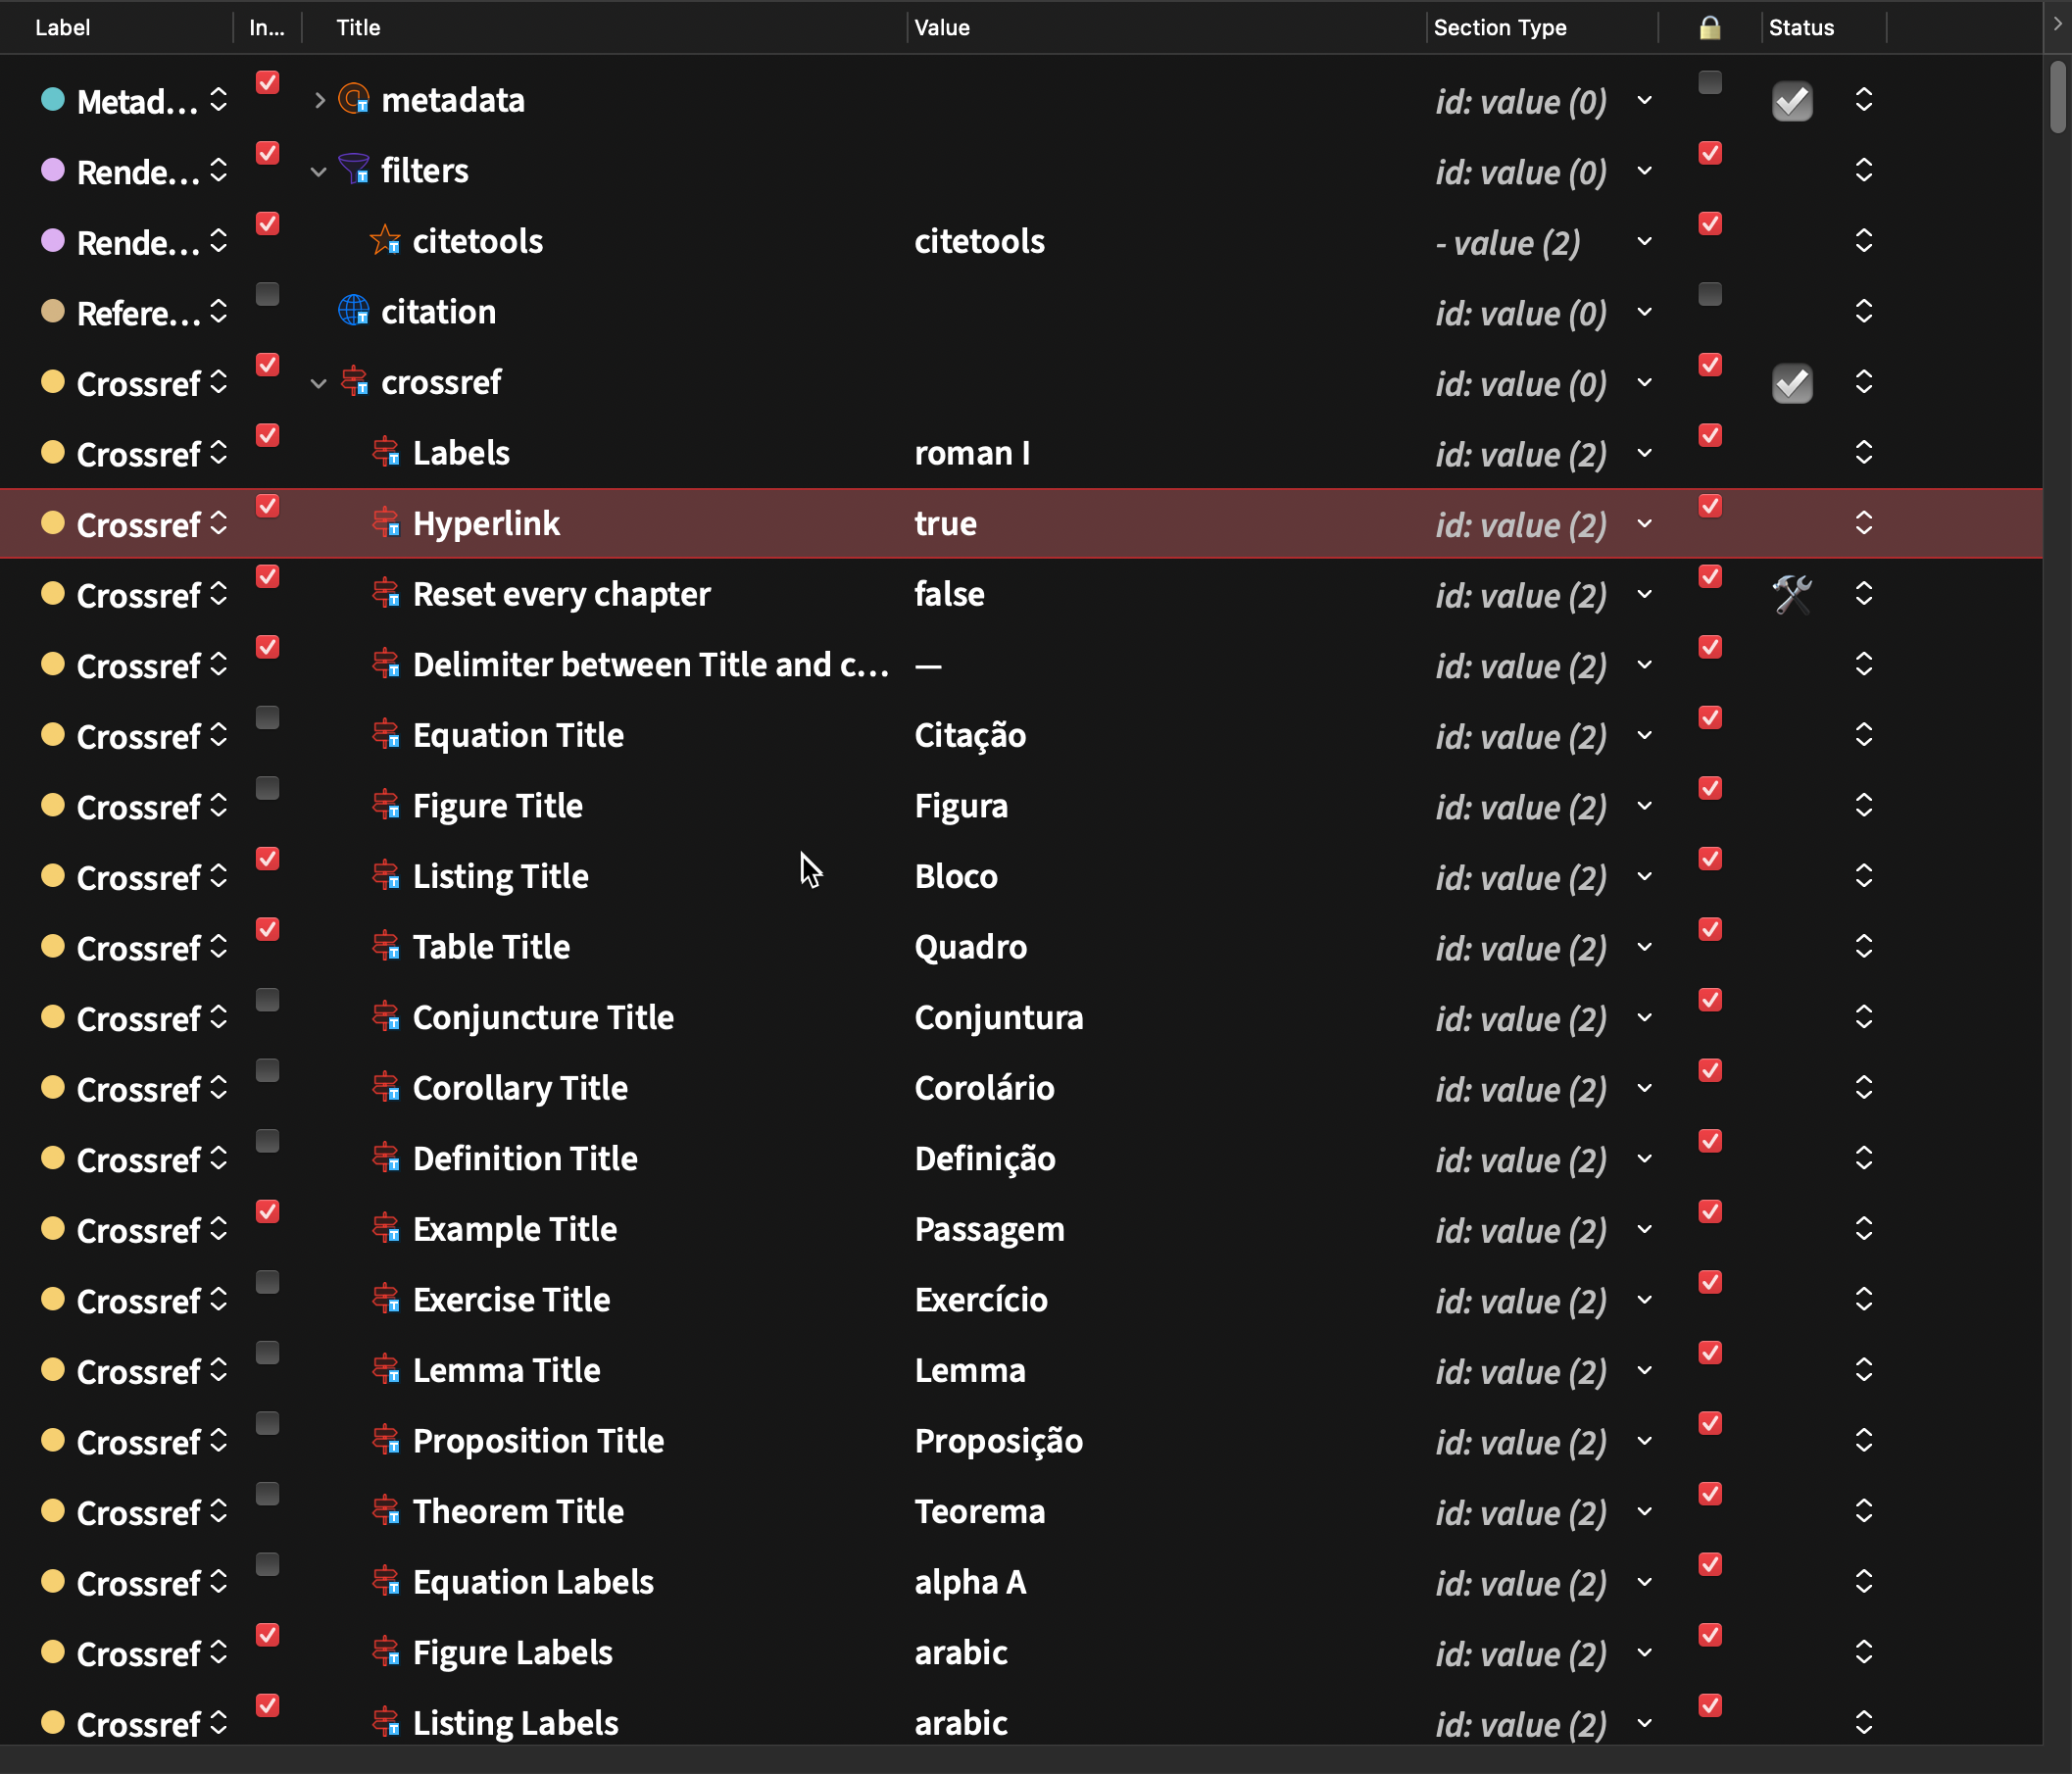
\includegraphics[width=5.20833in,height=4.36458in]{crossref.png}

}

\caption{\label{fig-scriv2A}Instead of using the \texttt{Title}, the
YAML key-value pair is usually formed by item's
\texttt{\textless{}\textbackslash{}\$custom:ID\textgreater{}}, and
\texttt{\textless{}\textbackslash{}\$custom:Value\textgreater{}} or
\texttt{Text} to allow the of more descriptive titles. The new front
matter also makes it a breeze to edit parameters without disturbing
YAML's sensitive white space rules, and it makes it much easier to
revert to a working configuration after introducing accidental errors.}

\end{figure}

\begin{figure}

{\centering 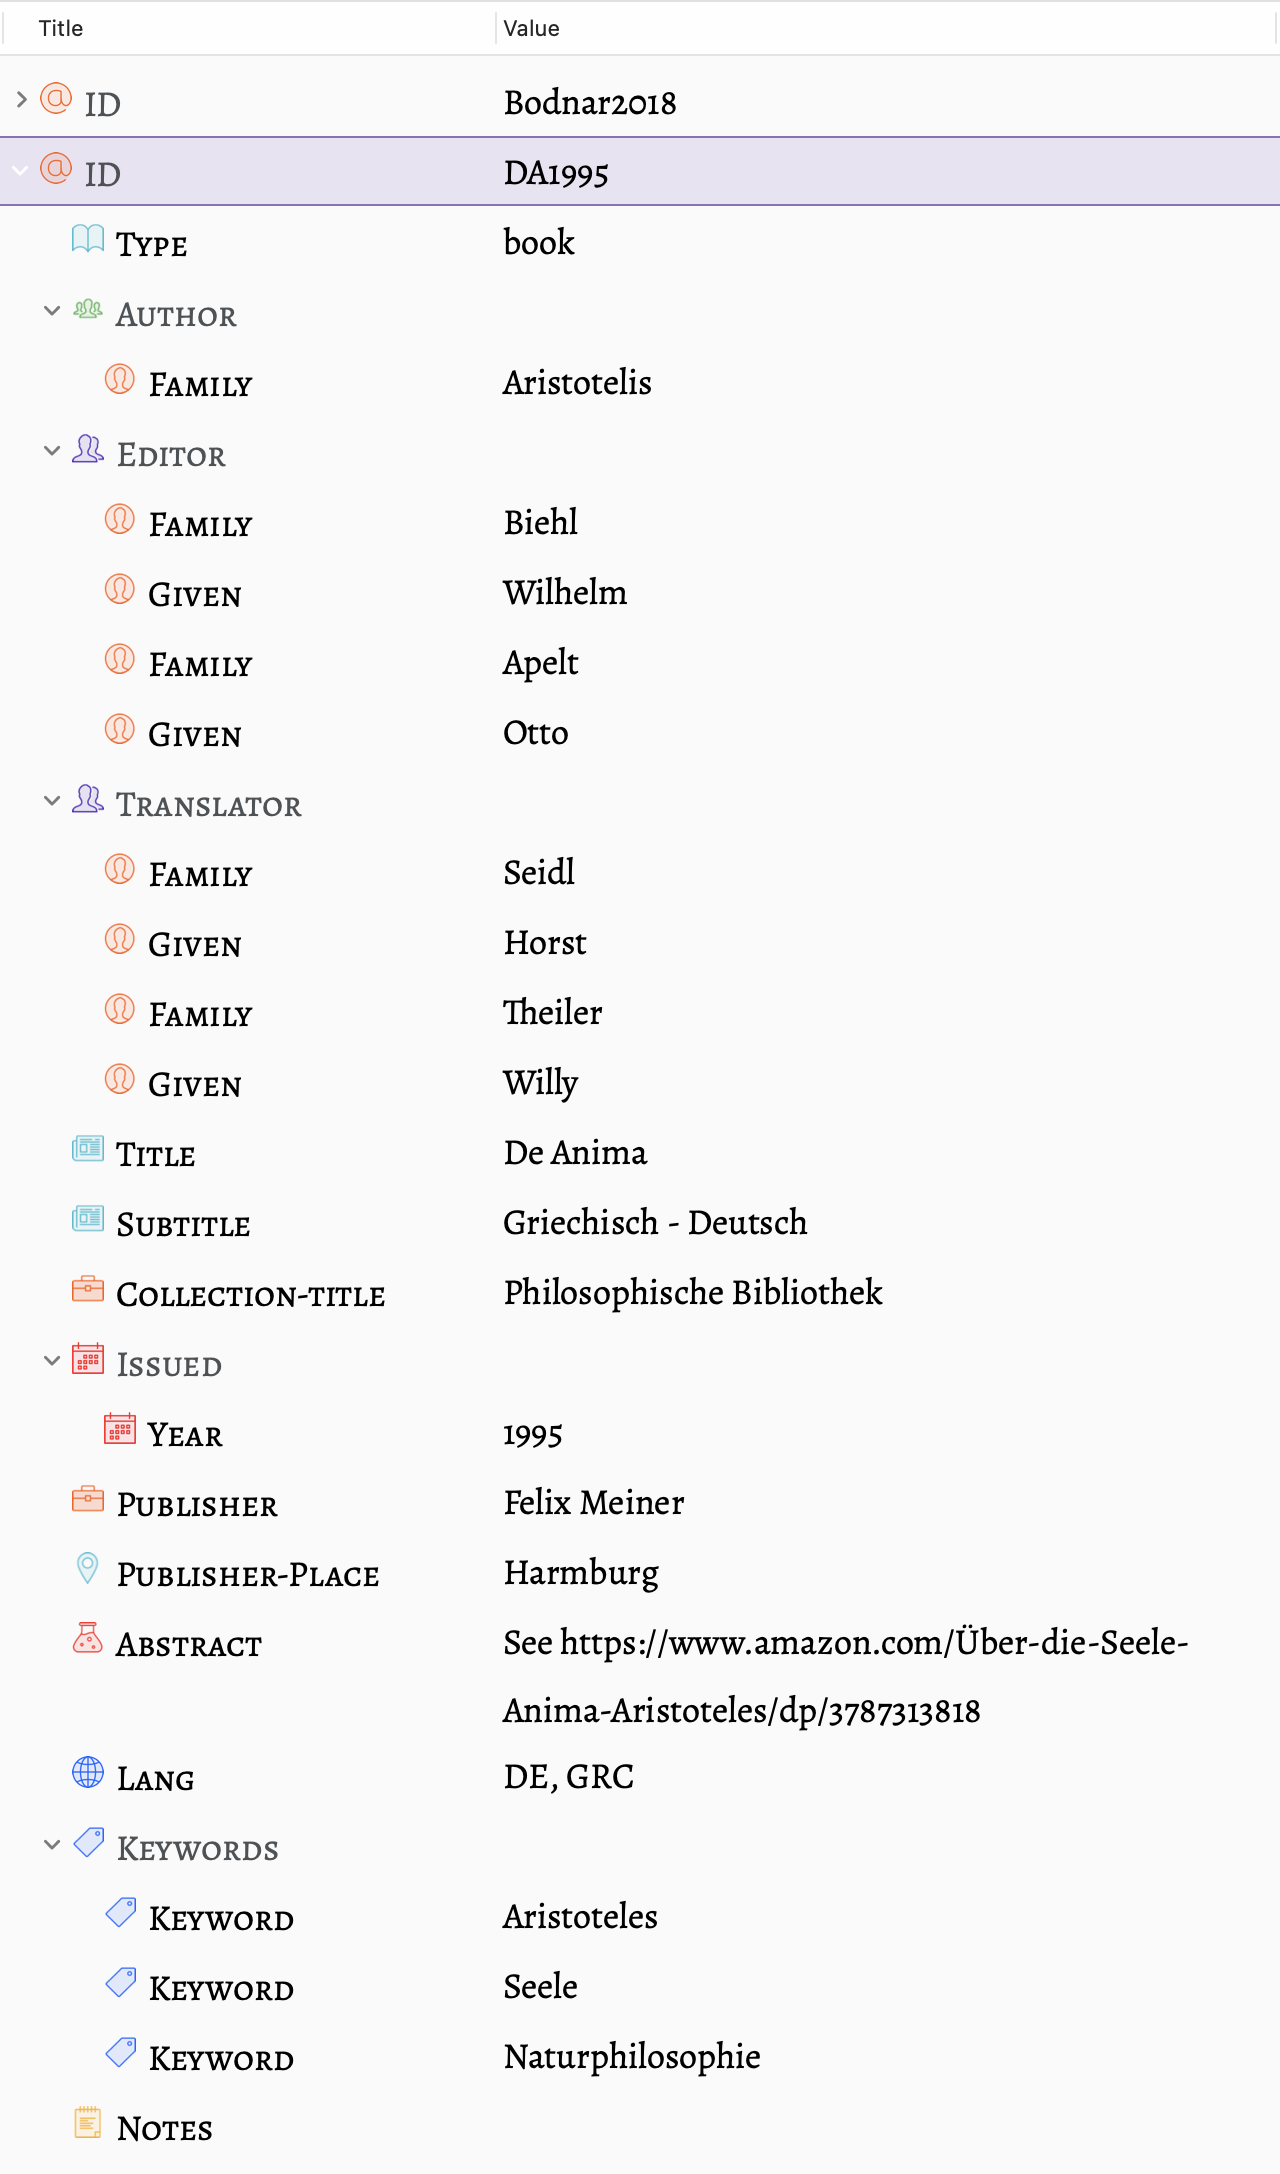
\includegraphics[width=3.66667in,height=6.25in]{cslyaml.png}

}

\caption{\label{fig-scriv2B}This demonstrates how to keep, entirely
within Scrivener, a bibliography in CSL-YAML, the format favored by
Pandoc and Quarto (being +10x faster to process than BibTeX and RIS).
You can find this sample in the templates folder.}

\end{figure}

\begin{tcolorbox}[enhanced jigsaw, rightrule=.15mm, bottomtitle=1mm, colback=white, toptitle=1mm, left=2mm, colbacktitle=quarto-callout-note-color!10!white, opacitybacktitle=0.6, opacityback=0, arc=.35mm, leftrule=.75mm, toprule=.15mm, titlerule=0mm, breakable, coltitle=black, bottomrule=.15mm, colframe=quarto-callout-note-color-frame, title=\textcolor{quarto-callout-note-color}{\faInfo}\hspace{0.5em}{A sworn of parameters}]

Many parameters are included for completeness and could be erased if
they are not in use. Should they become necessary, they can be retrieved
again from a newly created project.

\end{tcolorbox}

Looking for one way to control \textbf{Quarto} from \textbf{Scrivener},
we find not \emph{one}, but \emph{many} ways of doing so. So much that
we are reminded of Socrates addressing Meno, in the homonymous dialogue,
saying that, in looking for \emph{the} virtue of human excellence, he
had found a sworn of them coming from his interlocutor.

\begin{tcolorbox}[enhanced jigsaw, rightrule=.15mm, bottomtitle=1mm, colback=white, toptitle=1mm, left=2mm, colbacktitle=quarto-callout-caution-color!10!white, opacitybacktitle=0.6, opacityback=0, arc=.35mm, leftrule=.75mm, toprule=.15mm, titlerule=0mm, breakable, coltitle=black, bottomrule=.15mm, colframe=quarto-callout-caution-color-frame, title=\textcolor{quarto-callout-caution-color}{\faFire}\hspace{0.5em}{Binder glitches}]

In some cases, the sheer number of items can cause the \textbf{Binder}
to behave in strange ways. If you notice any glitches, collapse and
expand the parent item for the children to be properly displayed.
Removing unused parameters should alleviate the problem.

\end{tcolorbox}

Apart from one-click compilation, and facilitated parameter settings,
two priorities in \textbf{ScrivQ} are cross-referencing
(\protect\hypertarget{cite_4}{}{\label{cite_4}Section~\ref{sec-scriv3}})
and bibliography
(\protect\hypertarget{cite_5}{}{\label{cite_5}Section~\ref{sec-scriv41}}).

\hypertarget{sec-scriv3}{%
\chapter{Cross-referencing}\label{sec-scriv3}}

With all the affordances of \textbf{Scrivener} and \textbf{Quarto},
cross-referencing is not a trivial matter, \ul{as the options are many}.

{\marginnote{\begin{footnotesize}Automatic IDs\end{footnotesize}}}First,
bear in mind that \textbf{Section Types} and \textbf{Paragraph Styles}
are rigged with automatic IDs in the format
\ul{scriv\textless\$linkID\textgreater{}}\footnote{Note that in
  Scrivener we have to escape the \texttt{\$}, otherwise the placeholder
  will get expanded into its correct value during compilation.}
(preceded by the relevant prefix, such as \emph{sec}, \emph{cnj},
\emph{cor}, \emph{def}, \emph{exm}, \emph{exr}, \emph{lem}, \emph{prp},
\emph{thm}, \emph{eq}, \emph{lst}, \emph{fig}, \emph{tbl}) . This way,
there is no need to choose an ID each time an element is created, nor to
remember any when another needs to be referenced (to create links we
will use this same standard identifier,
\ul{scriv\textless\$linkID\textgreater{}}, select the text, link to the
appropriate document, and apply the style corresponding to the element
we want to reference). We leave it to Scrivener to figure out the value
of the \ul{\textless\$linkID\textgreater{}} placeholder.

\begin{tcolorbox}[enhanced jigsaw, rightrule=.15mm, bottomtitle=1mm, colback=white, toptitle=1mm, left=2mm, colbacktitle=quarto-callout-note-color!10!white, opacitybacktitle=0.6, opacityback=0, arc=.35mm, leftrule=.75mm, toprule=.15mm, titlerule=0mm, breakable, coltitle=black, bottomrule=.15mm, colframe=quarto-callout-note-color-frame, title=\textcolor{quarto-callout-note-color}{\faInfo}\hspace{0.5em}{Translating Quarto into Scrivener}]

In \textbf{ScrivQ} we can use \textbf{Section Types} or
\textbf{Paragraph Styles} to create \textbf{Sections}, \textbf{Tables},
\textbf{Equations}, \textbf{Figures}, \textbf{Listings},
\textbf{Callouts} (Caution, Important, Note, Tip, Warning), and
\textbf{Amsthm} environments (Conjecture, Corollary, Definition,
Example, Exercise, Lemma, Proposition, Theorem). We can also use
\textbf{Character Styles} to easily reference any of them. Keep reading
to learn how.

\end{tcolorbox}

\begin{tcolorbox}[enhanced jigsaw, rightrule=.15mm, bottomtitle=1mm, colback=white, toptitle=1mm, left=2mm, colbacktitle=quarto-callout-tip-color!10!white, opacitybacktitle=0.6, opacityback=0, arc=.35mm, leftrule=.75mm, toprule=.15mm, titlerule=0mm, breakable, coltitle=black, bottomrule=.15mm, colframe=quarto-callout-tip-color-frame, title=\textcolor{quarto-callout-tip-color}{\faLightbulb}\hspace{0.5em}{Choosing your own label for automatic links}]

In \textbf{ScrivQ} one can use different keywords as labels for
automatic links. Simply use one of the provided rules for
\textbf{Replacements}
(\protect\hypertarget{cite_6}{}{\label{cite_6}Figure~\ref{fig-scriv3}})
in the Compile settings (or in the Format configurations) to have
keywords such as \ul{scriv} + \ul{link}, \ul{autο} + \ul{ref},
\ul{\%autο} + \ul{ref\%}, \ul{\%autοref:} +
\ul{something-random-that-will-be-erased\%}, \ul{{[}autοref{]}},
converted into \ul{scriv\textless\$linkID\textgreater{}} during
compilation.

\end{tcolorbox}

\begin{figure}

{\centering 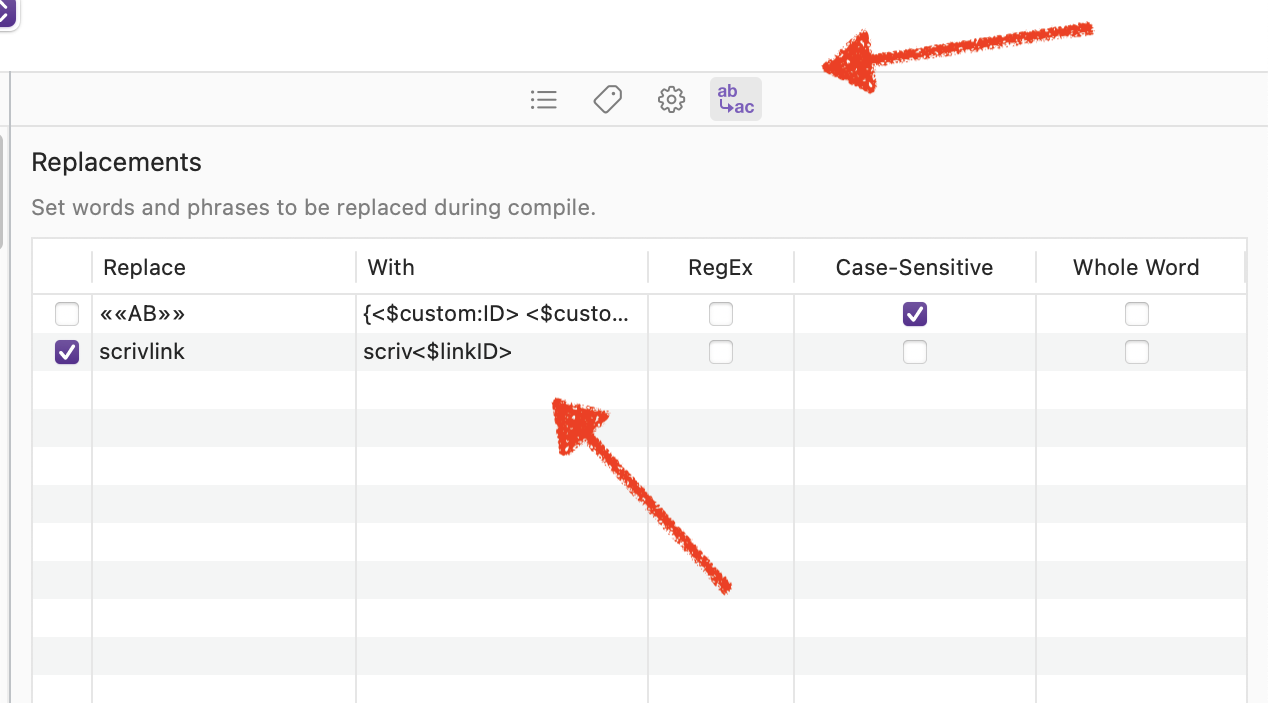
\includegraphics[width=4.30208in,height=2.38542in]{Replacements.png}

}

\caption{\label{fig-scriv3}\textbf{Replacements} pane in the
\textbf{Compile\ldots{}} configurations can be used to allow different
labels for automatic links. This is purely optional and we recommend
limiting this to one rule or two.}

\end{figure}

{\marginnote{\begin{footnotesize}Add prefix and markup using Character
Styles\end{footnotesize}}}To cross-reference a \textbf{table}, an
\textbf{example}, or a \textbf{theorem}, one could use \ul{tbl-keyword}
(\emph{i.e.} \ul{tbl-scriv\textless\$linkID\textgreater{}}),
\ul{exm-keyword} (\emph{i.e.}
\ul{exm-scriv\textless\$linkID\textgreater{}}), and \ul{thm-keyword}
(\emph{i.e.} \ul{thm-scriv\textless\$linkID\textgreater{}}),
respectively. Seeing that the prefixes are not always easy to remember,
\textbf{Character Styles} are available to inject the correct markup.

The \emph{Crossref Table}, for example, will turn the \ul{keyword} into
\ul{{[}@tbl-keyword{]}}\footnote{That is,
  \texttt{{[}@tbl-scriv\textless{}\textbackslash{}\$linkID\textgreater{}{]}}.}\ul{;}
and th\emph{e Crossref Table*} style will turn it into
\ul{\protect\hypertarget{cite_7}{}{\label{cite_7}\textbf{?@tbl-keyword}}}\footnote{That
  is,
  \texttt{{[}-@tbl-scriv\textless{}\textbackslash{}\$linkID\textgreater{}{]}}.}.
{\marginnote{\begin{footnotesize}The asterisk (\texttt{*}) in the title
of Character Styles indicates the suppression of part of the data (as is
common in LaTeX).\end{footnotesize}}} Likewise, the \emph{Crossref
Example} and the \emph{Crossref Example*} will result in
\ul{{[}@exm-keyword{]}} and \ul{{[}-@exm-keyword{]}}\footnote{That is,
  \texttt{{[}@exm-scriv\textless{}\textbackslash{}\$linkID\textgreater{}{]}}
  and
  \texttt{{[}-@exm-scriv\textless{}\textbackslash{}\$linkID\textgreater{}{]}}.},
and so on. See \emph{scriv4} below for yet more examples.

\begin{tcolorbox}[enhanced jigsaw, rightrule=.15mm, bottomtitle=1mm, colback=white, toptitle=1mm, left=2mm, colbacktitle=quarto-callout-tip-color!10!white, opacitybacktitle=0.6, opacityback=0, arc=.35mm, leftrule=.75mm, toprule=.15mm, titlerule=0mm, breakable, coltitle=black, bottomrule=.15mm, colframe=quarto-callout-tip-color-frame, title=\textcolor{quarto-callout-tip-color}{\faLightbulb}\hspace{0.5em}{Cross-referencing a table}]

\begin{enumerate}
\def\labelenumi{\arabic{enumi}.}
\tightlist
\item
  Type \ul{your-keyword-of-choice} or
  \ul{scriv\textless\$linkID\textgreater{}}, select it, and hit
  \ul{Command + L};
\item
  Link to the document that contains the table.
\item
  Apply a \textbf{Character Style} called \emph{Crossref Table} (e.g.
  \protect\hypertarget{cite_8}{}{\label{cite_8}Table~\ref{tbl-scriv3}}).
\end{enumerate}

\end{tcolorbox}

Below we will see several examples of the same strategy being applied to
several different elements. I hope that these examples prove as
instructive to consult as they were to prepare.

\hypertarget{tbl-scriv3}{}
\begin{longtable}[]{@{}cccc@{}}
\toprule\noalign{}
\textbf{Genus} & \textbf{Species} & \textbf{Markdown Source} &
\textbf{Rendered Output} \\
\midrule\noalign{}
\endfirsthead
\toprule\noalign{}
\textbf{Genus} & \textbf{Species} & \textbf{Markdown Source} &
\textbf{Rendered Output} \\
\midrule\noalign{}
\endhead
\bottomrule\noalign{}
\endlastfoot
Amsthm & Conjecture & \texttt{{[}@cnj-scriv4{]}} &
\protect\hypertarget{cite_9}{}{\label{cite_9}Conjecture~\ref{cnj-scriv4}} \\
Amsthm & Conjecture & \texttt{{[}@cnj-scriv5{]}} &
\protect\hypertarget{cite_10}{}{\label{cite_10}Conjecture~\ref{cnj-scriv5}} \\
Amsthm & Corollary & \texttt{{[}@cor-scriv4{]}} &
\protect\hypertarget{cite_11}{}{\label{cite_11}Corollary~\ref{cor-scriv4}} \\
Amsthm & Corollary & \texttt{{[}@cor-scriv6{]}} &
\protect\hypertarget{cite_12}{}{\label{cite_12}Corollary~\ref{cor-scriv6}} \\
Amsthm & Definition & \texttt{{[}@def-scriv4{]}} &
\protect\hypertarget{cite_13}{}{\label{cite_13}Definition~\ref{def-scriv4}} \\
Amsthm & Definition & \texttt{{[}@def-scriv7{]}} &
\protect\hypertarget{cite_14}{}{\label{cite_14}Definition~\ref{def-scriv7}} \\
Amsthm & Example & \texttt{{[}@exm-scriv4{]}} &
\protect\hypertarget{cite_15}{}{\label{cite_15}Example~\ref{exm-scriv4}} \\
Amsthm & Example & \texttt{{[}@exm-scriv8{]}} &
\protect\hypertarget{cite_16}{}{\label{cite_16}Example~\ref{exm-scriv8}} \\
Amsthm & Exercise & \texttt{{[}@exr-scriv4{]}} &
\protect\hypertarget{cite_17}{}{\label{cite_17}Exercise~\ref{exr-scriv4}} \\
Amsthm & Exercise & \texttt{{[}@exr-scriv9{]}} &
\protect\hypertarget{cite_18}{}{\label{cite_18}Exercise~\ref{exr-scriv9}} \\
Amsthm & Lemma & \texttt{{[}@lem-scriv4{]}} &
\protect\hypertarget{cite_19}{}{\label{cite_19}Lemma~\ref{lem-scriv4}} \\
Amsthm & Lemma & \texttt{{[}@lem-scriv10{]}} &
\protect\hypertarget{cite_20}{}{\label{cite_20}Lemma~\ref{lem-scriv10}} \\
Amsthm & Proposition & \texttt{{[}@prp-scriv4{]}} &
\protect\hypertarget{cite_21}{}{\label{cite_21}Proposition~\ref{prp-scriv4}} \\
Amsthm & Proposition & \texttt{{[}@prp-scriv11{]}} &
\protect\hypertarget{cite_22}{}{\label{cite_22}Proposition~\ref{prp-scriv11}} \\
Amsthm & Theorem & \texttt{{[}@thm-scriv4{]}} &
\protect\hypertarget{cite_23}{}{\label{cite_23}Theorem~\ref{thm-scriv4}} \\
Amsthm & Theorem & \texttt{{[}@thm-scriv12{]}} &
\protect\hypertarget{cite_24}{}{\label{cite_24}Theorem~\ref{thm-scriv12}} \\
Diagram & Dot & \texttt{{[}@fig-scriv14{]}} &
\protect\hypertarget{cite_25}{}{\label{cite_25}Figure~\ref{fig-scriv14}} \\
Diagram & Dot & \texttt{{[}@fig-scriv14B{]}} &
\protect\hypertarget{cite_26}{}{\label{cite_26}Figure~\ref{fig-scriv14B}} \\
Diagram & Dot & \texttt{{[}@fig-scriv15{]}} &
\protect\hypertarget{cite_27}{}{\label{cite_27}Figure~\ref{fig-scriv15}} \\
Diagram & Mermaid & \texttt{{[}@fig-scriv16{]}} &
\protect\hypertarget{cite_28}{}{\label{cite_28}Figure~\ref{fig-scriv16}} \\
Diagram & Mermaid & \texttt{{[}@fig-scriv16B{]}} &
\protect\hypertarget{cite_29}{}{\label{cite_29}Figure~\ref{fig-scriv16B}} \\
Diagram & Mermaid & \texttt{{[}@fig-scriv17{]}} &
\protect\hypertarget{cite_30}{}{\label{cite_30}Figure~\ref{fig-scriv17}} \\
Cross-reference & Equation & \texttt{{[}@eq-scriv19{]}} &
\protect\hypertarget{cite_31}{}{\label{cite_31}Equation~\ref{eq-scriv19}} \\
Cross-reference & Equation & \texttt{{[}@eq-scriv20{]}} &
\protect\hypertarget{cite_32}{}{\label{cite_32}Equation~\ref{eq-scriv20}} \\
Cross-reference & Figure & \texttt{{[}@fig-scriv22{]}} &
\protect\hypertarget{cite_33}{}{\label{cite_33}Figure~\ref{fig-scriv22}} \\
Cross-reference & Listing & \texttt{{[}@lst-scriv26{]}} &
\protect\hypertarget{cite_34}{}{\label{cite_34}Listing~\ref{lst-scriv26}} \\
Cross-reference & Listing & \texttt{{[}@lst-scriv27{]}} &
\protect\hypertarget{cite_35}{}{\label{cite_35}Listing~\ref{lst-scriv27}} \\
Cross-reference & Table & \texttt{{[}@tbl-scriv30{]}} &
\protect\hypertarget{cite_36}{}{\label{cite_36}Table~\ref{tbl-scriv30}} \\
Cross-reference & Table & \texttt{{[}@tbl-scriv31{]}} &
\protect\hypertarget{cite_37}{}{\label{cite_37}Table~\ref{tbl-scriv31}} \\
Cross-reference & Section & \texttt{{[}@sec-scriv33{]}} &
\protect\hypertarget{cite_38}{}{\label{cite_38}Section~\ref{sec-scriv33}} \\
Cross-reference & Section & \texttt{{[}@sec-scriv34{]}} &
\protect\hypertarget{cite_39}{}{\label{cite_39}Section~\ref{sec-scriv34}} \\
Cross-reference & Section & \texttt{{[}@sec-scriv36{]}} &
\protect\hypertarget{cite_40}{}{\label{cite_40}Section~\ref{sec-scriv36}} \\
Cross-reference & Section & \texttt{{[}@sec-scriv38{]}} &
\protect\hypertarget{cite_41}{}{\label{cite_41}Section~\ref{sec-scriv38}} \\
Multipart & Figure & \texttt{{[}@fig-scriv23{]}} &
\protect\hypertarget{cite_42}{}{\label{cite_42}Figure~\ref{fig-scriv23}} \\
Multipart & Figure & \texttt{{[}@fig-scriv23A{]}} &
\protect\hypertarget{cite_43}{}{\label{cite_43}Figure~\ref{fig-scriv23A}} \\
Multipart & Figure & \texttt{{[}@fig-scriv23B{]}} &
\protect\hypertarget{cite_44}{}{\label{cite_44}Figure~\ref{fig-scriv23B}} \\
Multipart & Figure & \texttt{{[}@fig-scriv24{]}} &
\protect\hypertarget{cite_45}{}{\label{cite_45}Figure~\ref{fig-scriv24}} \\
Multipart & Figure & \texttt{{[}@fig-scriv24A{]}} &
\protect\hypertarget{cite_46}{}{\label{cite_46}Figure~\ref{fig-scriv24A}} \\
Multipart & Figure & \texttt{{[}@fig-scriv24B{]}} &
\protect\hypertarget{cite_47}{}{\label{cite_47}Figure~\ref{fig-scriv24B}} \\
Multipart & Table & \texttt{{[}@tbl-scriv32{]}} &
\protect\hypertarget{cite_48}{}{\label{cite_48}Table~\ref{tbl-scriv32}} \\
Multipart & Table & \texttt{{[}@tbl-scriv32A{]}} &
\protect\hypertarget{cite_49}{}{\label{cite_49}Table~\ref{tbl-scriv32A}} \\
Multipart & Table & \texttt{{[}@tbl-scriv32B{]}} &
\protect\hypertarget{cite_50}{}{\label{cite_50}Table~\ref{tbl-scriv32B}} \\
\caption{\label{tbl-scriv3}Cross-referencing amsthm theorems, diagrams,
figures, listings, tables, and sections.}\tabularnewline
\end{longtable}

\newpage{}

\hypertarget{sec-scriv4}{%
\section{Amsthm}\label{sec-scriv4}}

In this section, we are demonstrating the cross-referencing mechanism
working with \textbf{Amsthm} theorems. First, we will see all of the
theorems created using \textbf{Paragraph Styles}, then they will be
introduced again as \textbf{Section Types}. In the table below, you'll
see several Character Styles (labeled as \ul{Crossref\ldots{}}) used to
reference both.

\hypertarget{tbl-scriv4}{}
\begin{longtable}[]{@{}ccc@{}}
\toprule\noalign{}
\textbf{Element} & \textbf{Markdown Source} & \textbf{Rendered
Output} \\
\midrule\noalign{}
\endfirsthead
\toprule\noalign{}
\textbf{Element} & \textbf{Markdown Source} & \textbf{Rendered
Output} \\
\midrule\noalign{}
\endhead
\bottomrule\noalign{}
\endlastfoot
Conjecture & \texttt{{[}@cnj-scriv4{]}} &
\protect\hypertarget{cite_51}{}{\label{cite_51}Conjecture~\ref{cnj-scriv4}} \\
Conjecture & \texttt{{[}@cnj-scriv5{]}} &
\protect\hypertarget{cite_52}{}{\label{cite_52}Conjecture~\ref{cnj-scriv5}} \\
Corollary & \texttt{{[}@cor-scriv4{]}} &
\protect\hypertarget{cite_53}{}{\label{cite_53}Corollary~\ref{cor-scriv4}} \\
Corollary & \texttt{{[}@cor-scriv6{]}} &
\protect\hypertarget{cite_54}{}{\label{cite_54}Corollary~\ref{cor-scriv6}} \\
Definition & \texttt{{[}@def-scriv4{]}} &
\protect\hypertarget{cite_55}{}{\label{cite_55}Definition~\ref{def-scriv4}} \\
Definition & \texttt{{[}@def-scriv7{]}} &
\protect\hypertarget{cite_56}{}{\label{cite_56}Definition~\ref{def-scriv7}} \\
Example & \texttt{{[}@exm-scriv4{]}} &
\protect\hypertarget{cite_57}{}{\label{cite_57}Example~\ref{exm-scriv4}} \\
Example & \texttt{{[}@exm-scriv8{]}} &
\protect\hypertarget{cite_58}{}{\label{cite_58}Example~\ref{exm-scriv8}} \\
Exercise & \texttt{{[}@exr-scriv4{]}} &
\protect\hypertarget{cite_59}{}{\label{cite_59}Exercise~\ref{exr-scriv4}} \\
Exercise & \texttt{{[}@exr-scriv9{]}} &
\protect\hypertarget{cite_60}{}{\label{cite_60}Exercise~\ref{exr-scriv9}} \\
Lemma & \texttt{{[}@lem-scriv4{]}} &
\protect\hypertarget{cite_61}{}{\label{cite_61}Lemma~\ref{lem-scriv4}} \\
Lemma & \texttt{{[}@lem-scriv10{]}} &
\protect\hypertarget{cite_62}{}{\label{cite_62}Lemma~\ref{lem-scriv10}} \\
Proposition & \texttt{{[}@prp-scriv4{]}} &
\protect\hypertarget{cite_63}{}{\label{cite_63}Proposition~\ref{prp-scriv4}} \\
Proposition & \texttt{{[}@prp-scriv11{]}} &
\protect\hypertarget{cite_64}{}{\label{cite_64}Proposition~\ref{prp-scriv11}} \\
Theorem & \texttt{{[}@thm-scriv4{]}} &
\protect\hypertarget{cite_65}{}{\label{cite_65}Theorem~\ref{thm-scriv4}} \\
Theorem & \texttt{{[}@thm-scriv12{]}} &
\protect\hypertarget{cite_66}{}{\label{cite_66}Theorem~\ref{thm-scriv12}} \\
\caption{\label{tbl-scriv4}Cross-referencing amsthm elements in
ScrivQ.}\tabularnewline
\end{longtable}

\textbf{Paragraph Styles}

\begin{conjecture}[]\protect\hypertarget{cnj-scriv4}{}\label{cnj-scriv4}

Conjecture

\end{conjecture}

\begin{corollary}[]\protect\hypertarget{cor-scriv4}{}\label{cor-scriv4}

Corollary

\end{corollary}

\begin{definition}[]\protect\hypertarget{def-scriv4}{}\label{def-scriv4}

Definition

\end{definition}

\begin{example}[]\protect\hypertarget{exm-scriv4}{}\label{exm-scriv4}

Example

\end{example}

\begin{exercise}[]\protect\hypertarget{exr-scriv4}{}\label{exr-scriv4}

Exercise

\end{exercise}

\begin{lemma}[]\protect\hypertarget{lem-scriv4}{}\label{lem-scriv4}

Lemma

\end{lemma}

\begin{proposition}[]\protect\hypertarget{prp-scriv4}{}\label{prp-scriv4}

Proposition

\end{proposition}

\begin{theorem}[Pythagorean
theorem]\protect\hypertarget{thm-scriv4}{}\label{thm-scriv4}

\[[ x^2 + y^2 = z^2 ]\]

\end{theorem}

\textbf{Section Types}

\begin{conjecture}[]\protect\hypertarget{cnj-scriv5}{}\label{cnj-scriv5}

Conjecture

\end{conjecture}

\begin{corollary}[]\protect\hypertarget{cor-scriv6}{}\label{cor-scriv6}

Corollary

\end{corollary}

\begin{definition}[]\protect\hypertarget{def-scriv7}{}\label{def-scriv7}

Definition

\end{definition}

\begin{example}[]\protect\hypertarget{exm-scriv8}{}\label{exm-scriv8}

Example

\end{example}

\begin{exercise}[]\protect\hypertarget{exr-scriv9}{}\label{exr-scriv9}

Exercise

\end{exercise}

\begin{lemma}[]\protect\hypertarget{lem-scriv10}{}\label{lem-scriv10}

Lemma

\end{lemma}

\begin{proposition}[]\protect\hypertarget{prp-scriv11}{}\label{prp-scriv11}

Proposition

\end{proposition}

\begin{theorem}[Pythagorean
theorem]\protect\hypertarget{thm-scriv12}{}\label{thm-scriv12}

~

\begin{theorem}[]\protect\hypertarget{thm-scriv12}{}\label{thm-scriv12}

\[[ x^2 + y^2 = z^2 ]\]

\end{theorem}

\end{theorem}

\newpage{}

\hypertarget{sec-scriv13}{%
\section{Diagrams}\label{sec-scriv13}}

Let us see how we can use \textbf{raw markup}, \textbf{Section Types},
and \textbf{Paragraph Styles} to create \textbf{Dot} and
\textbf{Mermaid} diagrams.

\hypertarget{tbl-scriv13}{}
\begin{longtable}[]{@{}ccc@{}}
\toprule\noalign{}
\textbf{Element} & \textbf{Markdown Source} & \textbf{Rendered
Output} \\
\midrule\noalign{}
\endfirsthead
\toprule\noalign{}
\textbf{Element} & \textbf{Markdown Source} & \textbf{Rendered
Output} \\
\midrule\noalign{}
\endhead
\bottomrule\noalign{}
\endlastfoot
Diagram Dot & \texttt{{[}@fig-scriv14{]}} &
\protect\hypertarget{cite_67}{}{\label{cite_67}Figure~\ref{fig-scriv14}} \\
Diagram Dot & \texttt{{[}@fig-scriv14B{]}} &
\protect\hypertarget{cite_68}{}{\label{cite_68}Figure~\ref{fig-scriv14B}} \\
Diagram Dot & \texttt{{[}@fig-scriv15{]}} &
\protect\hypertarget{cite_69}{}{\label{cite_69}Figure~\ref{fig-scriv15}} \\
Diagram Mermaid & \texttt{{[}@fig-scriv16{]}} &
\protect\hypertarget{cite_70}{}{\label{cite_70}Figure~\ref{fig-scriv16}} \\
Diagram Mermaid & \texttt{{[}@fig-scriv16B{]}} &
\protect\hypertarget{cite_71}{}{\label{cite_71}Figure~\ref{fig-scriv16B}} \\
Diagram Mermaid & \texttt{{[}@fig-scriv17{]}} &
\protect\hypertarget{cite_72}{}{\label{cite_72}Figure~\ref{fig-scriv17}} \\
\caption{\label{tbl-scriv13}Cross-referencing Dot and Mermaid
diagrams.}\tabularnewline
\end{longtable}

\begin{figure}

{\centering 

\begin{figure}[H]

{\centering 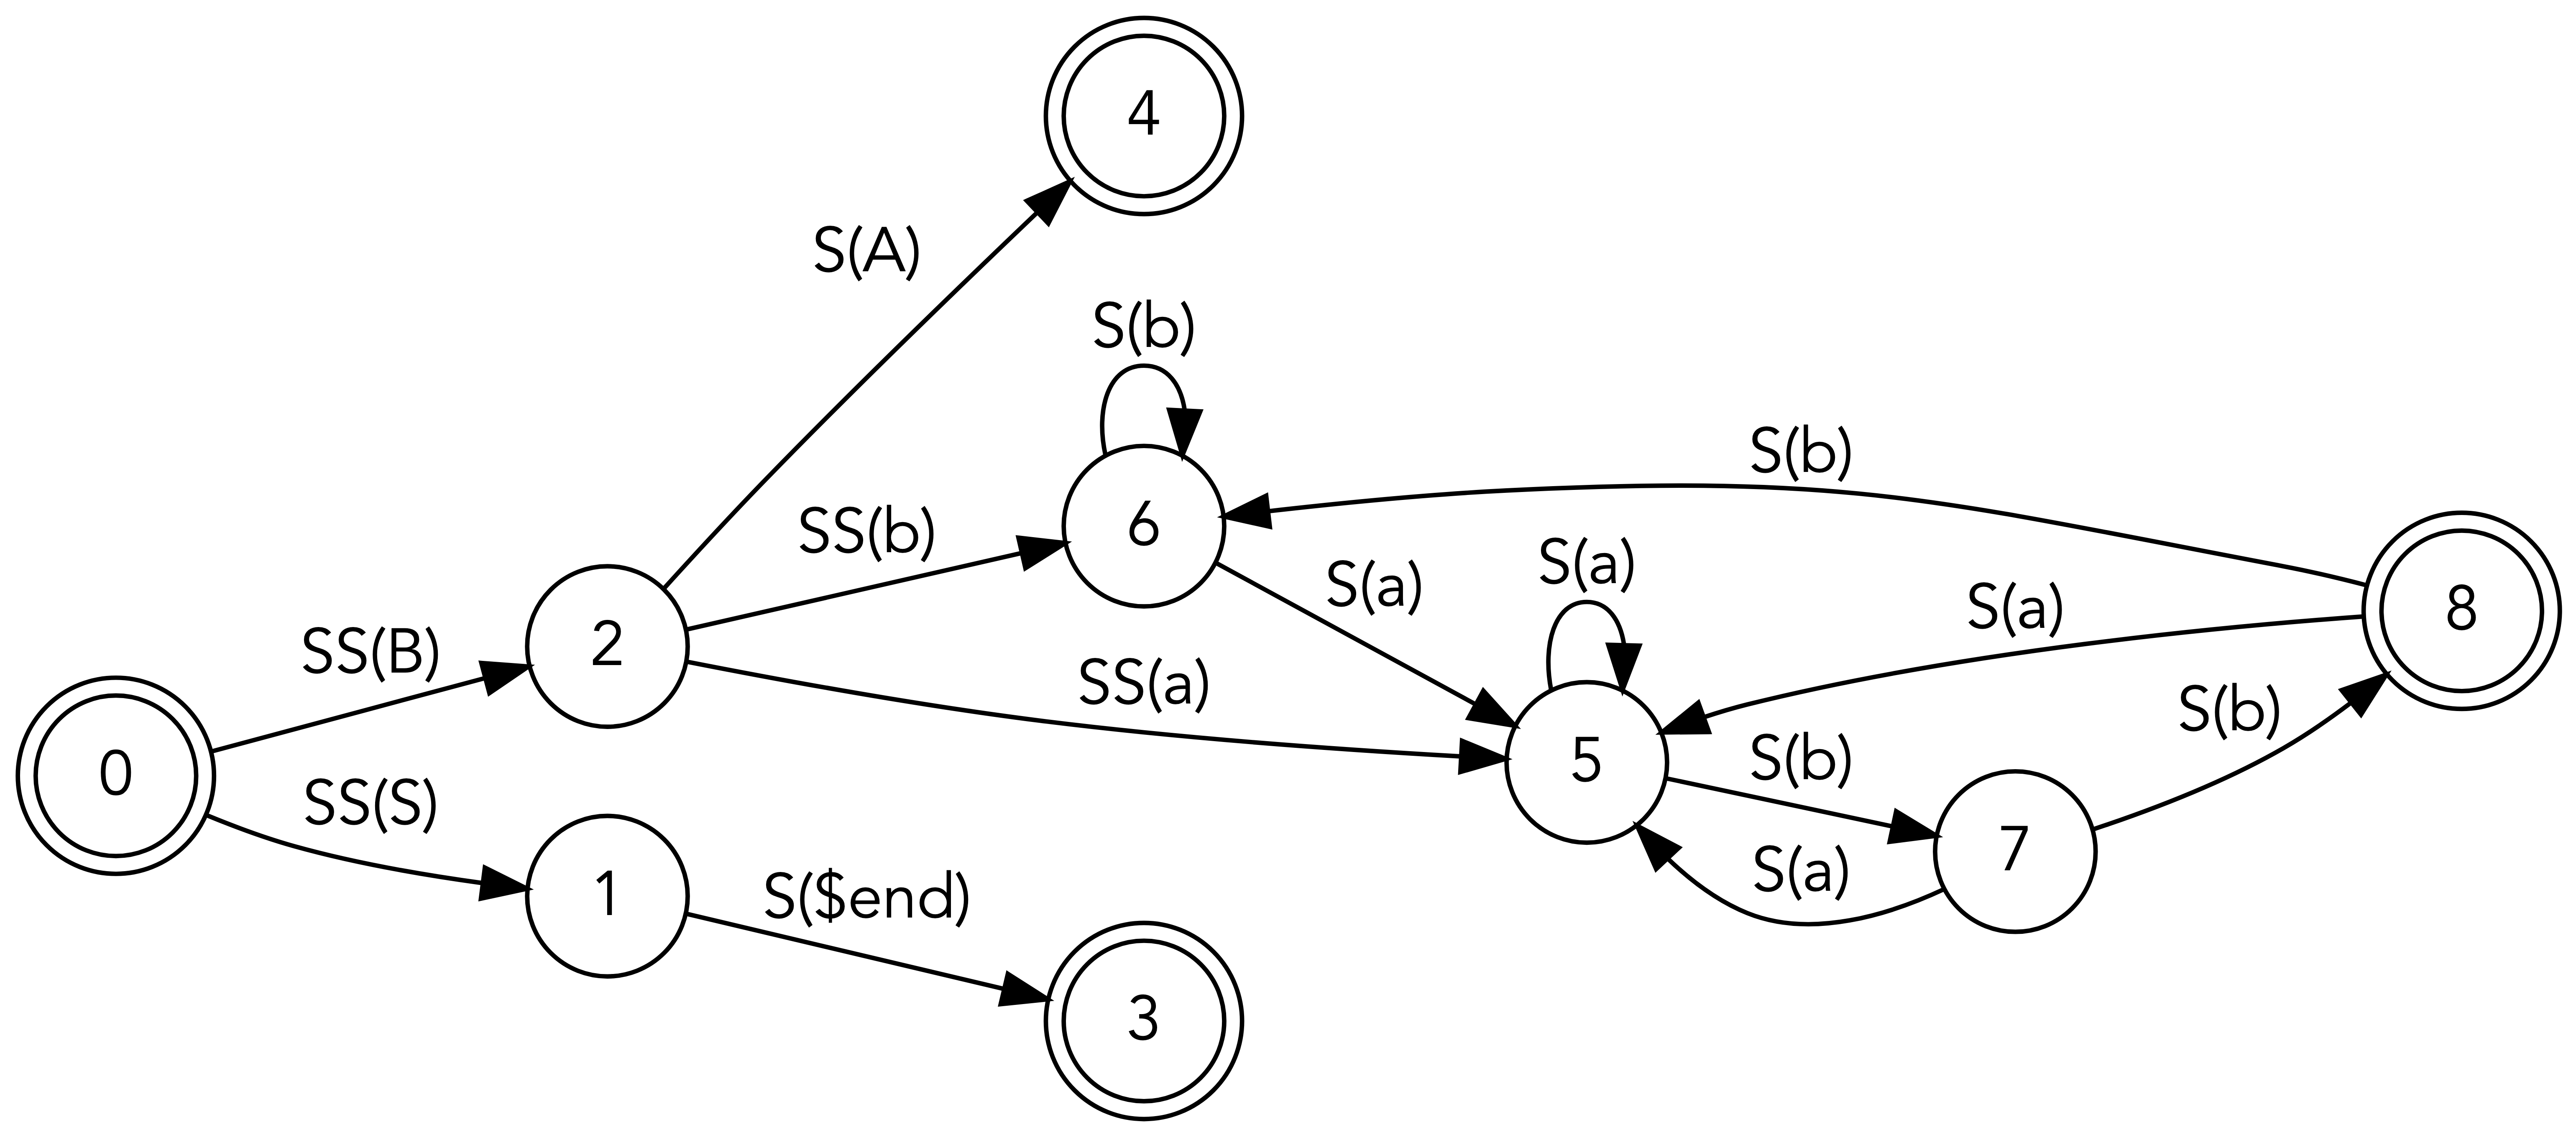
\includegraphics[width=5.5in,height=3.5in]{index_files/figure-latex/dot-figure-1.png}

}

\end{figure}

}

\caption{\label{fig-scriv14}Figure caption}

\end{figure}

\begin{figure}

{\centering 

\begin{figure}[H]

{\centering 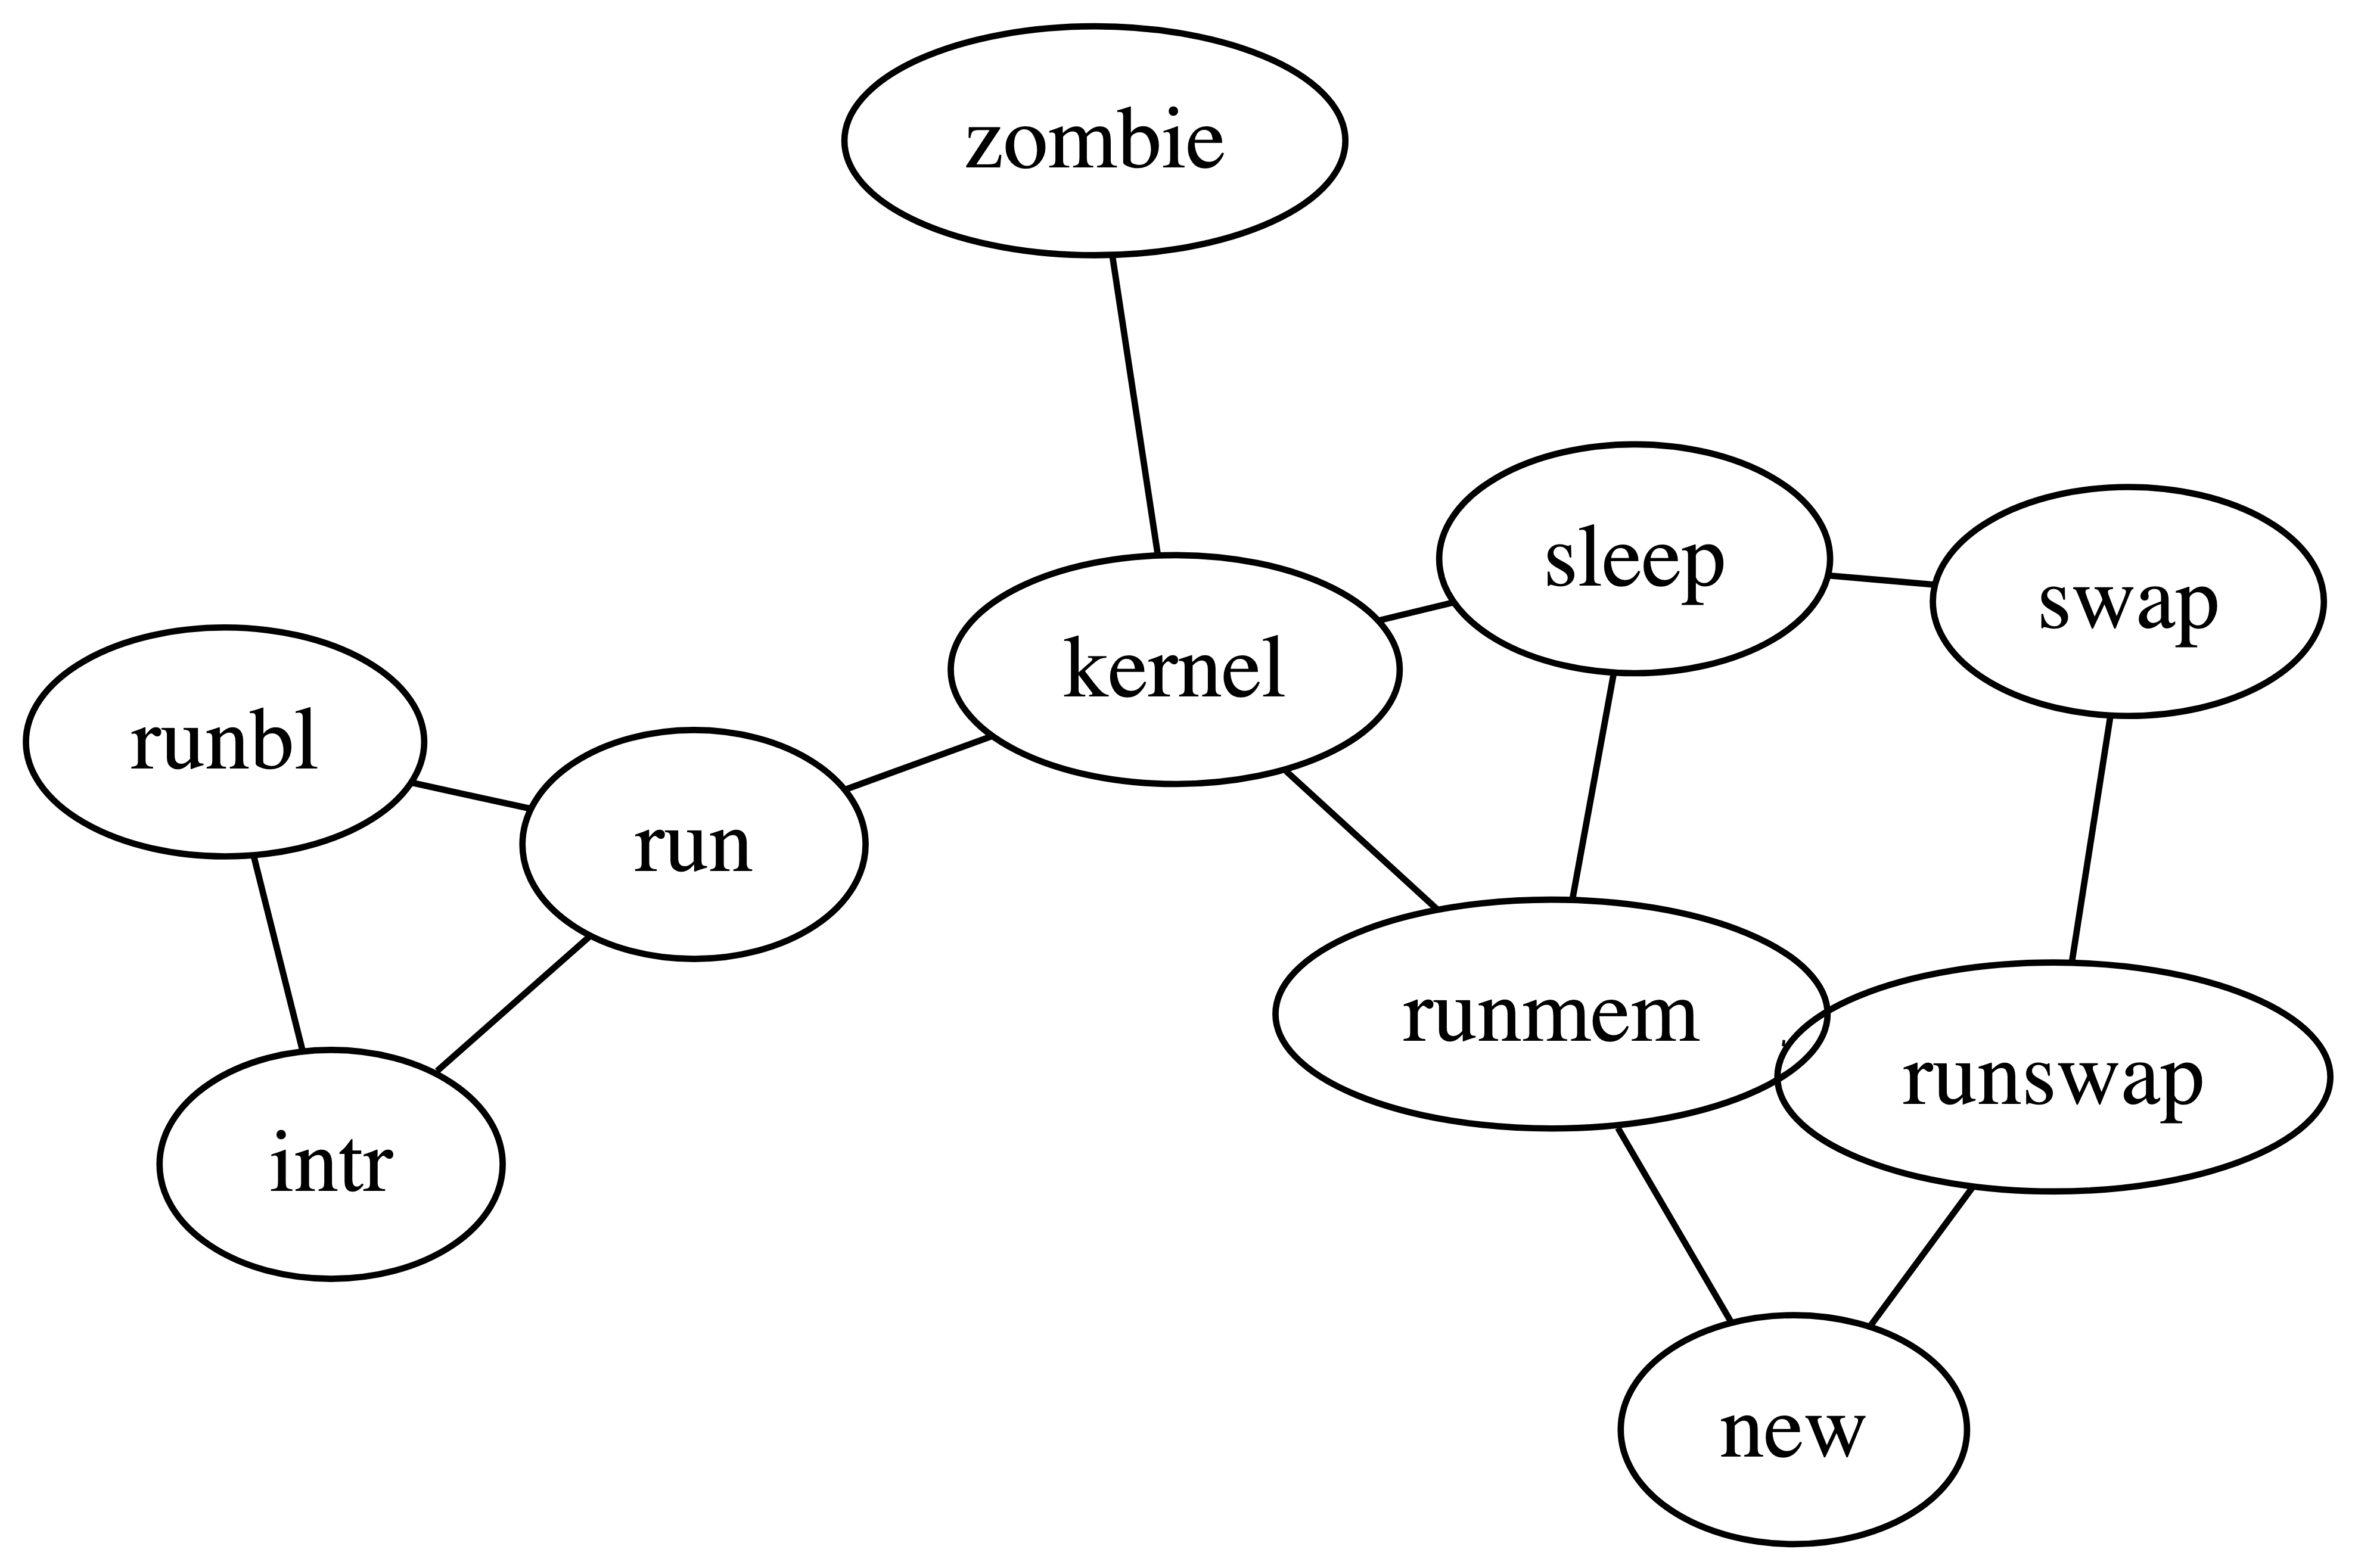
\includegraphics[width=5.5in,height=3.5in]{index_files/figure-latex/dot-figure-3.png}

}

\end{figure}

}

\caption{\label{fig-scriv14B}A graphviz graph with figure reference and
caption, using raw markup. Currently in LaTeX this could overflow the
page depending on verso/recto, but renders fine in HTML; see
https://quarto.org/docs/authoring/diagrams.html\#sizing for more
details\ldots{}}

\end{figure}

\begin{figure}

{\centering 

\begin{figure}[H]

{\centering 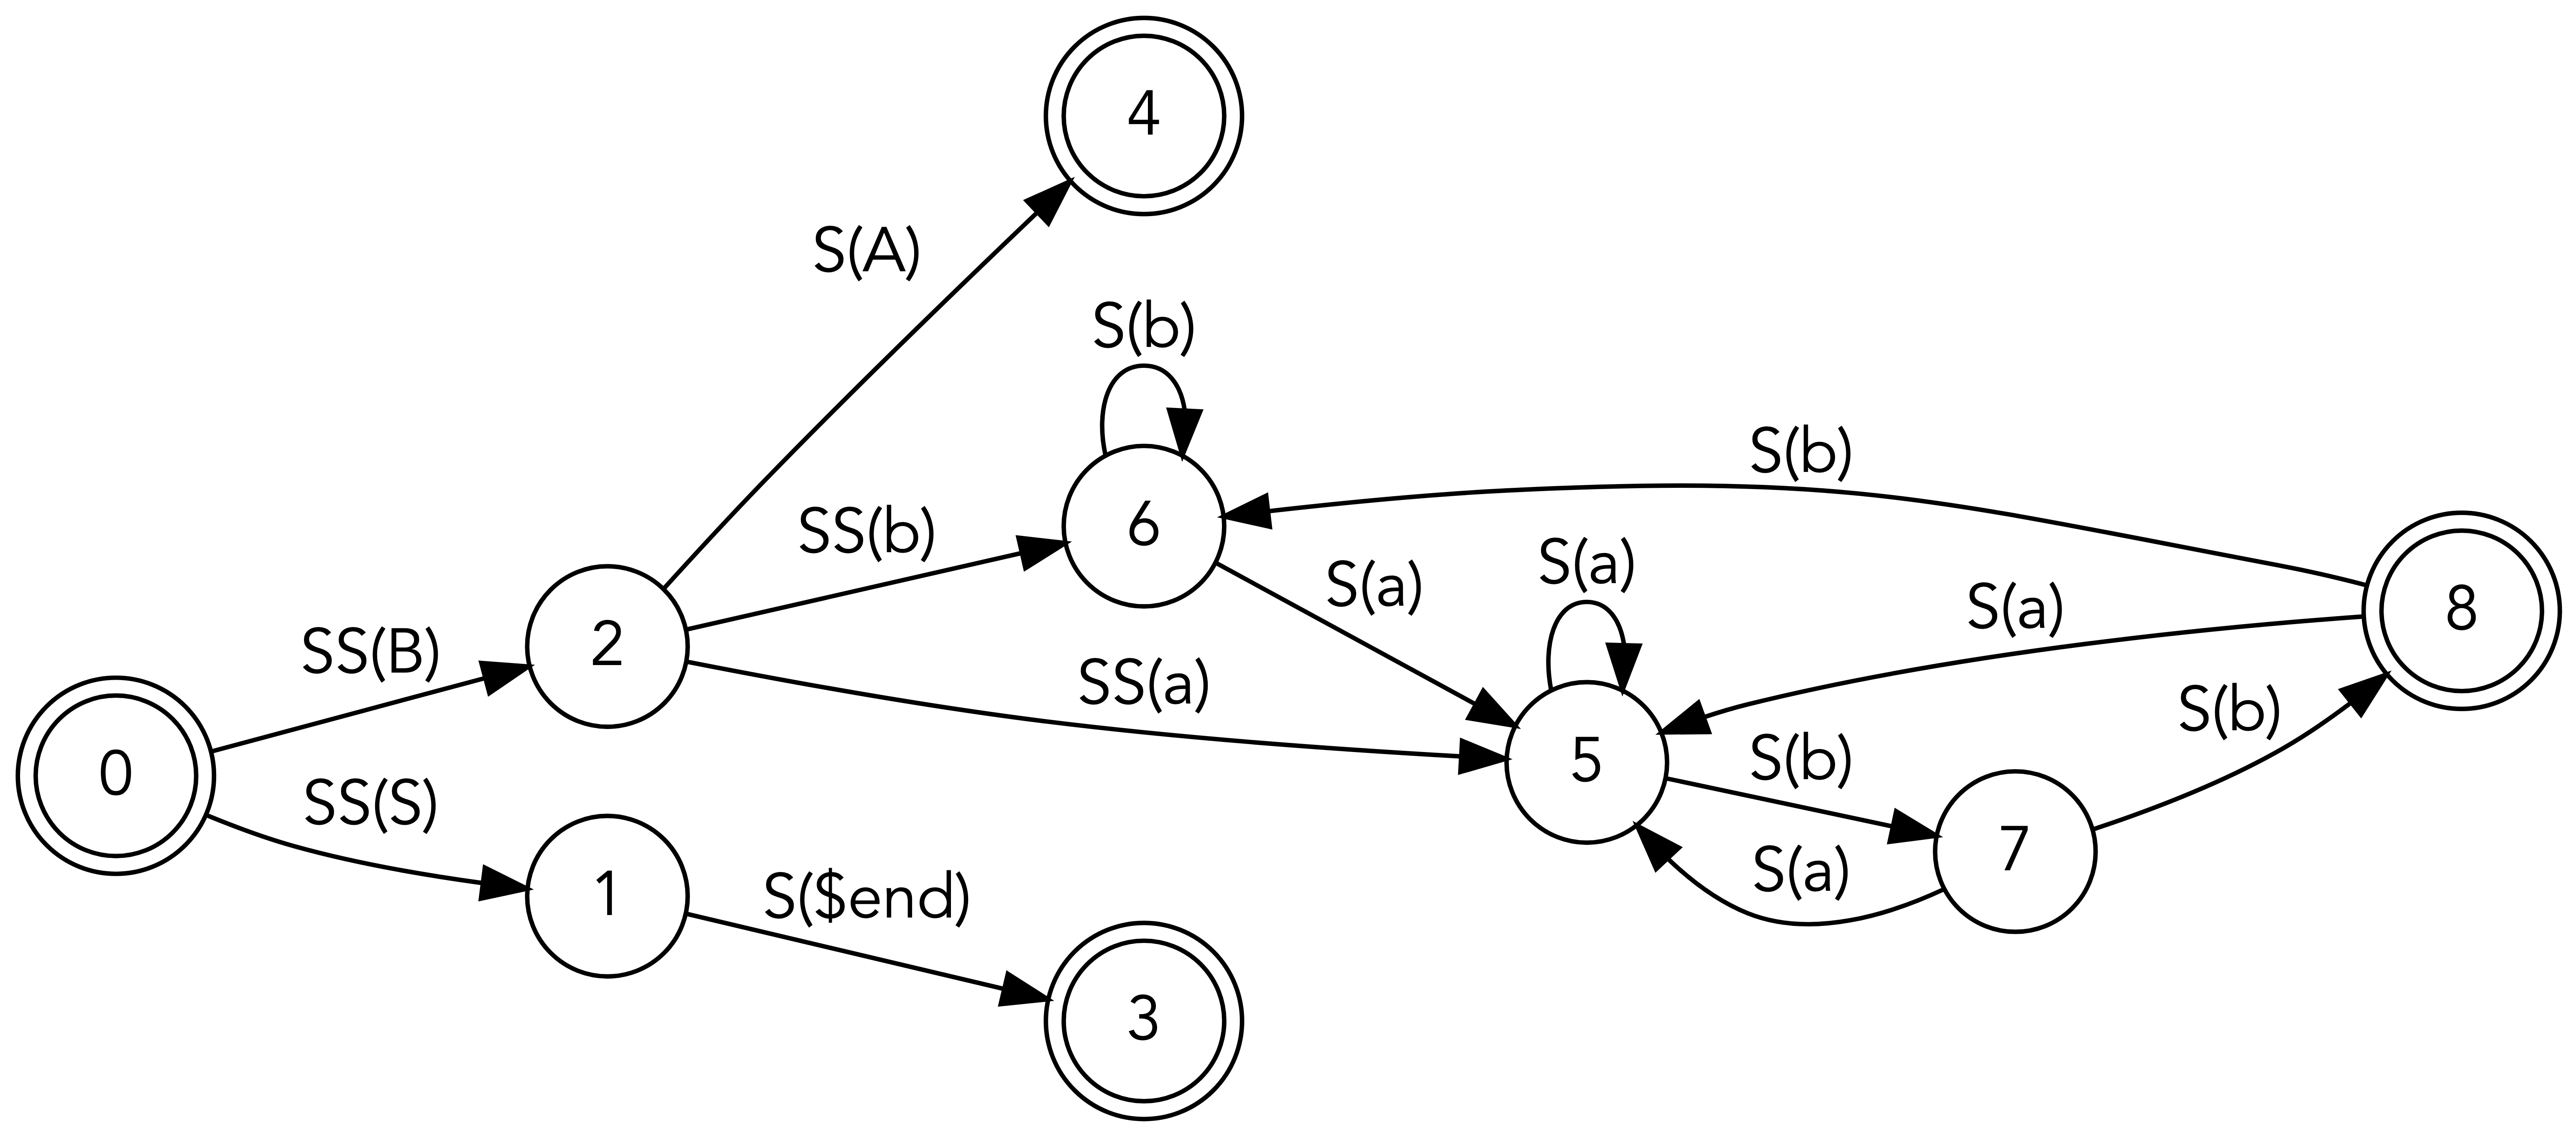
\includegraphics[width=5.5in,height=3.5in]{index_files/figure-latex/dot-figure-2.png}

}

\end{figure}

}

\caption{\label{fig-scriv15}A Graphviz-generated state machine diagram}

\end{figure}

\begin{figure}

{\centering 

\begin{figure}[H]

{\centering 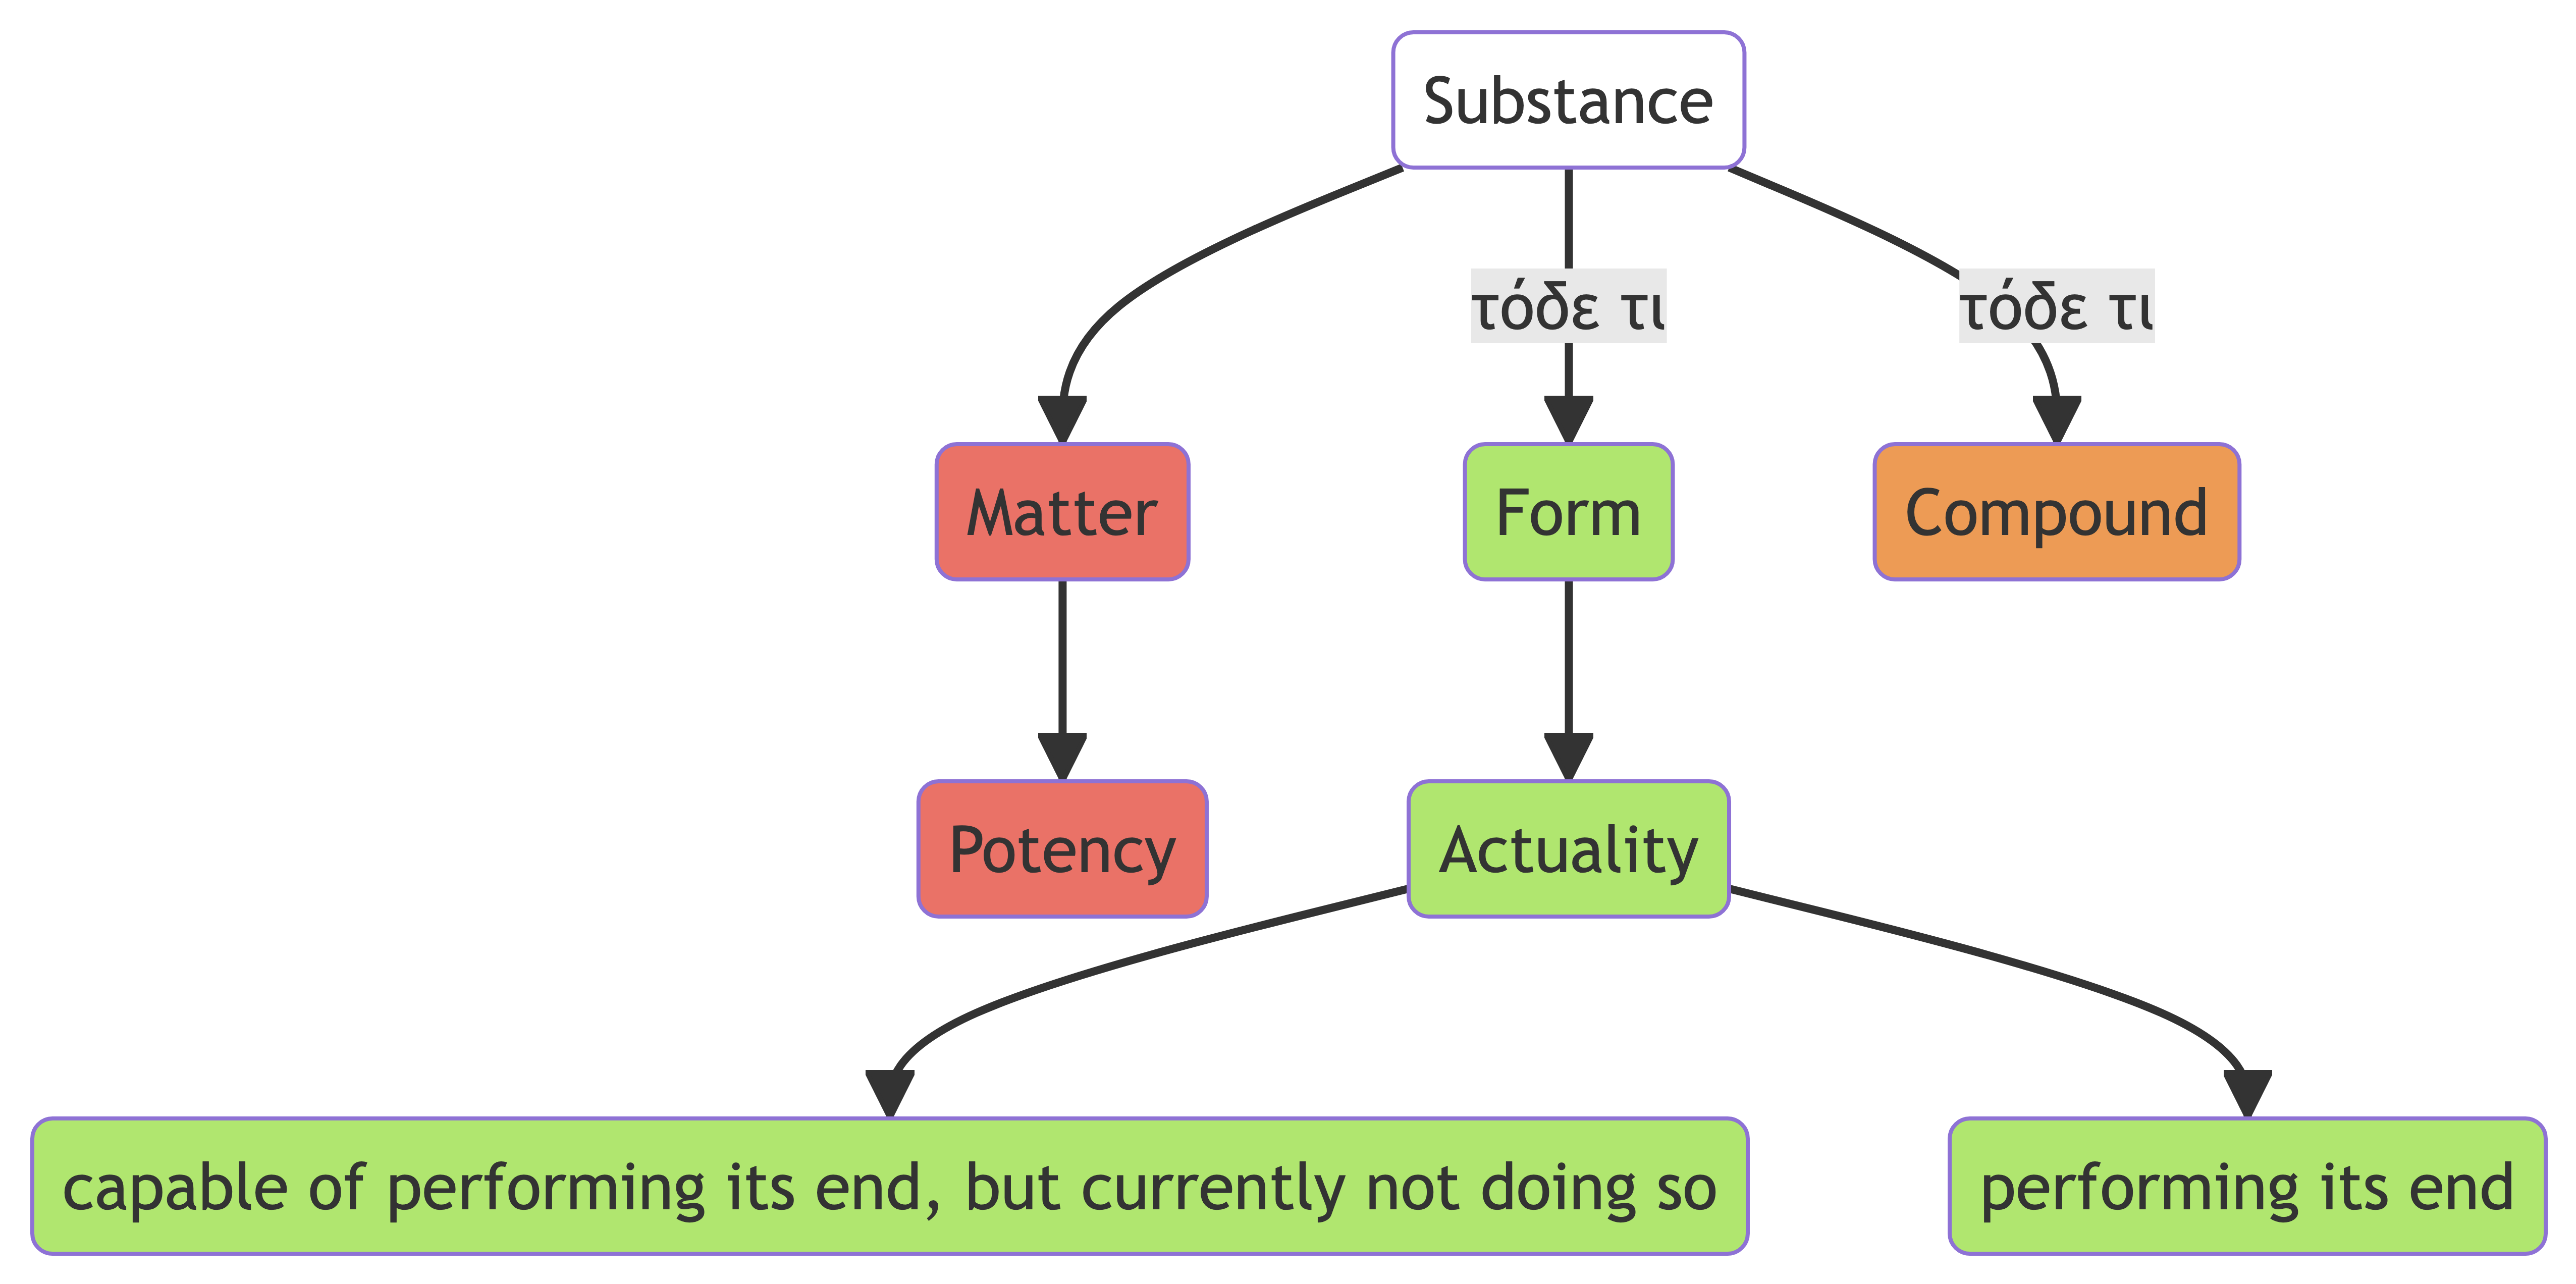
\includegraphics[width=6.65in,height=3.32in]{index_files/figure-latex/mermaid-figure-1.png}

}

\end{figure}

}

\caption{\label{fig-scriv16}Figure caption}

\end{figure}

\begin{figure}

{\centering 

\begin{figure}[H]

{\centering 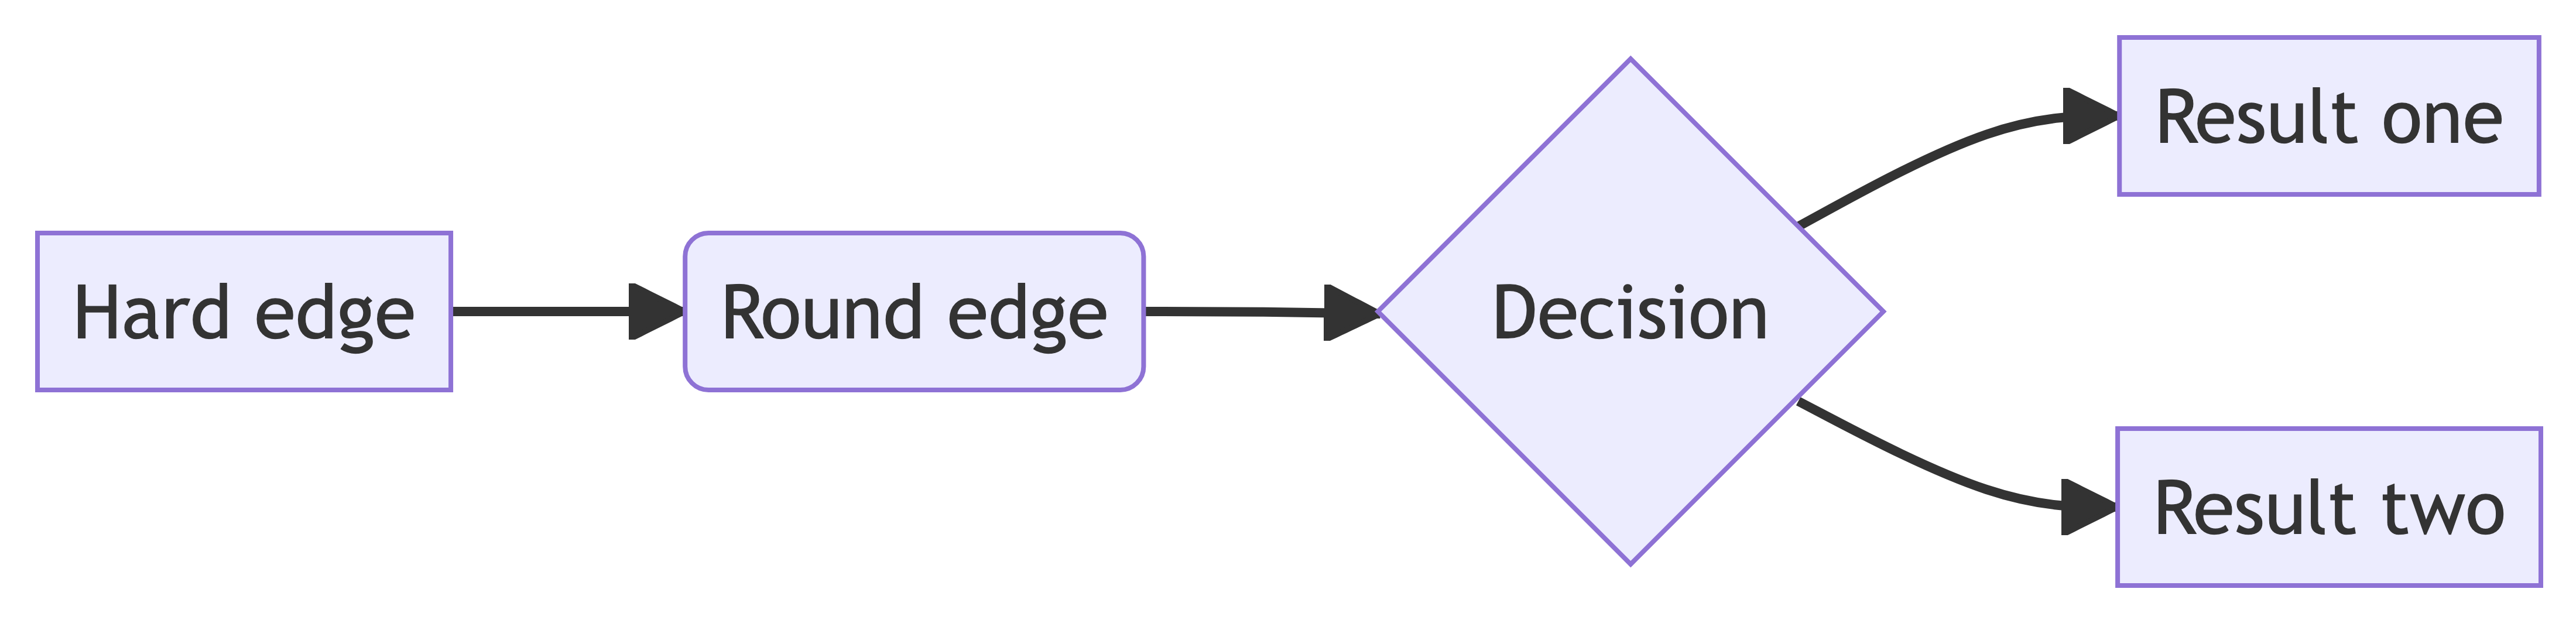
\includegraphics[width=5.73in,height=1.39in]{index_files/figure-latex/mermaid-figure-3.png}

}

\end{figure}

}

\caption{\label{fig-scriv16B}Figure caption}

\end{figure}

\hypertarget{fig-scriv17}{}
\begin{figure*}

\begin{figure}[H]

{\centering 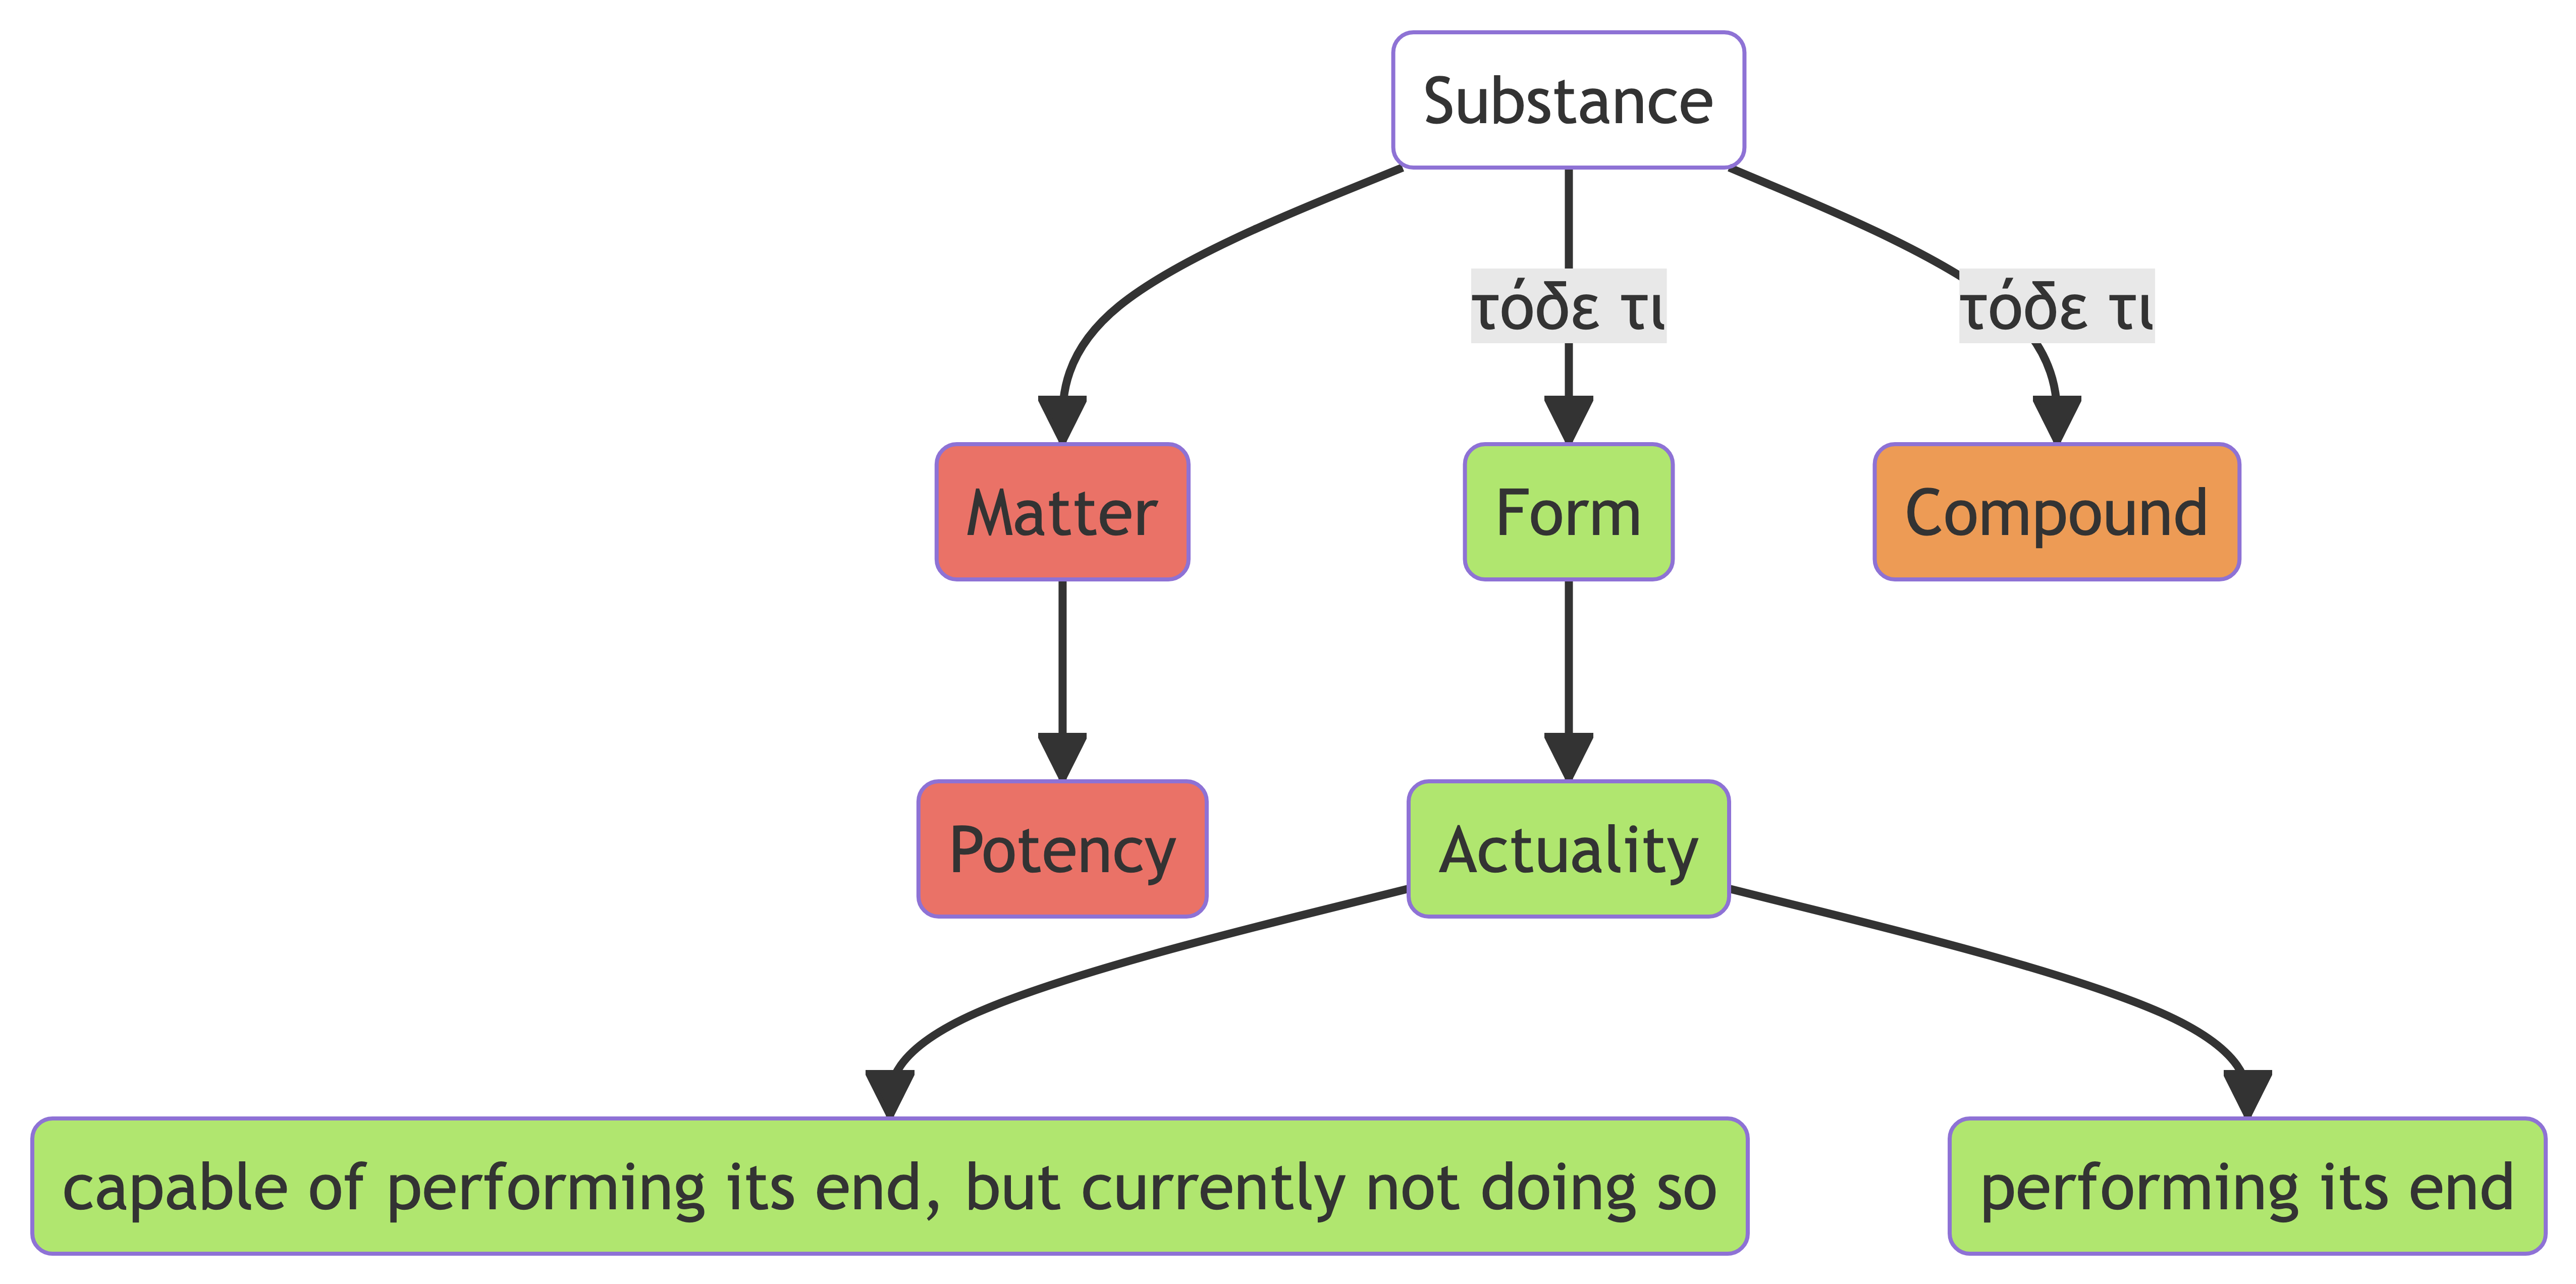
\includegraphics[width=6.65in,height=3.32in]{index_files/figure-latex/mermaid-figure-2.png}

}

\end{figure}

\label{fig-scriv17}A Mermaid figure using a Scrivener Section Type
{[}Diagram Mermaid{]}, see
https://quarto.org/docs/authoring/diagrams.html for more details

\end{figure*}

\newpage{}

\hypertarget{sec-scriv18}{%
\section{Equations}\label{sec-scriv18}}

\hypertarget{tbl-scriv18}{}
\begin{longtable}[]{@{}ccc@{}}
\toprule\noalign{}
\textbf{Element} & \textbf{Markdown Source} & \textbf{Rendered
Output} \\
\midrule\noalign{}
\endfirsthead
\toprule\noalign{}
\textbf{Element} & \textbf{Markdown Source} & \textbf{Rendered
Output} \\
\midrule\noalign{}
\endhead
\bottomrule\noalign{}
\endlastfoot
Equation & \texttt{{[}@eq-scriv19{]}} &
\protect\hypertarget{cite_73}{}{\label{cite_73}Equation~\ref{eq-scriv19}} \\
Equation & \texttt{{[}@eq-scriv20{]}} &
\protect\hypertarget{cite_74}{}{\label{cite_74}Equation~\ref{eq-scriv20}} \\
\caption{\label{tbl-scriv18}Cross-referencing equations.}\tabularnewline
\end{longtable}

\begin{equation}\protect\hypertarget{eq-scriv19}{}{t' = \frac{t - \dfrac{v}{c^{2}}x}{\sqrt{1 - \dfrac{v^{2}}{c^{2}}}}}\label{eq-scriv19}\end{equation}

\begin{equation}\protect\hypertarget{eq-scriv20}{}{t' = \frac{t - \dfrac{v}{c^{2}}x}{\sqrt{1 - \dfrac{v^{2}}{c^{2}}}}
}\label{eq-scriv20}\end{equation}

\newpage{}

\hypertarget{sec-scriv21}{%
\section{Figures}\label{sec-scriv21}}

\marginnote{\begin{footnotesize}

\enquote{I propose a toast, to my self-control. You see it helpless,
crawling on the floor.} Morphine, \emph{Cure For Pain} (1993)

\end{footnotesize}}

\hypertarget{tbl-scriv21}{}
\begin{longtable}[]{@{}ccc@{}}
\toprule\noalign{}
\textbf{Element} & \textbf{Markdown Source} & \textbf{Rendered
Output} \\
\midrule\noalign{}
\endfirsthead
\toprule\noalign{}
\textbf{Element} & \textbf{Markdown Source} & \textbf{Rendered
Output} \\
\midrule\noalign{}
\endhead
\bottomrule\noalign{}
\endlastfoot
Figure & \texttt{{[}@fig-scriv22{]}} &
\protect\hypertarget{cite_75}{}{\label{cite_75}Figure~\ref{fig-scriv22}} \\
Figure (Multipart) & \texttt{{[}@fig-scriv23{]}} &
\protect\hypertarget{cite_76}{}{\label{cite_76}Figure~\ref{fig-scriv23}} \\
Figure (Multipart) & \texttt{{[}@fig-scriv23A{]}} &
\protect\hypertarget{cite_77}{}{\label{cite_77}Figure~\ref{fig-scriv23A}} \\
Figure (Multipart) & \texttt{{[}@fig-scriv23B{]}} &
\protect\hypertarget{cite_78}{}{\label{cite_78}Figure~\ref{fig-scriv23B}} \\
Figure (Multipart) & \texttt{{[}@fig-scriv24{]}} &
\protect\hypertarget{cite_79}{}{\label{cite_79}Figure~\ref{fig-scriv24}} \\
Figure (Multipart) & \texttt{{[}@fig-scriv24A{]}} &
\protect\hypertarget{cite_80}{}{\label{cite_80}Figure~\ref{fig-scriv24A}} \\
Figure (Multipart) & \texttt{{[}@fig-scriv24B{]}} &
\protect\hypertarget{cite_81}{}{\label{cite_81}Figure~\ref{fig-scriv24B}} \\
\caption{\label{tbl-scriv21}Cross-referencing figures.}\tabularnewline
\end{longtable}

\begin{figure}

{\centering 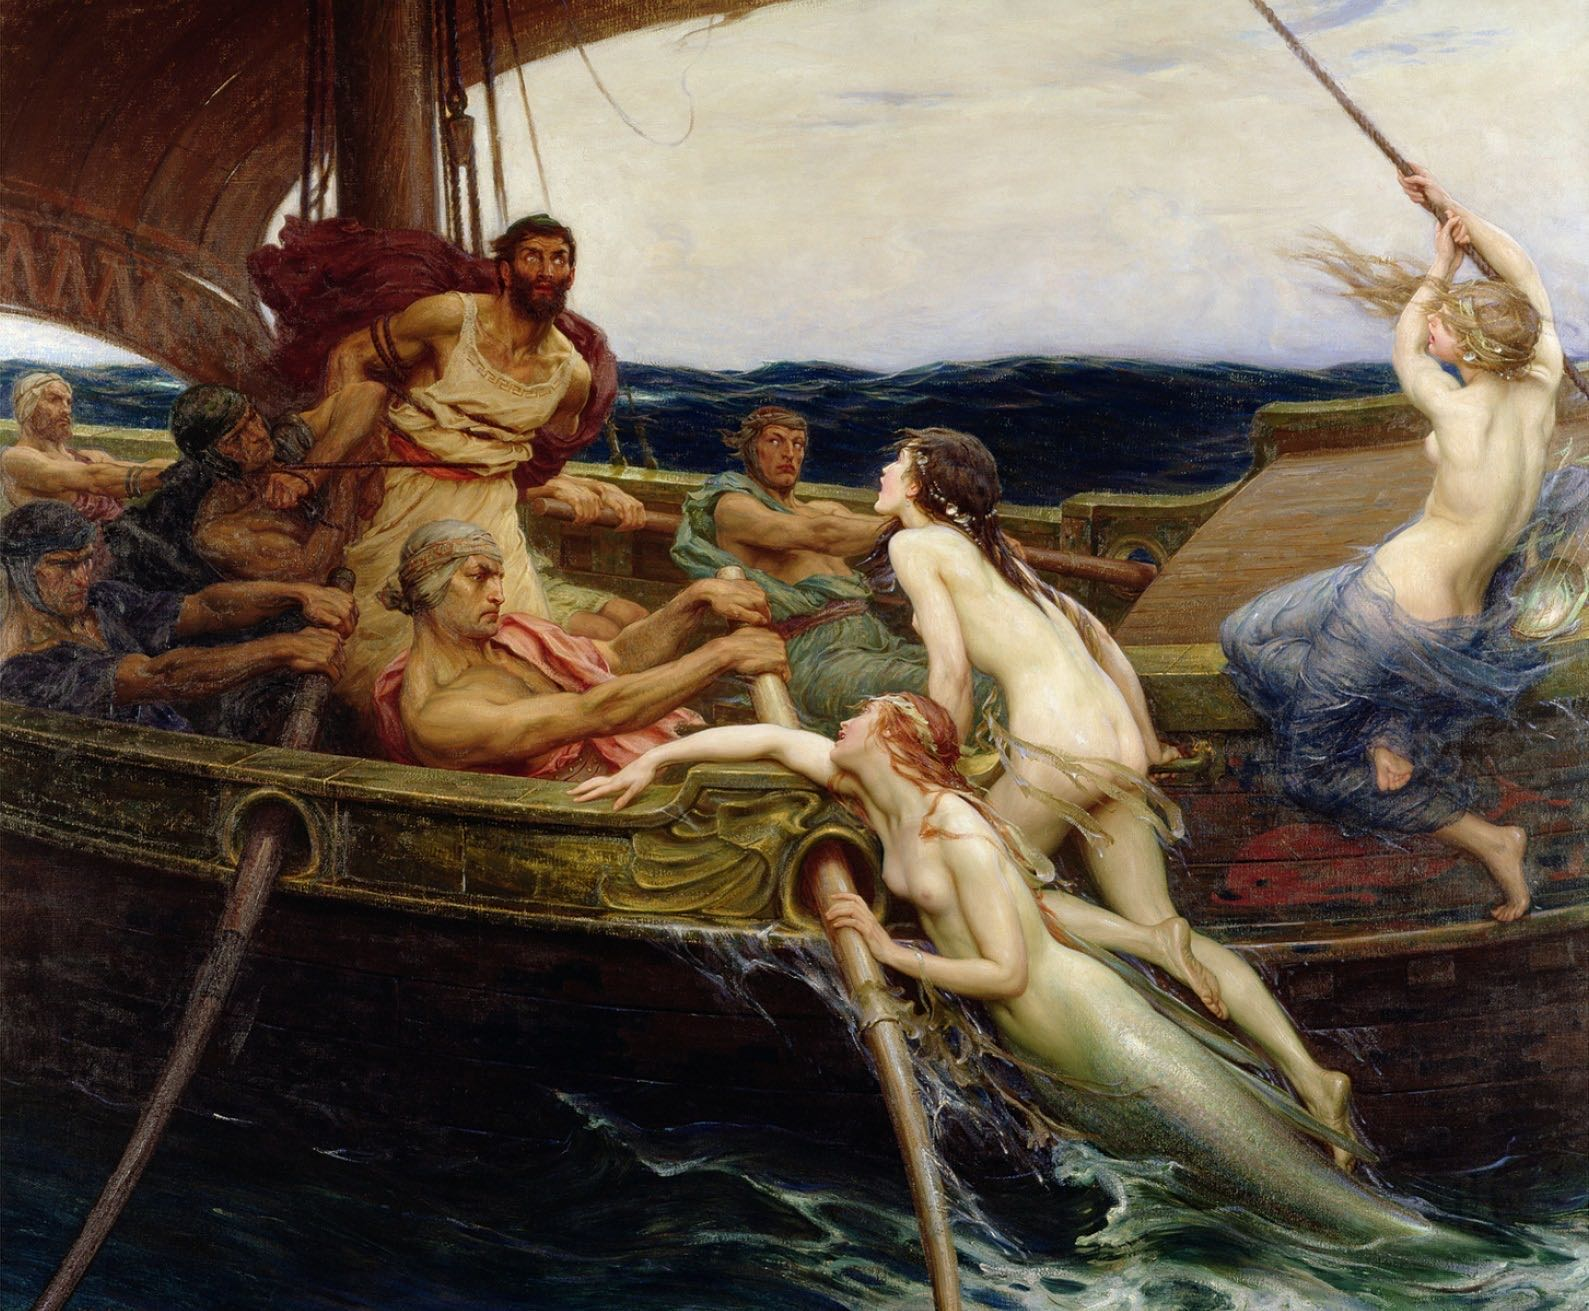
\includegraphics[width=5.0625in,height=4.1875in]{Ulysses1.jpg}

}

\caption{\label{fig-scriv22}\enquote{I propose a toast, to my
self-control. You see it crawling helpless on the floor.} - Morphine,
\emph{Cure For Pain} (1993). This figure uses custom metadata values to
identify the class, ID, width and height. The \%CA\%\hspace{0pt}
(\textbf{C}aption \textbf{A}ttributes) tag at the start of the caption
is replaced with the correct Scrivener placeholders by the compiler; see
global replacements for the details\ldots{}}

\end{figure}

\begin{figure*}

\begin{minipage}[t]{0.45\linewidth}

{\centering 

\raisebox{-\height}{

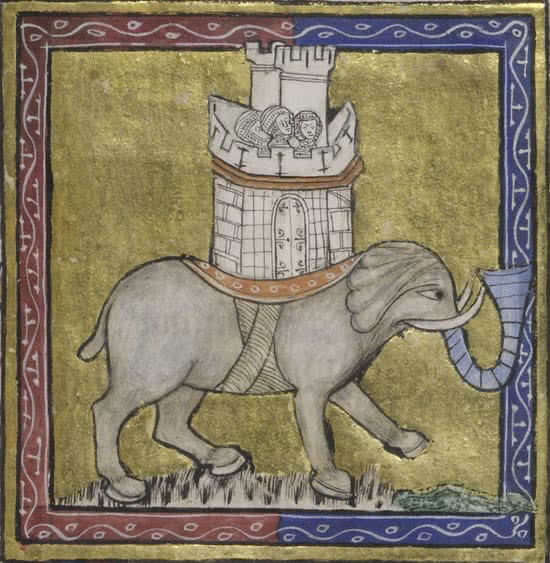
\includegraphics[width=2.55208in,height=\textheight]{Elephant2.jpg}

}

}

\subcaption{\label{fig-scriv23A}Elephant.}
\end{minipage}%
%
\begin{minipage}[t]{0.56\linewidth}

{\centering 

\raisebox{-\height}{

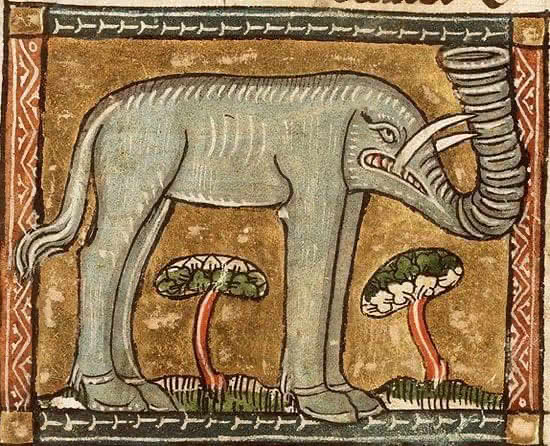
\includegraphics[width=3.1875in,height=\textheight]{Elephant3.jpg}

}

}

\subcaption{\label{fig-scriv23B}Angry elephant with a big trunk.}
\end{minipage}%

\caption{\label{fig-scriv23}This demonstrates generating a multi-panel
figure using a Scrivener Section Type {[}\ul{Multipart Figure}{]}
instead of using raw markdown as shown here. ID, Class, and Attributes
specific to the block {[}\ul{\#fig-elephants2 .column-body layout-ncol=2
layout-valign=\enquote{bottom}}{]} are saved to \ul{Custom
Metadata-\textgreater ID, Class \& Attributes}, and this is then
inserted into the markup for this chunk by the Section Layout at compile
time.}

\end{figure*}

\begin{figure*}

\begin{minipage}[t]{0.44\linewidth}

{\centering 

\raisebox{-\height}{

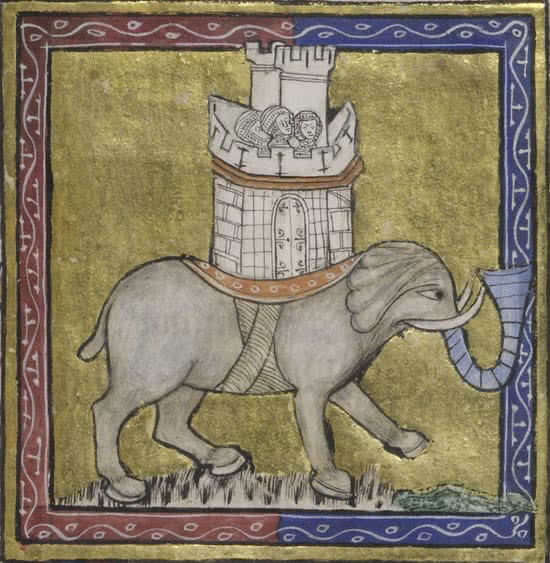
\includegraphics[width=2.53125in,height=\textheight]{Elephant2.jpg}

}

}

\subcaption{\label{fig-scriv24A}Elephant castle.}
\end{minipage}%
%
\begin{minipage}[t]{0.56\linewidth}

{\centering 

\raisebox{-\height}{

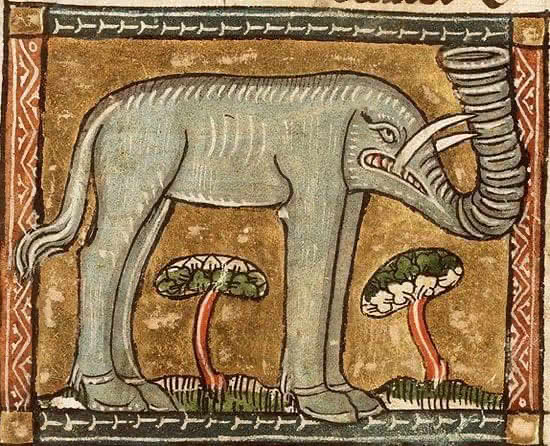
\includegraphics[width=3.16667in,height=\textheight]{Elephant3.jpg}

}

}

\subcaption{\label{fig-scriv24B}Angry elephant with a big trunk.}
\end{minipage}%

\caption{\label{fig-scriv24}Quarto allows the creation of figure panels
with sub-figures. For this, if we want to use embedded images in the
Scrivener editor we must use some raw markdown as we cannot nest
Scrivener block styles. Note we can use the Scale Image\ldots{} Tool in
Scrivener and these sizes get exported to Quarto and the output. Here we
scale both images to the same height.}

\end{figure*}

\newpage{}

\hypertarget{sec-scriv25}{%
\section{Listings}\label{sec-scriv25}}

\hypertarget{tbl-scriv25}{}
\begin{longtable}[]{@{}ccc@{}}
\toprule\noalign{}
\textbf{Element} & \textbf{Markdown Source} & \textbf{Rendered
Output} \\
\midrule\noalign{}
\endfirsthead
\toprule\noalign{}
\textbf{Element} & \textbf{Markdown Source} & \textbf{Rendered
Output} \\
\midrule\noalign{}
\endhead
\bottomrule\noalign{}
\endlastfoot
Listing & \texttt{{[}@lst-scriv26{]}} &
\protect\hypertarget{cite_82}{}{\label{cite_82}Listing~\ref{lst-scriv26}} \\
Listing & \texttt{{[}@lst-scriv27{]}} &
\protect\hypertarget{cite_83}{}{\label{cite_83}Listing~\ref{lst-scriv27}} \\
\caption{\label{tbl-scriv25}Cross-referencing listings.}\tabularnewline
\end{longtable}

\begin{codelisting}

\caption{Ruby code block. The listing Paragraph Style uses the custom
metadata of the current text document.}

\hypertarget{lst-scriv26}{%
\label{lst-scriv26}}%
\begin{Shaded}
\begin{Highlighting}[numbers=left,,]
\FunctionTok{require} \StringTok{"unicode/name"}

\NormalTok{characters }\KeywordTok{=}\OtherTok{ \%w(}\StringTok{α β γ δ ε ζ η θ ι κ λ μ ν ξ ο π ρ σ τ υ φ χ ψ ω }
\StringTok{ἀ ἄ ᾄ ἂ ᾂ ἆ ᾆ ᾀ ἁ ἅ ᾅ ἃ ᾃ ἇ ᾇ ᾁ ά ά ᾴ ὰ ᾲ ᾰ ᾶ ᾷ ᾱ ᾳ ἐ ἔ ἒ ἑ ἕ ἓ έ έ ὲ}\OtherTok{)}

\CommentTok{\# characters = \textquotesingle{}ἄ\textquotesingle{}}
\NormalTok{characters}\AttributeTok{.each} \ControlFlowTok{do} \KeywordTok{|}\NormalTok{character}\KeywordTok{|}
  \FunctionTok{puts}\NormalTok{ character}\AttributeTok{.unpack}\NormalTok{(}\VerbatimStringTok{\textquotesingle{}U*\textquotesingle{}}\NormalTok{)}\AttributeTok{.map} \KeywordTok{\{} \KeywordTok{|}\NormalTok{i}\KeywordTok{|} 
  \StringTok{"U+}\SpecialCharTok{\#\{}\NormalTok{i}\AttributeTok{.to\_s}\NormalTok{(}\DecValTok{16}\NormalTok{)}\AttributeTok{.rjust}\NormalTok{(}\DecValTok{4}\NormalTok{, }\CharTok{\textquotesingle{}0\textquotesingle{}}\NormalTok{)}\AttributeTok{.upcase}\SpecialCharTok{\}}\StringTok{"}
  \KeywordTok{\}}\AttributeTok{.join}
  \FunctionTok{puts} \DataTypeTok{Unicode}\KeywordTok{::}\DataTypeTok{Name}\AttributeTok{.of}\NormalTok{ character}
\ControlFlowTok{end}
\end{Highlighting}
\end{Shaded}

\end{codelisting}

\begin{codelisting}

\caption{The caption}

\hypertarget{lst-scriv27}{%
\label{lst-scriv27}}%
\begin{Shaded}
\begin{Highlighting}[numbers=left,,]

\ControlFlowTok{\#!/usr/bin/env ruby}
\CommentTok{\# frozen\_string\_literal: false}

\DataTypeTok{Encoding}\AttributeTok{.default\_external} \KeywordTok{=} \DataTypeTok{Encoding}\KeywordTok{::}\DataTypeTok{UTF\_8}

\DataTypeTok{Dir}\KeywordTok{[}\StringTok{"}\SpecialCharTok{\#\{}\NormalTok{\_\_dir\_\_}\SpecialCharTok{\}}\StringTok{/Ruby/**/*.rb"}\KeywordTok{]}\AttributeTok{.each} \ControlFlowTok{do} \KeywordTok{|}\NormalTok{file}\KeywordTok{|}
  \FunctionTok{require\_relative}\NormalTok{ file}
\ControlFlowTok{end}
\end{Highlighting}
\end{Shaded}

\end{codelisting}

\begin{codelisting}

\caption{My Ruby code block.}

\hypertarget{lst-scriv28}{%
\label{lst-scriv28}}%
\begin{Shaded}
\begin{Highlighting}[numbers=left,,]
\FunctionTok{require} \StringTok{"unicode/name"}

\NormalTok{characters }\KeywordTok{=}\OtherTok{ \%w(}\StringTok{α β γ δ ε ζ η θ ι κ λ μ ν ξ ο π ρ σ τ υ φ χ ψ ω}\OtherTok{)}

\CommentTok{\# characters = \textquotesingle{}ἄ\textquotesingle{}}
\NormalTok{characters}\AttributeTok{.each} \ControlFlowTok{do} \KeywordTok{|}\NormalTok{character}\KeywordTok{|}
  \FunctionTok{puts}\NormalTok{ character}\AttributeTok{.unpack}\NormalTok{(}\VerbatimStringTok{\textquotesingle{}U*\textquotesingle{}}\NormalTok{)}\AttributeTok{.map} \KeywordTok{\{} \KeywordTok{|}\NormalTok{i}\KeywordTok{|} 
    \StringTok{"U+}\SpecialCharTok{\#\{}\NormalTok{i}\AttributeTok{.to\_s}\NormalTok{(}\DecValTok{16}\NormalTok{)}\AttributeTok{.rjust}\NormalTok{(}\DecValTok{4}\NormalTok{, }\CharTok{\textquotesingle{}0\textquotesingle{}}\NormalTok{)}\AttributeTok{.upcase}\SpecialCharTok{\}}\StringTok{"}
  \KeywordTok{\}}\AttributeTok{.join}
  \FunctionTok{puts} \DataTypeTok{Unicode}\KeywordTok{::}\DataTypeTok{Name}\AttributeTok{.of}\NormalTok{ character}
\ControlFlowTok{end}
\end{Highlighting}
\end{Shaded}

\end{codelisting}

\newpage{}

\hypertarget{sec-scriv29}{%
\section{Tables}\label{sec-scriv29}}

\hypertarget{tbl-scriv29}{}
\begin{longtable}[]{@{}ccc@{}}
\toprule\noalign{}
\textbf{Element} & \textbf{Markdown Source} & \textbf{Rendered
Output} \\
\midrule\noalign{}
\endfirsthead
\toprule\noalign{}
\textbf{Element} & \textbf{Markdown Source} & \textbf{Rendered
Output} \\
\midrule\noalign{}
\endhead
\bottomrule\noalign{}
\endlastfoot
Table & \texttt{{[}@tbl-scriv30{]}} &
\protect\hypertarget{cite_84}{}{\label{cite_84}Table~\ref{tbl-scriv30}} \\
Table & \texttt{{[}@tbl-scriv31{]}} &
\protect\hypertarget{cite_85}{}{\label{cite_85}Table~\ref{tbl-scriv31}} \\
Table (Multipart) & \texttt{{[}@tbl-scriv32{]}} &
\protect\hypertarget{cite_86}{}{\label{cite_86}Table~\ref{tbl-scriv32}} \\
Table (Multipart) & \texttt{{[}@tbl-scriv32A{]}} &
\protect\hypertarget{cite_87}{}{\label{cite_87}Table~\ref{tbl-scriv32A}} \\
Table (Multipart) & \texttt{{[}@tbl-scriv32B{]}} &
\protect\hypertarget{cite_88}{}{\label{cite_88}Table~\ref{tbl-scriv32B}} \\
\caption{\label{tbl-scriv29}Cross-referencing tables.}\tabularnewline
\end{longtable}

\hypertarget{tbl-scriv30}{}
\begin{longtable}[]{@{}lll@{}}
\toprule\noalign{}
1 & 2 & 3 \\
\midrule\noalign{}
\endfirsthead
\toprule\noalign{}
1 & 2 & 3 \\
\midrule\noalign{}
\endhead
\bottomrule\noalign{}
\endlastfoot
4 & 5 & 6 \\
\caption{\label{tbl-scriv30}This table uses \ul{Text} as the
\textbf{Section Type}, and \ul{Table Caption} as the \textbf{Paragraph
Style} for the caption.}\tabularnewline
\end{longtable}

\hypertarget{tbl-scriv31}{}
\begin{longtable}[]{@{}lll@{}}
\toprule\noalign{}
1 & 2 & 3 \\
\midrule\noalign{}
\endfirsthead
\toprule\noalign{}
1 & 2 & 3 \\
\midrule\noalign{}
\endhead
\bottomrule\noalign{}
\endlastfoot
4 & 5 & 6 \\
\caption{\label{tbl-scriv31}This is an example of \texttt{Table} as
\textbf{Section Type}. The caption and the remaining attributes are
added as part of the Section Type markup.}\tabularnewline
\end{longtable}

\begin{table}

\begin{minipage}[t]{\linewidth}

{\centering 

\begin{tabular}[t]{cccc}
\toprule
\textbf{Element} & \textbf{Prefix} & \textbf{Markdown
Source} & \textbf{Rendered Output}\\
\midrule
Equation A & eq & A & B\\
Equation A & eq & C & D\\
Listing A & lst & E & F\\
\bottomrule
\end{tabular}

}

\subcaption{\label{tbl-scriv32A}First Table}
\end{minipage}%
\newline
\begin{minipage}[t]{\linewidth}

{\centering 

\begin{tabular}[t]{cccc}
\toprule
\textbf{Element} & \textbf{Prefix} & \textbf{Markdown
Source} & \textbf{Rendered Output}\\
\midrule
Equation B & eq & A & B\\
Equation B & eq & C & D\\
Listing B & lst & E & F\\
\bottomrule
\end{tabular}

}

\subcaption{\label{tbl-scriv32B}Second Table}
\end{minipage}%

\caption{\label{tbl-scriv32}This is a markdown multi-table panel with
two sub-tables generated using a Section Type {[}\ul{Multipart
Table}{]}. Note that Custom Metadata holds the cross-referencing label,
layout class, and the attributes for this multipart table, which will be
added by the Section Layout by the compiler, using the Scrivener
placeholders:
\ul{\textless\hspace{0pt}\$\hspace{0pt}\hspace{0pt}custom:Class\textgreater{}}
\ul{\textless\hspace{0pt}\$\hspace{0pt}\hspace{0pt}custom:Attributes\textgreater{}}.}

\end{table}

\newpage{}

\hypertarget{sec-scriv33}{%
\section{Sections}\label{sec-scriv33}}

The text sections can be referenced with \textbf{Character Styles}, and
created with \textbf{Paragraph Styles} or \textbf{Section Types}. As
before, all of these receive automatic IDs.

\hypertarget{tbl-scriv33}{}
\begin{longtable}[]{@{}ccc@{}}
\toprule\noalign{}
\textbf{Element} & \textbf{Markdown Source} & \textbf{Rendered
Output} \\
\midrule\noalign{}
\endfirsthead
\toprule\noalign{}
\textbf{Element} & \textbf{Markdown Source} & \textbf{Rendered
Output} \\
\midrule\noalign{}
\endhead
\bottomrule\noalign{}
\endlastfoot
Section & \texttt{{[}@sec-scriv33{]}} &
\protect\hypertarget{cite_89}{}{\label{cite_89}Section~\ref{sec-scriv33}} \\
Section & \texttt{{[}@sec-scriv34{]}} &
\protect\hypertarget{cite_90}{}{\label{cite_90}Section~\ref{sec-scriv34}} \\
Section & \texttt{{[}@sec-scriv36{]}} &
\protect\hypertarget{cite_91}{}{\label{cite_91}Section~\ref{sec-scriv36}} \\
Section & \texttt{{[}@sec-scriv37{]}} &
\protect\hypertarget{cite_92}{}{\label{cite_92}Section~\ref{sec-scriv37}} \\
Section & \texttt{{[}@sec-scriv38{]}} &
\protect\hypertarget{cite_93}{}{\label{cite_93}Section~\ref{sec-scriv38}} \\
\caption{\label{tbl-scriv33}Cross-referencing sections.}\tabularnewline
\end{longtable}

Note that the unnumbered section cannot be referenced.

\hypertarget{sec-scriv34}{%
\subsection{Section}\label{sec-scriv34}}

This is an example of the \ul{Section} section type.

\hypertarget{sec-scriv35}{%
\subsection*{Section \{-\}}\label{sec-scriv35}}
\addcontentsline{toc}{subsection}{Section \{-\}}

\protect\hypertarget{scriv35}{}{}

This is an example of the \ul{Section \{-\}} section type.

\hypertarget{sec-scriv36}{%
\subsection{Heading}\label{sec-scriv36}}

\hypertarget{sec-scriv37}{%
\subsection{Heading + Break}\label{sec-scriv37}}

This is an example of the \ul{Heading + Break} section type.

\newpage{}

\newpage{}

\hypertarget{sec-scriv38}{%
\subsection{Section + Break}\label{sec-scriv38}}

This is an example of the \ul{Section + Break} section type.

\newpage{}

\hypertarget{sec-scriv39}{%
\section{Footnotes}\label{sec-scriv39}}

We can use also use a \textbf{Section Type} to create and a
\textbf{Character Style} (\ul{Footnote}) to reference footnotes using
the standard identifier.\footnote{\protect\hypertarget{scriv40}{}{} This
  strategy has the outstanding advantage of allowing us to use, that is
  right, you guessed it, \textbf{Paragraph Styles} and \textbf{Character
  Styles} in footnotes.}

There is one small caveat: the user has to remember to \ul{always add
two empty spaces} before each new \textbf{paragraph} in the footnote
environment. One option we have not to worry about this is using the
\ul{Footnote Text} \textbf{Paragraph Style}.

\hypertarget{sec-scriv41}{%
\chapter{Citations}\label{sec-scriv41}}

Part of the motivation behind ScrivQ comes from another project I
co-developed: the
\href{https://bcdavasconcelos.github.io/citetools}{Cite Tools} extension
for \href{https://pandoc.org}{Pandoc} and
\href{https://quarto.org}{Quarto}.

As I was first starting to use
\href{https://en.wikipedia.org/wiki/CiteProc}{Citeproc}, coming from the
jurassic
\textbf{\href{https://en.wikipedia.org/wiki/BibTeX\#Entry_types}{BibTeX}},
I was exceptionally pleased with its speed and reliability. Apart from
being \emph{a lot} faster, it would produce the same output across all
supported formats (which amounts to over 60). Out-of-the-box, however,
it lacked support for really ordinary \textbf{BibTeX functionalities},
such as the ability to split the bibliography into multiple sections, or
the ability to cite arbitrary fields of the references (\emph{e.g.}
using \texttt{citetitle}, \texttt{citeauthor}, \texttt{citefield}). It
also lacked the interesting \textbf{backref} option afforded by
\textbf{BibTeX} used in conjunction with \textbf{HyperRef} to create
linked indexes of citations.

\begin{figure}

{\centering 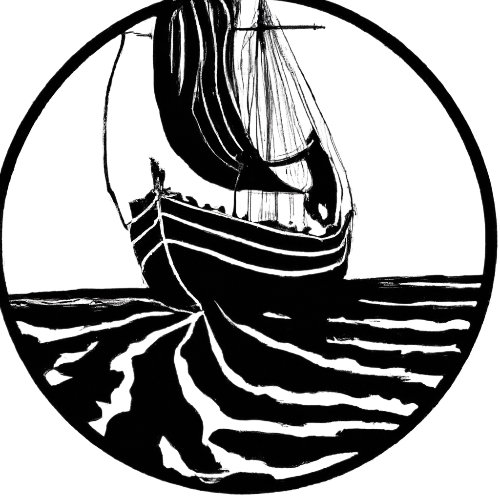
\includegraphics[width=2.875in,height=2.875in]{citetools.png}

}

\caption{\label{fig-scriv41}Cite Tool bundles together several lua
filters to address complex bibliography demands while keeping the output
consistent across formats. If you have suggestions for improvements or
bug reports, please
\href{https://github.com/bcdavasconcelos/citetools/issues/new/choose}{open
an issue at the citetools repository}. Logo image generated with Dall-E
using \enquote{\emph{Enso-like round black and white painting with
ancient greek war-ship with a man tied to the mast as prompt}}.}

\end{figure}

To step around these limitations, I started tinkering with existing
filters available on GitHub (all of them by Albert Krewinkel), and
co-developed Cite Field, to create \textbf{Cite Tools}, an extension for
Quarto and Pandoc that allows the easy creation of a \textbf{Multipart
Bibliography} (\emph{e.g.} split in \emph{primary} and \emph{secondary}
sources, see
\protect\hypertarget{cite_94}{}{\label{cite_94}Figure~\ref{fig-scriv165A}}),
the citation of arbitrary fields of the references (see
\protect\hypertarget{cite_95}{}{\label{cite_95}Figure~\ref{fig-scriv165B}})\footnote{In
  the official nomenclature, CSL has variables, BibTeX has fields, and
  RIS has tags. As a general rule, we have stuck to the term fields.},
and the linking of each bibliography entry back to its in-text
occurrences (see
\protect\hypertarget{cite_96}{}{\label{cite_96}Figure~\ref{fig-scriv165C}})\footnote{Linked
  glossaries can also easily be created by dressing them as
  bibliography.}. The filters are built-in, and the front matter is set
up so that the necessary files are automatically created during
compilation.

\begin{tcolorbox}[enhanced jigsaw, rightrule=.15mm, opacityback=0, arc=.35mm, colback=white, toprule=.15mm, breakable, bottomrule=.15mm, left=2mm, colframe=quarto-callout-warning-color-frame, leftrule=.75mm]
\begin{minipage}[t]{5.5mm}
\textcolor{quarto-callout-warning-color}{\faExclamationTriangle}
\end{minipage}%
\begin{minipage}[t]{\textwidth - 5.5mm}

\textbf{Deleting Cite Tools from ScrivQ \ul{will cause the compilation
to fail}.}\vspace{2mm}

\end{minipage}%
\end{tcolorbox}

\begin{tcolorbox}[enhanced jigsaw, rightrule=.15mm, opacityback=0, arc=.35mm, colback=white, toprule=.15mm, breakable, bottomrule=.15mm, left=2mm, colframe=quarto-callout-tip-color-frame, leftrule=.75mm]
\begin{minipage}[t]{5.5mm}
\textcolor{quarto-callout-tip-color}{\faLightbulb}
\end{minipage}%
\begin{minipage}[t]{\textwidth - 5.5mm}

If you need to use \textbf{Cite Tools }in an ordinary Quarto project,
use \texttt{quarto\ install\ extension\ bcdavasconcelos/citetools} to
install it.

\end{minipage}%
\end{tcolorbox}

\hypertarget{sec-scriv42}{%
\section{Multipart Bibliography}\label{sec-scriv42}}

In many areas of research, the ability to split the bibliography into
sections is a condition \emph{sine qua non} for publishing. In the
humanities, for example, there are usually \emph{primary} and
\emph{secondary} sources. In philosophy, even, they can be very nuanced
with sections dedicated to original sources, translations, commentaries,
and so on. The \textbf{Section Type} titled
\texttt{Multipart\ Bibliography} can be used to create as many new
bibliography sections as necessary. Add the references that should print
there to the text, and let it know in the custom metadata
\texttt{\textless{}\textbackslash{}\$custom:Attributes\textgreater{}}
the format being used (\emph{e.g.} \texttt{bib}, \texttt{yml},
\texttt{ris}; \textbf{no dot, just the extension}).

\begin{tcolorbox}[enhanced jigsaw, rightrule=.15mm, bottomtitle=1mm, colback=white, toptitle=1mm, left=2mm, colbacktitle=quarto-callout-tip-color!10!white, opacitybacktitle=0.6, opacityback=0, arc=.35mm, leftrule=.75mm, toprule=.15mm, titlerule=0mm, breakable, coltitle=black, bottomrule=.15mm, colframe=quarto-callout-tip-color-frame, title=\textcolor{quarto-callout-tip-color}{\faLightbulb}\hspace{0.5em}{Bibliography formats}]

Speaking about formats, the most common bibliography formats are
\href{https://docs.citationstyles.org/en/stable/specification.html}{CSL-YAML},
\href{https://docs.citationstyles.org/en/stable/specification.html}{CSL-JSON},
\href{https://en.wikipedia.org/wiki/BibTeX\#Entry_types}{BibTeX}, and
\href{https://en.wikipedia.org/wiki/RIS_(file_format)\#Type_of_reference}{RIS}.
Internally, \textbf{Pandoc} and \textbf{Quarto} use the CSL
(\textbf{C}itation \textbf{S}tyle \textbf{L}anguage) to handle
bibliography, so \textbf{CSL-YAML} and \textbf{CSL-JSON} perform much
better (up to 10 times faster) than older formats like \textbf{BibTeX}
or \textbf{RIS} that will have to be converted by \textbf{Pandoc} before
it can be understood.

\end{tcolorbox}

ScrivQ provides all the data needed for the project to be compiled.
Before you can use Citeproc on your projects, you will need to generate
your bibliography data. In principle, nothing stops you from manually,
or semi-manually, keeping a bibliography in Scrivener, but this is not
very easy to manage if you have many projects sharing the same
references. (Luckily, in this regard, Scrivener offers the best text
comparison tools I can think of). The best alternative, it seems, is to
rely on specialized software such as Zotero, Bookends, Bibdesk (also
JabRef, Endnote, and
\href{en.wikipedia.org/wiki/Comparison_of_reference_management_software}{others})\footnote{If
  you are using macOS, check Bookends and Bibdesk; and, on all
  platforms, definitively get Zotero as well.}. These programs allow you
to edit your bibliography and easily export it in the desired format,
which can be copied and pasted to different Scrivener projects. Zotero
even offers an API that can be used to download shared libraries by
merely accessing a link, such as
\texttt{https://api.zotero.org/groups/}\ul{LibraryID}\texttt{/items?format=bibtex\&limit=999}
where \texttt{LibraryID} corresponds to the library's 7-digit code
(visible in the middle of the library URL).

\begin{figure}

{\centering 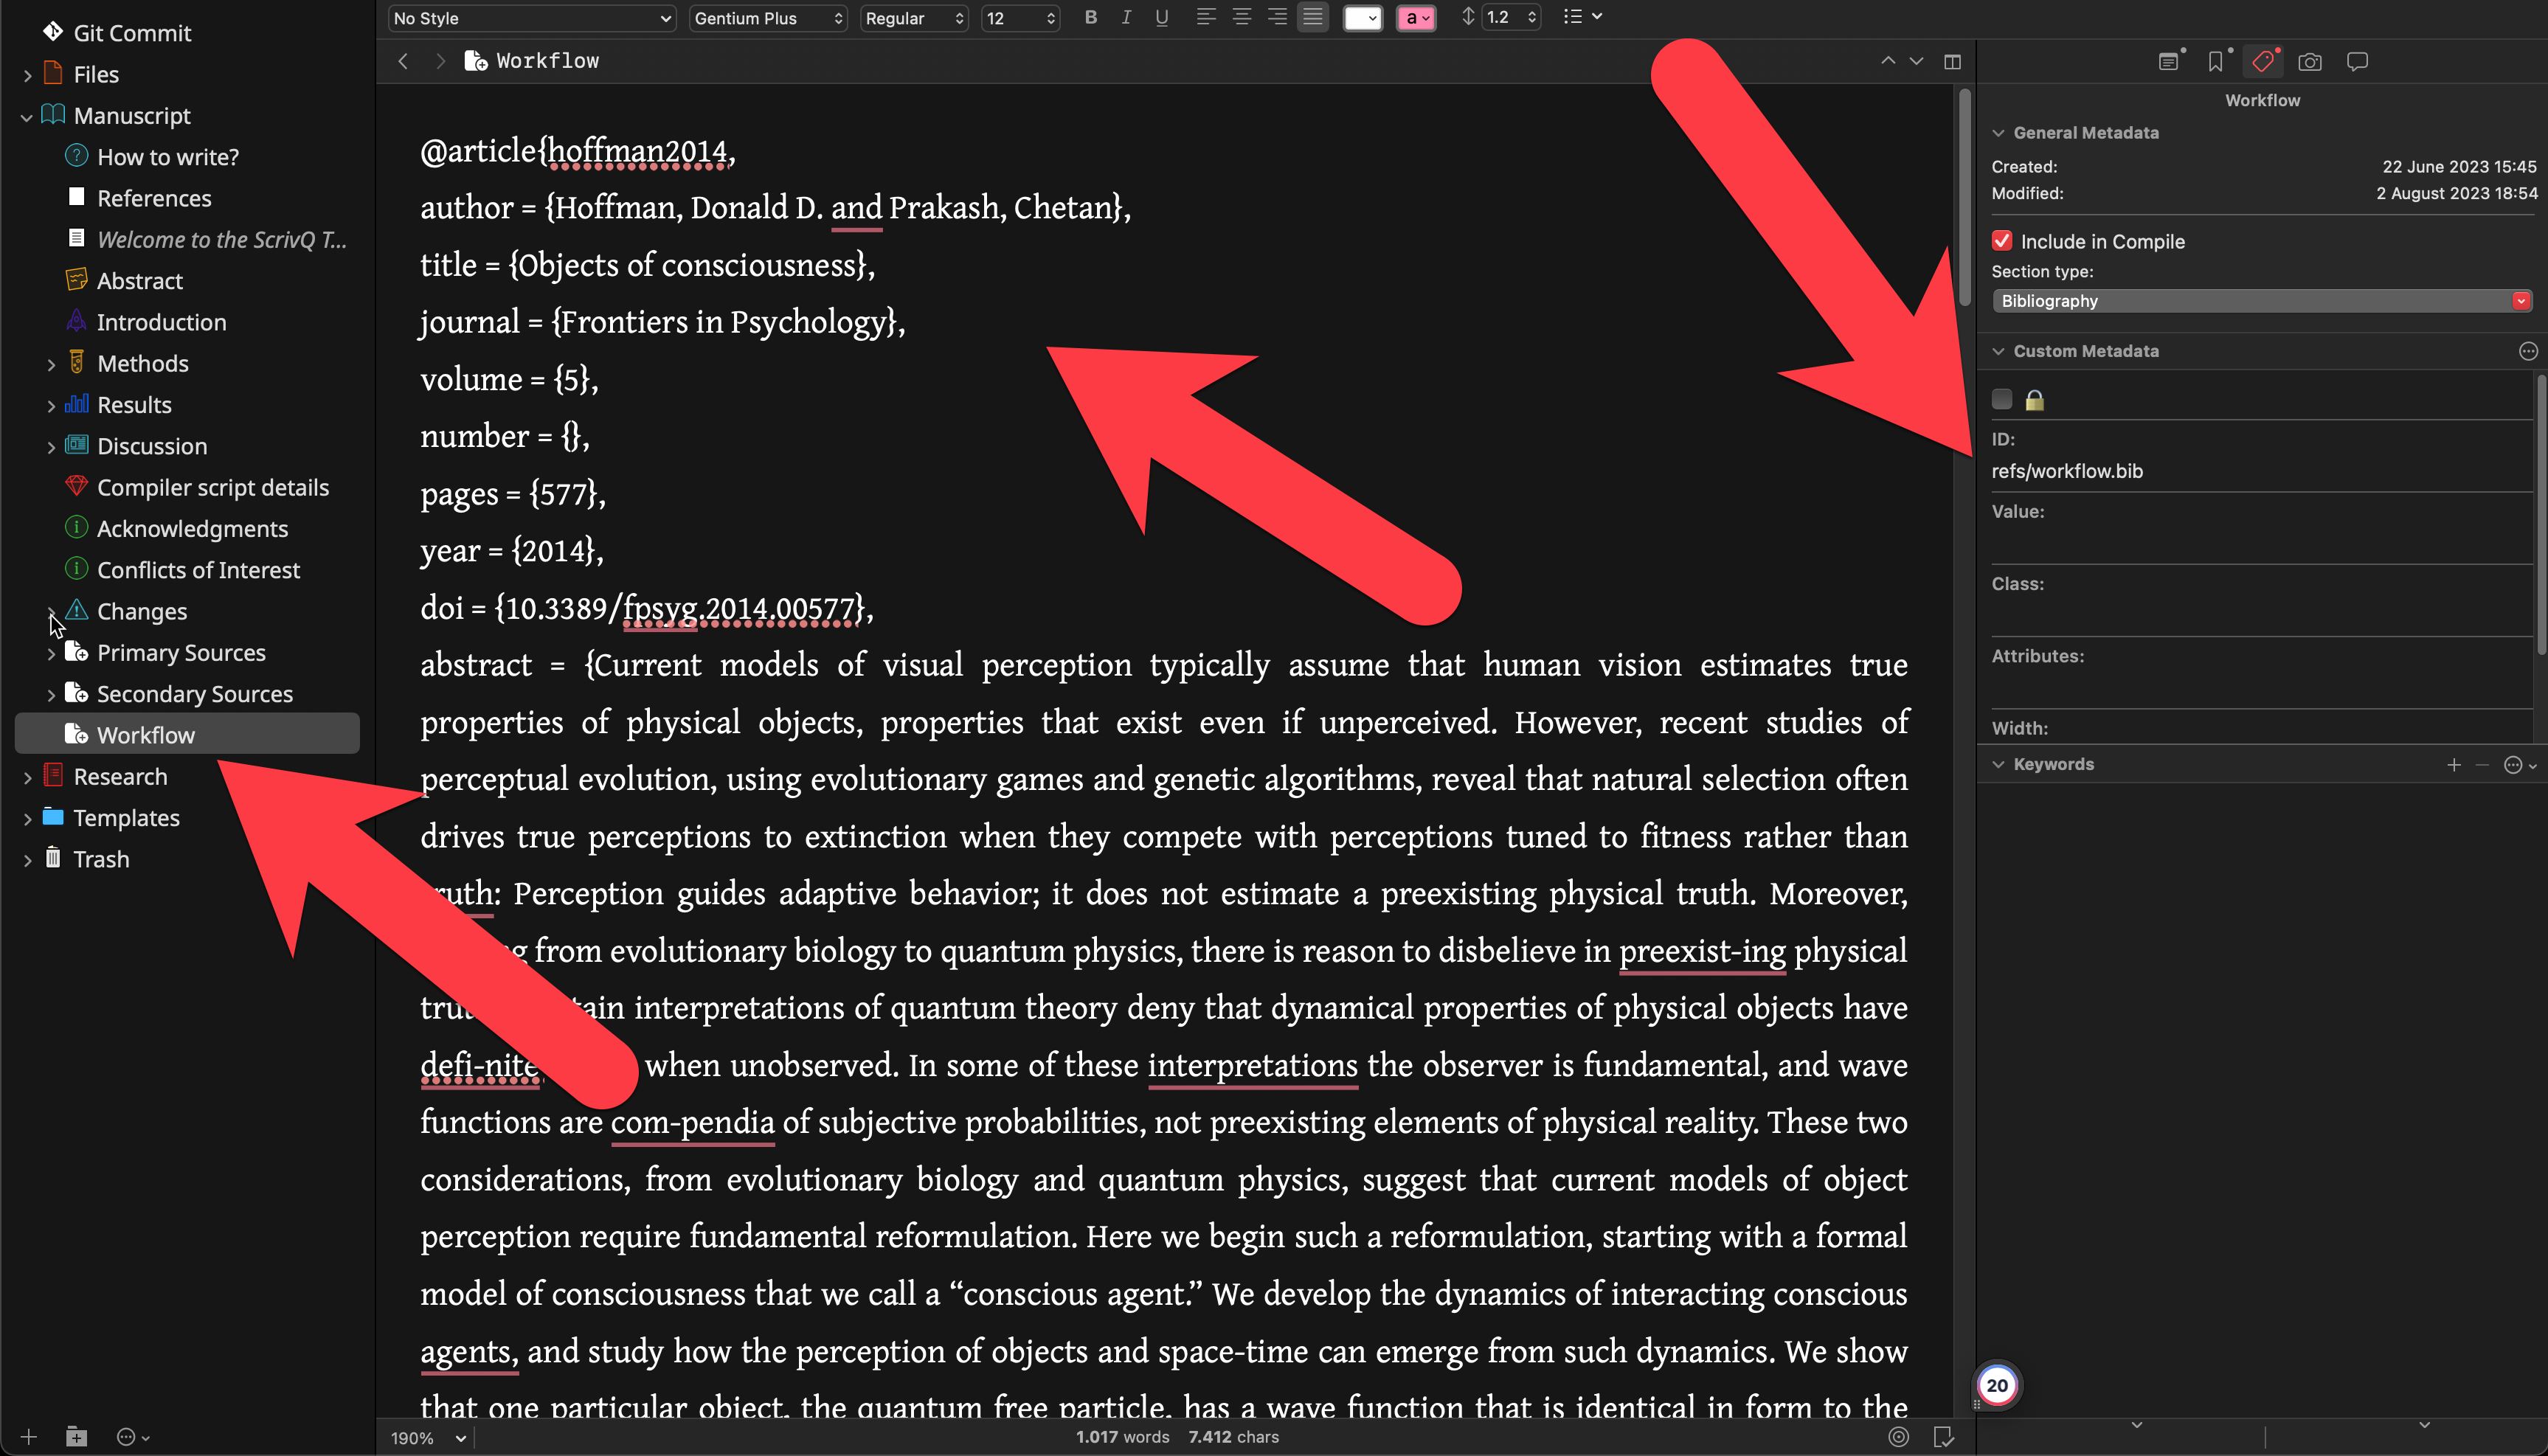
\includegraphics[width=4.02083in,height=2.30208in]{newbibliography.png}

}

\caption{\label{fig-scriv42A}This will result in a separate file, whose
path will be added to the front matter, with the content of the text.
The resulting bibliography will be printed right where we placed it in
our project.}

\end{figure}

\begin{figure}

{\centering 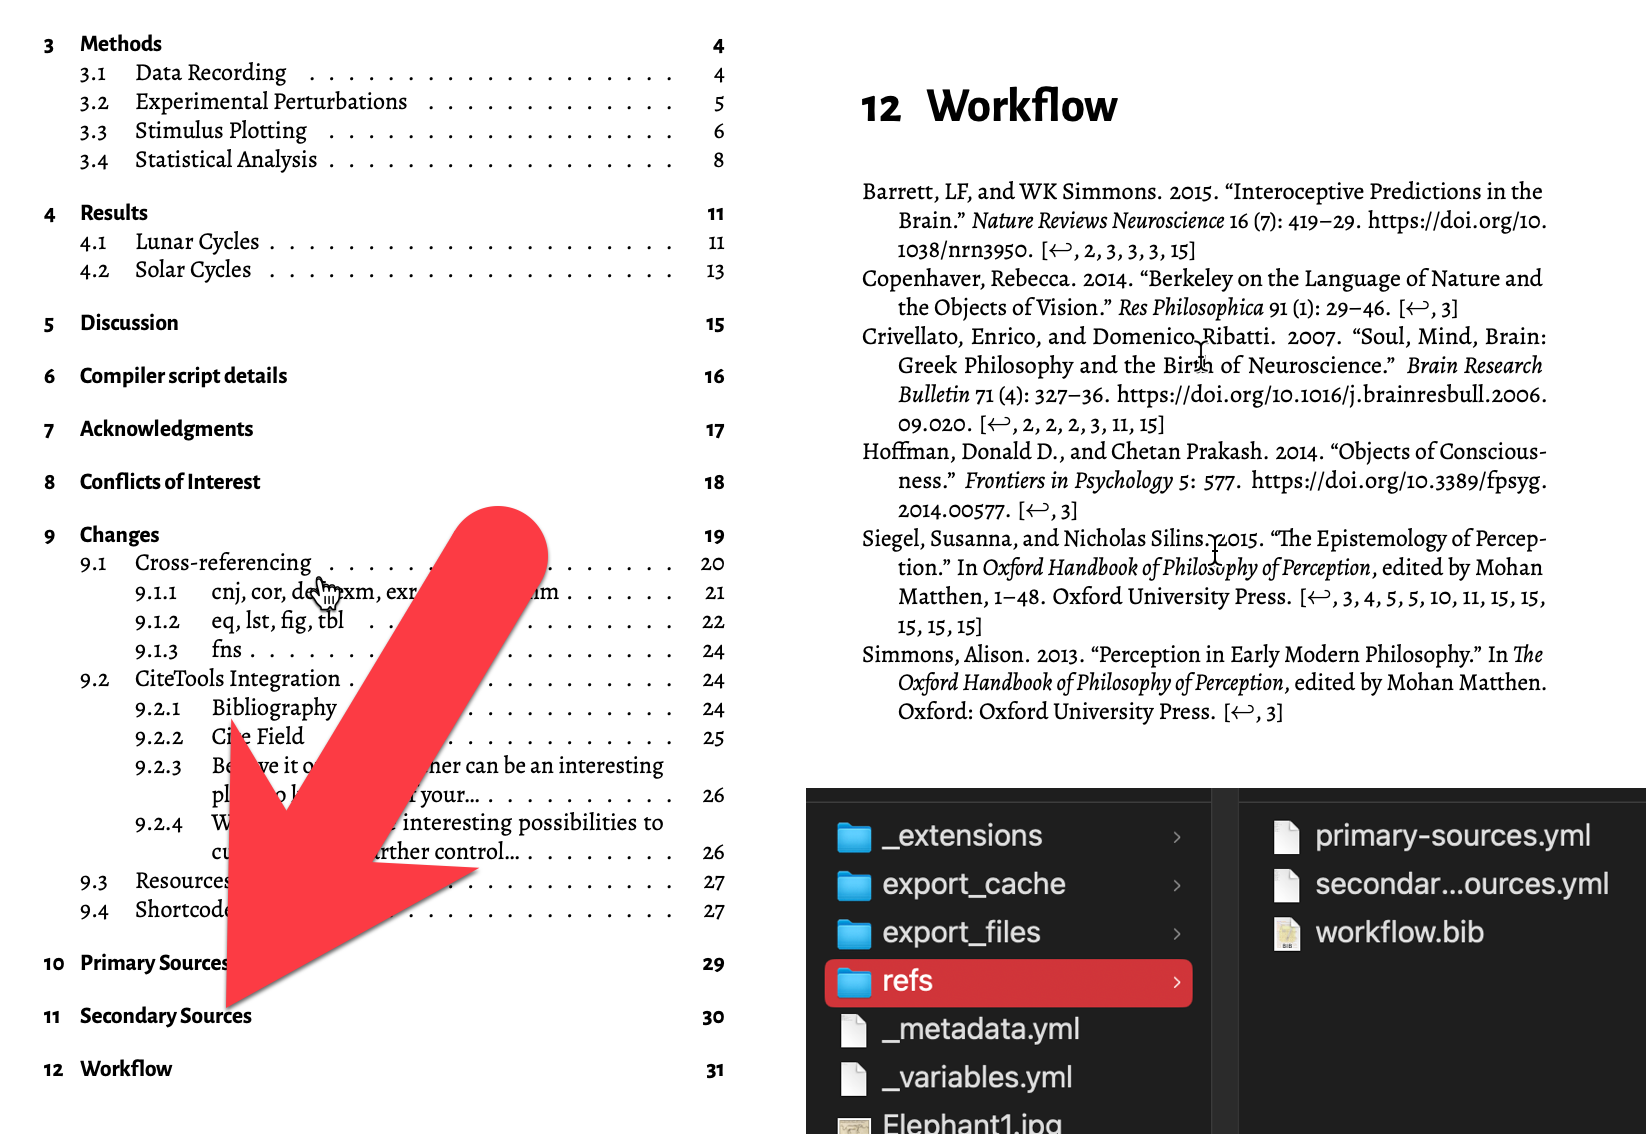
\includegraphics[width=4.45833in,height=3.07292in]{resultbib.png}

}

\caption{\label{fig-scriv42B}On the left we have the \textbf{Table of
Contents}; on the top-right, we see the printed bibliography (page 31)
and, on the bottom-right, the files are automatically created during the
compilation process.}

\end{figure}

Simply put, you can add as many bibliographies as you want!

\begin{tcolorbox}[enhanced jigsaw, rightrule=.15mm, bottomtitle=1mm, colback=white, toptitle=1mm, left=2mm, colbacktitle=quarto-callout-tip-color!10!white, opacitybacktitle=0.6, opacityback=0, arc=.35mm, leftrule=.75mm, toprule=.15mm, titlerule=0mm, breakable, coltitle=black, bottomrule=.15mm, colframe=quarto-callout-tip-color-frame, title=\textcolor{quarto-callout-tip-color}{\faLightbulb}\hspace{0.5em}{Super tip: Make use of the Templates folder}]

Thanks to \textbf{ScriQ}, there is no need to keep separate bibliography
files in the system, as the data can simply be copied and pasted from
the bibliography managers to Scrivener. However, if you already have
many bibliography files ready that you would like to use, it could be a
good idea to use the shared Templates folder to bring them to your
fingertips inside Scrivener.

\end{tcolorbox}

\begin{figure}

{\centering 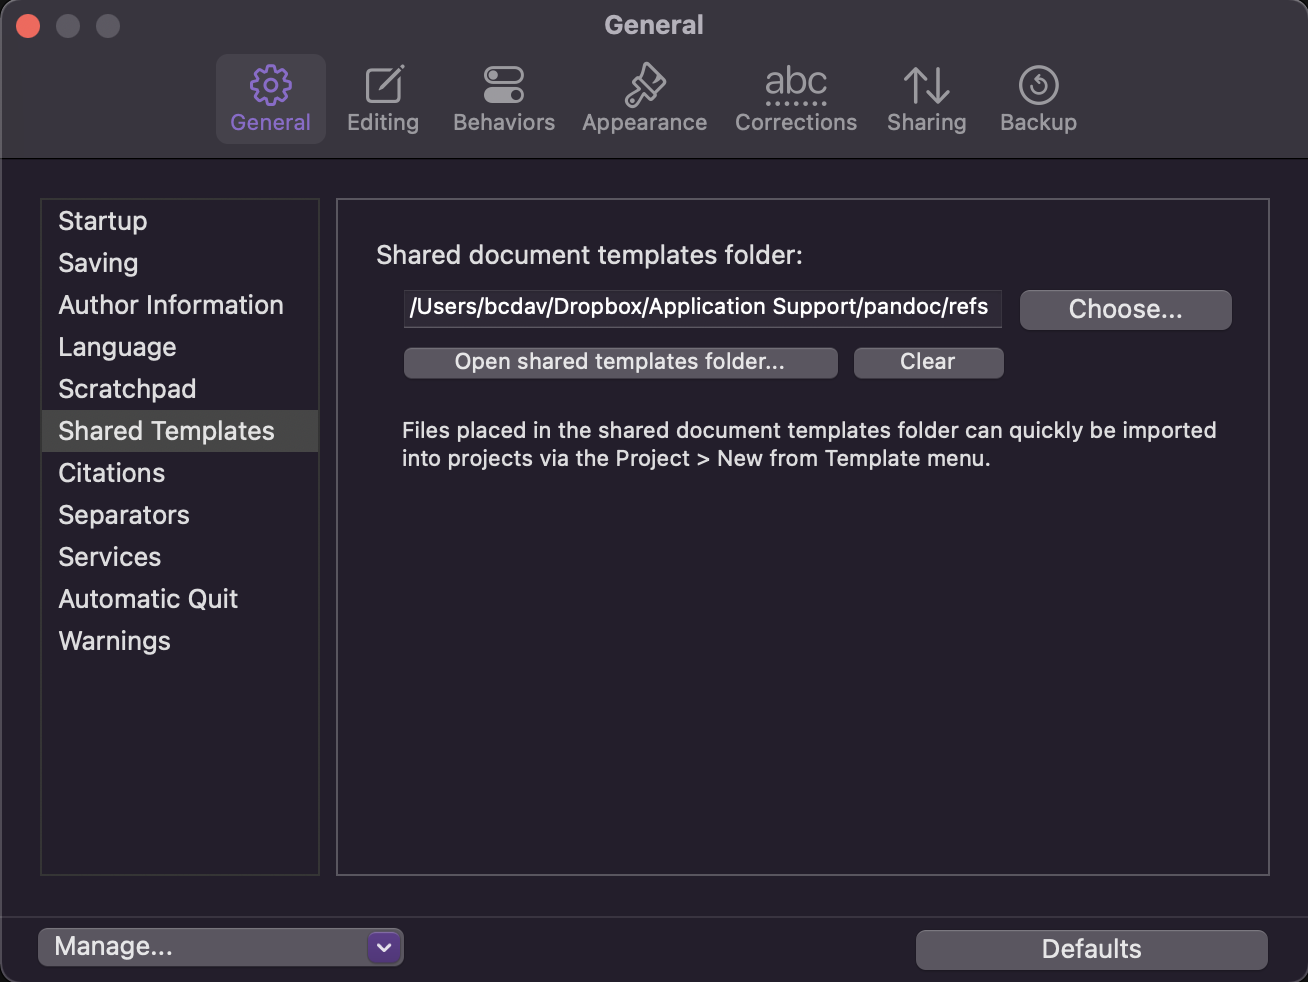
\includegraphics[width=3.11458in,height=2.34375in]{shared-templates.png}

}

\caption{\label{fig-scriv42A}The shared templates folder in the main
Scrivener configuration window.}

\end{figure}

\begin{figure}

{\centering 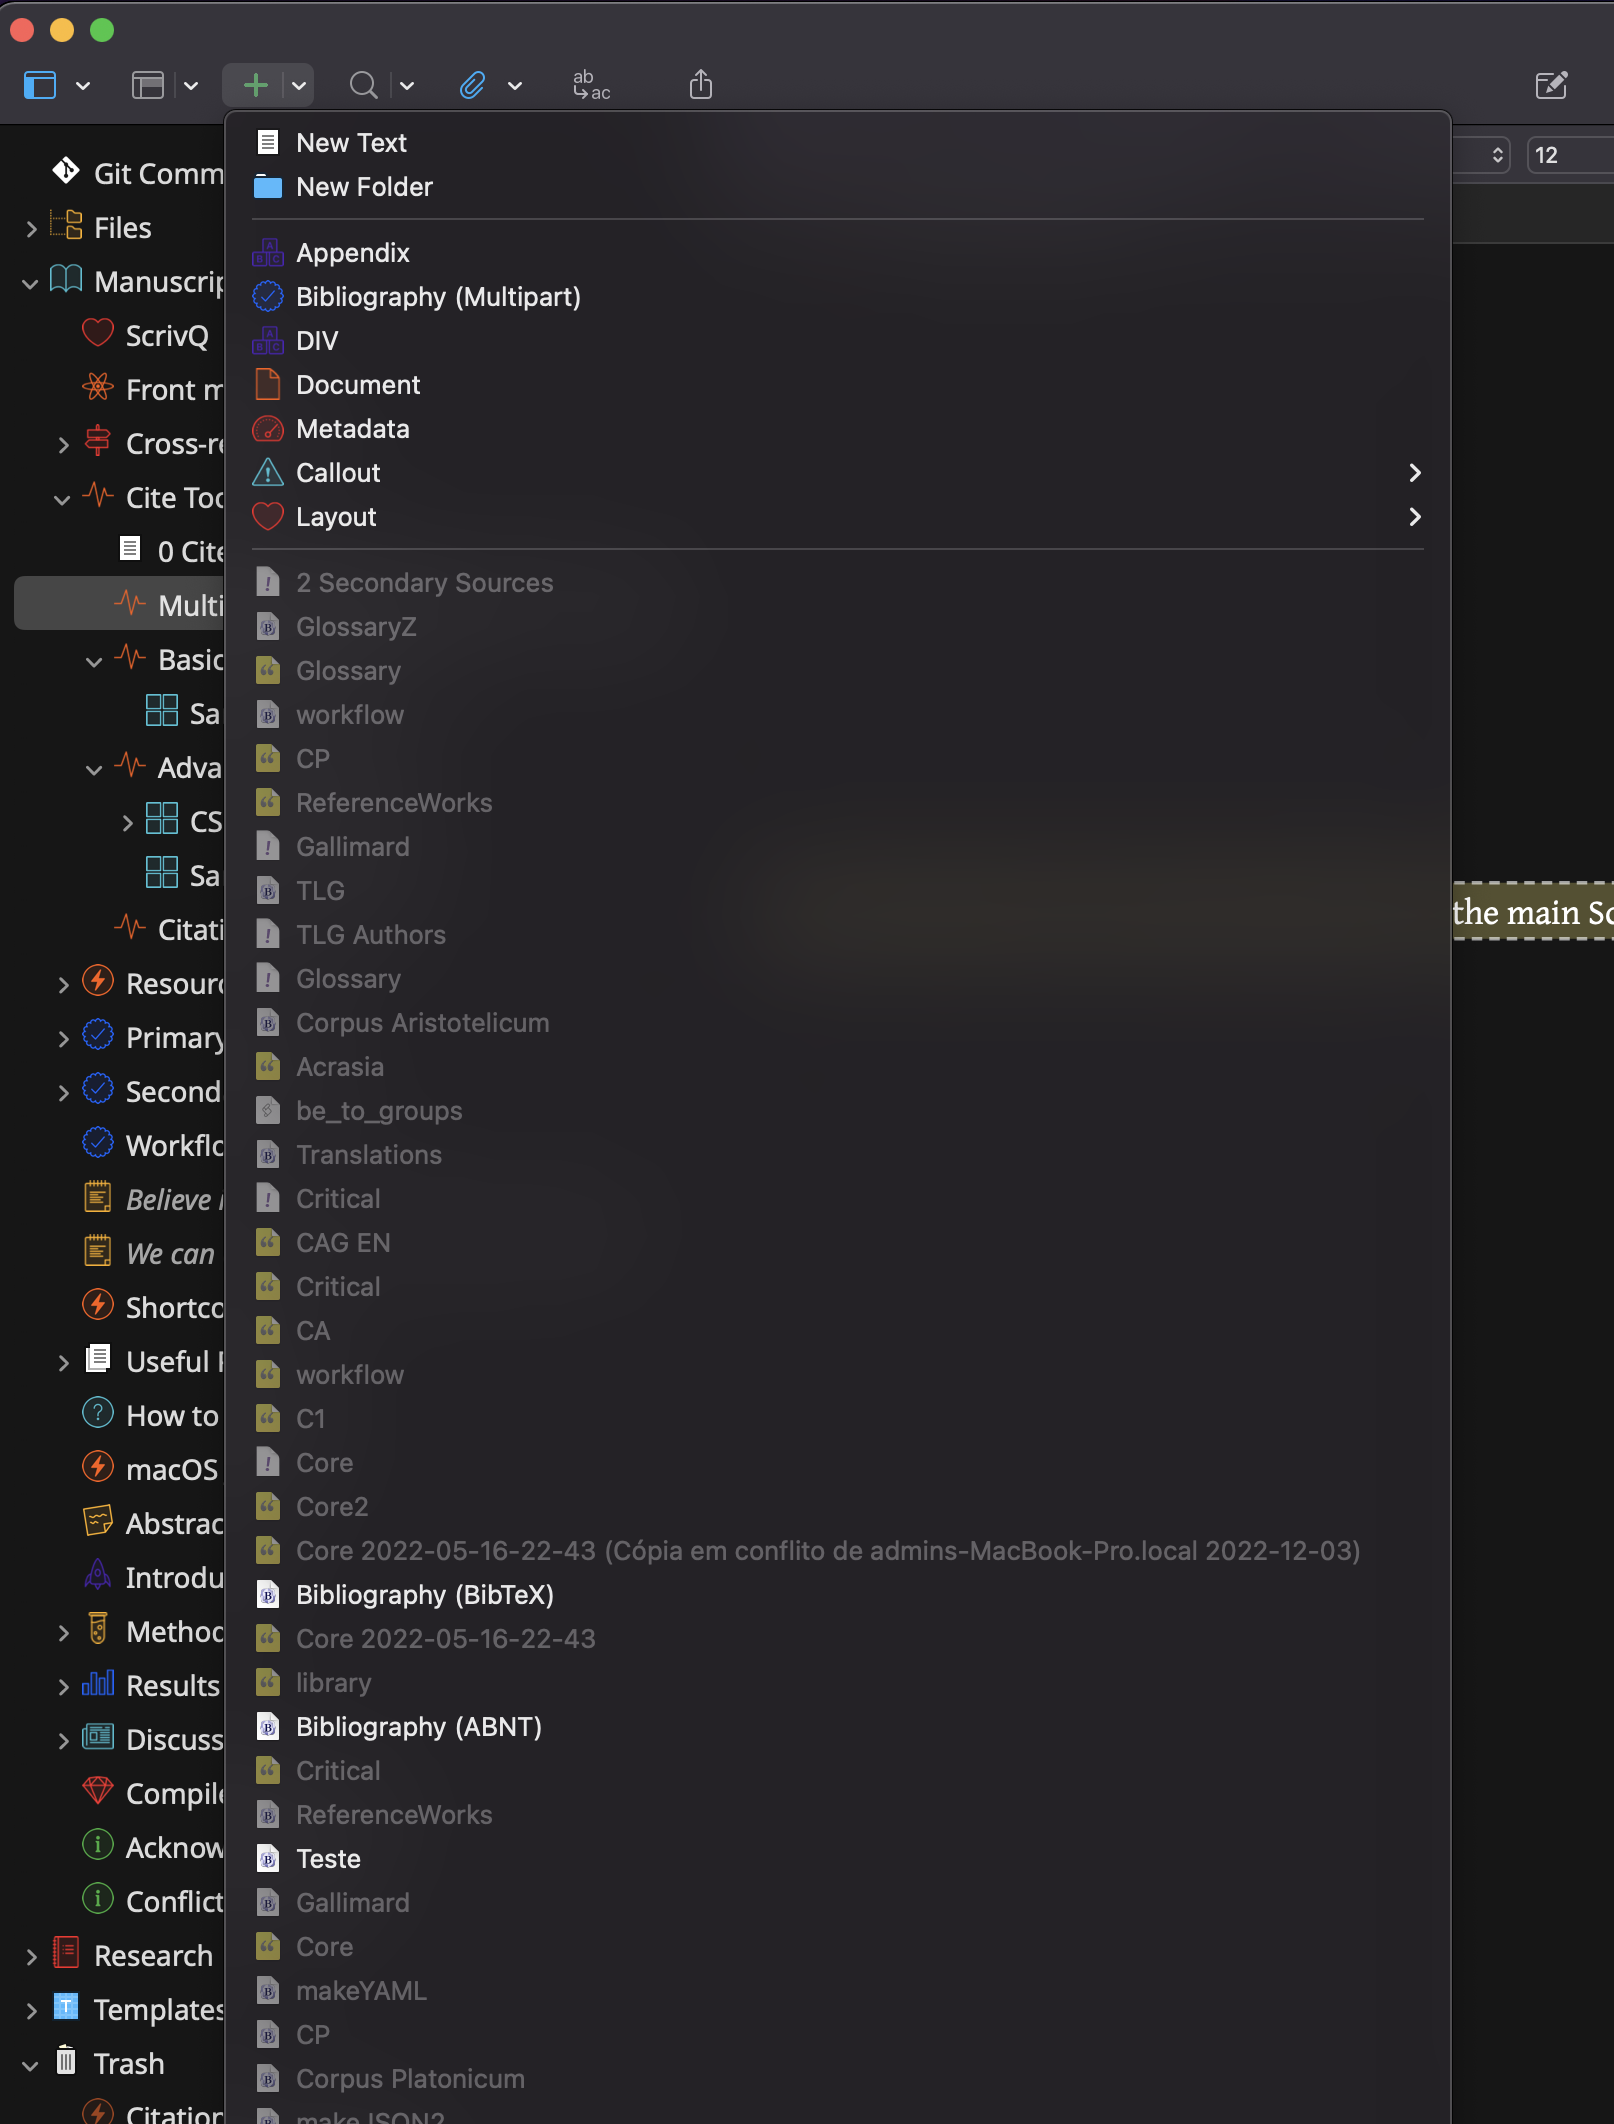
\includegraphics[width=3.0625in,height=4.03125in]{create-new-file.png}

}

\caption{\label{fig-scriv42B}The \ul{Add new document} menu in the
Toolbar.}

\end{figure}

For some reason, only \ul{.txt} files are accepted, so the files must
have this extension. Hopefully, L\&L will change this to allow other
plain text formats, such as \ul{md}, \ul{qmd}, \ul{yml}, \ul{tex},
\ul{ris}, and so on.

\begin{tcolorbox}[enhanced jigsaw, rightrule=.15mm, bottomtitle=1mm, colback=white, toptitle=1mm, left=2mm, colbacktitle=quarto-callout-note-color!10!white, opacitybacktitle=0.6, opacityback=0, arc=.35mm, leftrule=.75mm, toprule=.15mm, titlerule=0mm, breakable, coltitle=black, bottomrule=.15mm, colframe=quarto-callout-note-color-frame, title=\textcolor{quarto-callout-note-color}{\faInfo}\hspace{0.5em}{From lists of names to the formatted bibliography}]

We are feeding the bibliography data to the most natural place, that is,
precisely where it should be printed. In this case, however, we do it
using any structured format we want (\ul{bib}, \ul{ris}, \ul{yml})
unencumbered by the task of formatting the bibliography based on (some
set of) rules, which Citeproc will do for us using the provided
CSL-style file (or the default one, which is Chicago, if none is
provided).

\end{tcolorbox}

\hypertarget{sec-scriv43}{%
\section{Basic citations}\label{sec-scriv43}}

\begin{tcolorbox}[enhanced jigsaw, rightrule=.15mm, bottomtitle=1mm, colback=white, toptitle=1mm, left=2mm, colbacktitle=quarto-callout-note-color!10!white, opacitybacktitle=0.6, opacityback=0, arc=.35mm, leftrule=.75mm, toprule=.15mm, titlerule=0mm, breakable, coltitle=black, bottomrule=.15mm, colframe=quarto-callout-note-color-frame, title=\textcolor{quarto-callout-note-color}{\faInfo}\hspace{0.5em}{Official documentation}]

See the official documentation on citations at
\href{pandoc.org/MANUAL.html\#citations}{Pandoc} and
\href{quarto.org/docs/authoring/footnotes-and-citations.html\#sec-citations}{Quarto}.

\end{tcolorbox}

Let us quickly recapitulate the basics of Pandoc Citeproc and how it
uses citations.

\begin{tcolorbox}[enhanced jigsaw, rightrule=.15mm, bottomtitle=1mm, colback=white, toptitle=1mm, left=2mm, colbacktitle=quarto-callout-note-color!10!white, opacitybacktitle=0.6, opacityback=0, arc=.35mm, leftrule=.75mm, toprule=.15mm, titlerule=0mm, breakable, coltitle=black, bottomrule=.15mm, colframe=quarto-callout-note-color-frame, title=\textcolor{quarto-callout-note-color}{\faInfo}\hspace{0.5em}{Citekeys}]

As we know, each citation must have a key, composed of \texttt{@} + the
citation identifier that must begin with a letter, digit, or
\texttt{\_}, and may contain alphanumerics, \texttt{\_}, and internal
punctuation characters
(\texttt{:.\#\$\%\&-+?\textless{}\textgreater{}\textasciitilde{}/}).

\end{tcolorbox}

The citation syntax is very simple: \texttt{@Citekey} for \textbf{Author
(Date)} (an \emph{in-text} citation); \texttt{{[}@Citekey{]}} for
\textbf{(Author, Date)}; and \texttt{{[}-@Citekey{]}} for
\textbf{(Date)}. Multiple citations can be grouped in the same brackets
separated by semicolons \texttt{{[}@CitekeyA;\ @CitekeyB{]}}. The
citation key is optionally followed by a locator, which can be a page
number, a line number, a chapter number, or a section number, preceded
by a comma.

\hypertarget{tbl-scriv43}{}
\begin{longtable}[]{@{}cc@{}}
\toprule\noalign{}
\textbf{Markdown Source} & \textbf{Rendered output} \\
\midrule\noalign{}
\endfirsthead
\toprule\noalign{}
\textbf{Markdown Source} & \textbf{Rendered output} \\
\midrule\noalign{}
\endhead
\bottomrule\noalign{}
\endlastfoot
\texttt{@Long2004} & \protect\hypertarget{cite_97}{}{\label{cite_97}Long
(\protect\hyperlink{ref-Long2004}{2004})} \\
\texttt{{[}@Long2004{]}} &
\protect\hypertarget{cite_98}{}{\label{cite_98}(\protect\hyperlink{ref-Long2004}{Long
2004})} \\
\texttt{{[}@Long2004,\ p.15{]}} &
\protect\hypertarget{cite_99}{}{\label{cite_99}(\protect\hyperlink{ref-Long2004}{Long
2004, 15})} \\
\texttt{{[}-@Long2004{]}} &
\protect\hypertarget{cite_100}{}{\label{cite_100}(\protect\hyperlink{ref-Long2004}{2004})} \\
\texttt{{[}-@Long2004,\ p.15{]}} &
\protect\hypertarget{cite_101}{}{\label{cite_101}(\protect\hyperlink{ref-Long2004}{2004,
15})} \\
\caption{\label{tbl-scriv43}Citation syntax in Quarto and
Pandoc.}\tabularnewline
\end{longtable}

\begin{tcolorbox}[enhanced jigsaw, rightrule=.15mm, bottomtitle=1mm, colback=white, toptitle=1mm, left=2mm, colbacktitle=quarto-callout-note-color!10!white, opacitybacktitle=0.6, opacityback=0, arc=.35mm, leftrule=.75mm, toprule=.15mm, titlerule=0mm, breakable, coltitle=black, bottomrule=.15mm, colframe=quarto-callout-note-color-frame, title=\textcolor{quarto-callout-note-color}{\faInfo}\hspace{0.5em}{(Date)}]

\ldots on the deliberations of the prudent person
\protect\hypertarget{cite_102}{}{\label{cite_102}(\protect\hyperlink{ref-Long2004}{2004})}.

\texttt{...on\ the\ deliberations\ of\ the\ prudent\ person\ {[}-@Long2004{]}.}

\ldots on the deliberations of the prudent person
\protect\hypertarget{cite_103}{}{\label{cite_103}(\protect\hyperlink{ref-Long2004}{2004,
17})}.

\texttt{...on\ the\ deliberations\ of\ the\ prudent\ person\ {[}-@Long2004,\ p.17{]}.}

\end{tcolorbox}

\begin{tcolorbox}[enhanced jigsaw, rightrule=.15mm, bottomtitle=1mm, colback=white, toptitle=1mm, left=2mm, colbacktitle=quarto-callout-note-color!10!white, opacitybacktitle=0.6, opacityback=0, arc=.35mm, leftrule=.75mm, toprule=.15mm, titlerule=0mm, breakable, coltitle=black, bottomrule=.15mm, colframe=quarto-callout-note-color-frame, title=\textcolor{quarto-callout-note-color}{\faInfo}\hspace{0.5em}{Author (Date)}]

\protect\hypertarget{cite_104}{}{\label{cite_104}Long
(\protect\hyperlink{ref-Long2004}{2004})} says that\ldots{}

\texttt{@Long2004\ says\ that...}

\end{tcolorbox}

\begin{tcolorbox}[enhanced jigsaw, rightrule=.15mm, bottomtitle=1mm, colback=white, toptitle=1mm, left=2mm, colbacktitle=quarto-callout-note-color!10!white, opacitybacktitle=0.6, opacityback=0, arc=.35mm, leftrule=.75mm, toprule=.15mm, titlerule=0mm, breakable, coltitle=black, bottomrule=.15mm, colframe=quarto-callout-note-color-frame, title=\textcolor{quarto-callout-note-color}{\faInfo}\hspace{0.5em}{(Author, Date)}]

\ldots on the deliberations of the prudent person
\protect\hypertarget{cite_105}{}{\label{cite_105}(\protect\hyperlink{ref-Long2004}{Long
2004})}.

\texttt{...on\ the\ deliberations\ of\ the\ prudent\ person\ {[}@Long2004{]}}.

\ldots on the deliberations of the prudent person
\protect\hypertarget{cite_106}{}{\label{cite_106}(\protect\hyperlink{ref-Long2004}{Long
2004, 17})}.

\texttt{...on\ the\ deliberations\ of\ the\ prudent\ person\ {[}@Long2004,\ p.17{]}}.

\end{tcolorbox}

\begin{tcolorbox}[enhanced jigsaw, rightrule=.15mm, bottomtitle=1mm, colback=white, toptitle=1mm, left=2mm, colbacktitle=quarto-callout-note-color!10!white, opacitybacktitle=0.6, opacityback=0, arc=.35mm, leftrule=.75mm, toprule=.15mm, titlerule=0mm, breakable, coltitle=black, bottomrule=.15mm, colframe=quarto-callout-note-color-frame, title=\textcolor{quarto-callout-note-color}{\faInfo}\hspace{0.5em}{(Author, Date; Author, Date)}]

\ldots on the deliberations of the prudent person
\protect\hypertarget{cite_107}{}{\label{cite_107}(\protect\hyperlink{ref-Long2004}{Long
2004}; \protect\hyperlink{ref-hoffman2014}{Hoffman and Prakash 2014})}.

\texttt{...on\ the\ deliberations\ of\ the\ prudent\ person\ {[}@Long2004;\ @hoffman2014{]}}.

\ldots on the deliberations of the prudent person
\protect\hypertarget{cite_108}{}{\label{cite_108}(\protect\hyperlink{ref-Long2004}{Long
2004, 17}; \protect\hyperlink{ref-hoffman2014}{Hoffman and Prakash 2014,
15})}.

\texttt{...on\ the\ deliberations\ of\ the\ prudent\ person\ {[}@Long2004,\ p.17;\ @hoffman2014,\ p.15{]}.}

\end{tcolorbox}

That is pretty much all there is to it. Now that we have the basics
covered, let us see what \textbf{Cite Field} can do for us.

\hypertarget{sec-scriv44}{%
\section{Advanced citations}\label{sec-scriv44}}

\begin{tcolorbox}[enhanced jigsaw, rightrule=.15mm, bottomtitle=1mm, colback=white, toptitle=1mm, left=2mm, colbacktitle=quarto-callout-note-color!10!white, opacitybacktitle=0.6, opacityback=0, arc=.35mm, leftrule=.75mm, toprule=.15mm, titlerule=0mm, breakable, coltitle=black, bottomrule=.15mm, colframe=quarto-callout-note-color-frame, title=\textcolor{quarto-callout-note-color}{\faInfo}\hspace{0.5em}{TLDR}]

Several \textbf{Character Styles} are available to inject the correct
markup (\texttt{{[}@Citekey{]}\{.csl\_field\}}) to cite specific fields
from your references.

\end{tcolorbox}

In many areas, we are frequently invited to comment on different
editions and translations of the same classical works. In such cases, we
refer not only to the \texttt{author} and the date \texttt{issued} of a
publication, but also to its \texttt{editor}, \texttt{translator},
\texttt{publisher}, and even \texttt{original-title} and
\texttt{edition}. But how to do this? With \textbf{Cite Tools} enabled,
the answer lies in a small variation of Pandoc's vanilla syntax for
citations.

\hypertarget{tbl-scriv44}{}
\begin{longtable}[]{@{}
  >{\centering\arraybackslash}p{(\columnwidth - 4\tabcolsep) * \real{0.3333}}
  >{\centering\arraybackslash}p{(\columnwidth - 4\tabcolsep) * \real{0.3333}}
  >{\centering\arraybackslash}p{(\columnwidth - 4\tabcolsep) * \real{0.3333}}@{}}
\toprule\noalign{}
\begin{minipage}[b]{\linewidth}\centering
CSL Field
\end{minipage} & \begin{minipage}[b]{\linewidth}\centering
Markdown Source
\end{minipage} & \begin{minipage}[b]{\linewidth}\centering
Output
\end{minipage} \\
\midrule\noalign{}
\endfirsthead
\toprule\noalign{}
\begin{minipage}[b]{\linewidth}\centering
CSL Field
\end{minipage} & \begin{minipage}[b]{\linewidth}\centering
Markdown Source
\end{minipage} & \begin{minipage}[b]{\linewidth}\centering
Output
\end{minipage} \\
\midrule\noalign{}
\endhead
\bottomrule\noalign{}
\endlastfoot
Author & \texttt{{[}@DA{]}\{.author\}} & Aristotelis \\
Editor & \texttt{{[}@DA{]}\{.editor\}} & Bekker \\
Issued & \texttt{{[}@DA{]}\{.issued\}} & 1834 \\
Original-title & \texttt{{[}@DA{]}\{.original-title\}} & περὶ ψυχῆς \\
Publisher & \texttt{{[}@DA{]}\{.publisher\}} & Reimer \\
Publisher-place & \texttt{{[}@DA{]}\{.publisher-place\}} & Berlin \\
Title & \texttt{{[}@DA{]}\{.title\}} & \emph{De Anima} \\
Title-short & \texttt{{[}@DA{]}\{.title-short\}} & \emph{De An.} \\
Translator & \texttt{{[}@DA{]}\{.translator\}} & Τατάκης \\
\caption{\label{tbl-scriv44}All ready-made \textbf{Character Styles} for
the Cite Field lua filter.}\tabularnewline
\end{longtable}

As we said, internally, Pandoc uses the \textbf{C}itation \textbf{S}tyle
\textbf{L}anguage format for bibliographies. This means that \textbf{we
must use the CSL variable names} (see
\protect\hypertarget{cite_109}{}{\label{cite_109}Table~\ref{tbl-scriv50}}),
and not necessarily the field name you may see in a \textbf{RIS} or
\textbf{BibTeX} bibliography. The correct way to print the book title,
for example, would be \texttt{{[}@Citekey{]}\{.container-title\}} (and
\textbf{not} using the BibTeX alternative which is \texttt{booktitle});
likewise, the date would print with \texttt{{[}@Citekey{]}\{.issued\}},
but not with \texttt{date} or \texttt{year}.

\begin{quote}
\texttt{Aristotle\textquotesingle{}s\ {[}@DA{]}\{.original-title\}\ ({[}@DA{]}\{.title\})\ was\ first\ edited\ by\ {[}@DA{]}\{.editor\}\ in\ {[}@DA{]}\{.issued\}.\ \ In\ {[}@DABiehl{]}\{.issued\},\ there\ was\ another\ edition\ by\ {[}@DABiehl{]}\{.editor\}\ (which\ was\ reprinted\ in\ {[}@DATheiler{]}\{.translator\}\textquotesingle{}s\ {[}@DATheiler{]}\{.issued\}\ translation).}
\end{quote}

\begin{quote}
Aristotle's περὶ ψυχῆς (\emph{De Anima}) was first edited by Bekker in
1834. In 1896, there was another edition by Biehl (which was reprinted
in Theiler's 1995 translation).
\end{quote}

\hypertarget{bib-sample}{}
\begin{figure*}

\leavevmode\vadjust pre{\hypertarget{first-column}{}}%
\textbf{BibTeX}

\begin{Shaded}
\begin{Highlighting}[numbers=left,,]
\VariableTok{@book}\NormalTok{\{}\OtherTok{AristOp}\NormalTok{,}
\DataTypeTok{author}\NormalTok{ = \{Aristotle\},}
\DataTypeTok{editor}\NormalTok{ = \{Bekker, Immanuel\},}
\DataTypeTok{title}\NormalTok{ = \{Aristotelis opera\},}
\DataTypeTok{publisher}\NormalTok{ = \{Reimer\},}
\DataTypeTok{address}\NormalTok{ = \{Berlim\},}
\DataTypeTok{volumes}\NormalTok{ = \{4\},}
\DataTypeTok{edition}\NormalTok{ = \{1\},}
\DataTypeTok{year}\NormalTok{ = \{1831\}}
\NormalTok{\}}
\end{Highlighting}
\end{Shaded}

\textbf{RIS}

\begin{Shaded}
\begin{Highlighting}[numbers=left,,]
\NormalTok{TY  {-} BOOK}
\NormalTok{ID  {-} AristOp}
\NormalTok{AU  {-} Aristotle}
\NormalTok{ED  {-} Bekker, Immanuel}
\NormalTok{TI  {-} Aristotelis opera}
\NormalTok{PB  {-} Reimer}
\NormalTok{CY  {-} Berlim}
\NormalTok{ET  {-} 1}
\NormalTok{VL  {-} 4}
\NormalTok{Y1  {-} 1831}
\NormalTok{ER  {-}}
\end{Highlighting}
\end{Shaded}

\hypertarget{second-column}{}

\leavevmode\vadjust pre{\hypertarget{third-column}{}}%
\textbf{CSL-YAML}

\begin{Shaded}
\begin{Highlighting}[numbers=left,,]
\PreprocessorTok{{-}{-}{-}}
\FunctionTok{references}\KeywordTok{:}
\KeywordTok{{-}}\AttributeTok{ }\FunctionTok{author}\KeywordTok{:}
\AttributeTok{  }\KeywordTok{{-}}\AttributeTok{ }\FunctionTok{family}\KeywordTok{:}\AttributeTok{ Aristotle}
\AttributeTok{  }\FunctionTok{edition}\KeywordTok{:}\AttributeTok{ }\DecValTok{1}
\AttributeTok{  }\FunctionTok{editor}\KeywordTok{:}
\AttributeTok{  }\KeywordTok{{-}}\AttributeTok{ }\FunctionTok{family}\KeywordTok{:}\AttributeTok{ Bekker}
\AttributeTok{    }\FunctionTok{given}\KeywordTok{:}\AttributeTok{ Immanuel}
\AttributeTok{  }\FunctionTok{id}\KeywordTok{:}\AttributeTok{ AristOp}
\AttributeTok{  }\FunctionTok{issued}\KeywordTok{:}\AttributeTok{ }\DecValTok{1831}
\AttributeTok{  }\FunctionTok{number{-}of{-}volumes}\KeywordTok{:}\AttributeTok{ }\DecValTok{4}
\AttributeTok{  }\FunctionTok{publisher}\KeywordTok{:}\AttributeTok{ Reimer}
\AttributeTok{  }\FunctionTok{publisher{-}place}\KeywordTok{:}\AttributeTok{ Berlim}
\AttributeTok{  }\FunctionTok{title}\KeywordTok{:}\AttributeTok{ Aristotelis opera}
\AttributeTok{  }\FunctionTok{type}\KeywordTok{:}\AttributeTok{ book}
\PreprocessorTok{{-}{-}{-}}
\end{Highlighting}
\end{Shaded}

\end{figure*}

\hypertarget{tbl-scriv50}{}
\begin{longtable}[]{@{}
  >{\centering\arraybackslash}p{(\columnwidth - 4\tabcolsep) * \real{0.3333}}
  >{\centering\arraybackslash}p{(\columnwidth - 4\tabcolsep) * \real{0.3333}}
  >{\centering\arraybackslash}p{(\columnwidth - 4\tabcolsep) * \real{0.3333}}@{}}
\toprule\noalign{}
\begin{minipage}[b]{\linewidth}\centering
\href{https://docs.citationstyles.org/en/stable/specification.html\#appendix-iv-variables}{CSL
variables}
\end{minipage} & \begin{minipage}[b]{\linewidth}\centering
\href{https://en.wikipedia.org/wiki/BibTeX\#Field_types}{BibTeX Fields}
\end{minipage} & \begin{minipage}[b]{\linewidth}\centering
\href{https://en.wikipedia.org/wiki/RIS_(file_format)\#Tags}{RIS Tags}
\end{minipage} \\
\midrule\noalign{}
\endfirsthead
\toprule\noalign{}
\begin{minipage}[b]{\linewidth}\centering
\href{https://docs.citationstyles.org/en/stable/specification.html\#appendix-iv-variables}{CSL
variables}
\end{minipage} & \begin{minipage}[b]{\linewidth}\centering
\href{https://en.wikipedia.org/wiki/BibTeX\#Field_types}{BibTeX Fields}
\end{minipage} & \begin{minipage}[b]{\linewidth}\centering
\href{https://en.wikipedia.org/wiki/RIS_(file_format)\#Tags}{RIS Tags}
\end{minipage} \\
\midrule\noalign{}
\endhead
\bottomrule\noalign{}
\endlastfoot
abstract & abstract & AB \\
author & authors & AU A1 \\
call-number & library & ID \\
chapter-number collection-number number issue & chapter number issue &
IS \\
collection-title & series & - \\
container-title & booktitle journal & BT T2 JA JF JO \\
DOI & doi & DO \\
editor & editors & A2 ED \\
genre & type & - \\
ISSN & issn & SN \\
issued & date & PY Y1 \\
keywords & keywords & KW \\
language & langid & LA \\
number-of-volumes & volumes & NV \\
original-title & origtitle & OR* \\
page & pages & SP EP \\
publisher & publisher school institution organization howpublished &
PB \\
publisher-place & address & PP \\
title & title & TI T1 CT \\
title-short & shorttitle & ST* \\
url & URL & UR LK \\
version & version & - \\
volume & volume & VL \\
\caption{\label{tbl-scriv50}CSL-YAML/CSL-JSON variables alongside
corresponding
\href{https://github.com/jgm/pandoc/blob/main/src/Text/Pandoc/Citeproc/BibTeX.hs}{BibTeX}
fields and
\href{https://github.com/jgm/pandoc/blob/main/src/Text/Pandoc/Readers/RIS.hs}{RIS}
tags. Those marked with an asterisk exist and correspond, but, for some
reason, Pandoc ignores them instead of converting to
CSL.}\tabularnewline
\end{longtable}

\hypertarget{sec-scriv51}{%
\section{Citation Backlinks}\label{sec-scriv51}}

With Pandoc Citeproc, you can use \texttt{link-citations} to control
whether citations in the body of the text should be clickable links to
the reference in the bibliography (e.g.~\texttt{{[}@EN{]}}). This is a
very useful feature, especially when you want to quickly check the
source of a citation without having to scroll through the whole text.
\textbf{ScrivQ} takes this one step further with \textbf{Cite Tools} and
adds, in a crescent ordinal fashion\footnote{In other output formats,
  such as PDF, the reader will see the page number instead of a crescent
  ordinal number.}, a backlink to each citation an entry has received in
the document. This allows the reader to easily arrive at sections of the
text where the same reference was discussed, quickly seeing with the
array of backlinks, how many times each reference was used in the text.

\begin{tcolorbox}[enhanced jigsaw, rightrule=.15mm, bottomtitle=1mm, colback=white, toptitle=1mm, left=2mm, colbacktitle=quarto-callout-warning-color!10!white, opacitybacktitle=0.6, opacityback=0, arc=.35mm, leftrule=.75mm, toprule=.15mm, titlerule=0mm, breakable, coltitle=black, bottomrule=.15mm, colframe=quarto-callout-warning-color-frame, title=\textcolor{quarto-callout-warning-color}{\faExclamationTriangle}\hspace{0.5em}{Turning off undesired linking}]

You can set \texttt{link-fields} to false to avoid undesired linking
when citing specific fields
(\protect\hypertarget{cite_110}{}{\label{cite_110}Section~\ref{sec-scriv44}}).

\end{tcolorbox}

\begin{tcolorbox}[enhanced jigsaw, rightrule=.15mm, opacityback=0, arc=.35mm, colback=white, toprule=.15mm, breakable, bottomrule=.15mm, left=2mm, colframe=quarto-callout-tip-color-frame, leftrule=.75mm]
\begin{minipage}[t]{5.5mm}
\textcolor{quarto-callout-tip-color}{\faLightbulb}
\end{minipage}%
\begin{minipage}[t]{\textwidth - 5.5mm}

\textbf{Various parameters that affect the hyperlinking of the
bibliography}\vspace{2mm}

\ul{link-citations}: Hyperlink citations to the corresponding
bibliography entries. Defaults to false.

\ul{link-fields}: Hyperlink citations that target specific CSL fields to
the corresponding entries in the bibliography. If link-citations is
true, this defaults to true.

\ul{link-bibliography}: Hyperlink DOIs, PMCIDs, PMID, and URLs in
bibliographies. Defaults to true.

\ul{lang}: Affects the bibliography tags. Defaults to \texttt{en-US}.

\end{minipage}%
\end{tcolorbox}

\hypertarget{sec-scriv52}{%
\chapter{Resources}\label{sec-scriv52}}

There are several other incredible resources in ScrivQ. Seriously. I
spent easily over one hundred hours building this template, adding
useful, good, and pretty things to it (aren't the icons lovely?). There
are still many undocumented developed features that will receive proper
treatment in upcoming versions. Just to mention in passing, the next
step will probably be documenting some of the already existing
possibilities for editing Pandoc templates inside Scrivener. This is
already possible and being done, (everything is there and it is already
working).

\begin{itemize}
\tightlist
\item
  Bootstrap Icons - https://icons.getbootstrap.com - These are available
  in Quarto documents using the \textbf{Shortcode Font Awesome} style as
  in \texttt{} . (There is also \textbf{Shortcode Env},
  \textbf{Shortcode Meta}, \textbf{Shortcode Var}).
\item
  Writing in Scrivener
  (https://github.com/iandol/scrivomatic\#writing-in-scrivener) is a
  must read.
\item
  The Plain Person's Guide to Plain Text Social Science -
  https://plain-text.co/index.html\#introduction
\item
  Quarto Reference - https://quarto.org/docs/reference/
\item
  The easiest way to publish to Github Pages: Render to docs
\item
  Example of Quarto Book -
  https://github.com/jjallaire/hopr/blob/master/\_quarto.yml
\item
  Quarto with GH Pages - https://tarleb.com/posts/quarto-with-gh-pages/
\end{itemize}

\hypertarget{sec-scriv53}{%
\section{Callout}\label{sec-scriv53}}

These sections are divs with hardcoded classes (.callout-caution,
.callout-important, .callout-note, .callout-tip, .callout-warning).

\begin{tcolorbox}[enhanced jigsaw, rightrule=.15mm, opacityback=0, arc=.35mm, colback=white, toprule=.15mm, breakable, bottomrule=.15mm, left=2mm, colframe=quarto-callout-caution-color-frame, leftrule=.75mm]
\begin{minipage}[t]{5.5mm}
\textcolor{quarto-callout-caution-color}{\faFire}
\end{minipage}%
\begin{minipage}[t]{\textwidth - 5.5mm}

\textbf{Callout Caution}\vspace{2mm}

\end{minipage}%
\end{tcolorbox}

\begin{tcolorbox}[enhanced jigsaw, rightrule=.15mm, opacityback=0, arc=.35mm, colback=white, toprule=.15mm, breakable, bottomrule=.15mm, left=2mm, colframe=quarto-callout-important-color-frame, leftrule=.75mm]
\begin{minipage}[t]{5.5mm}
\textcolor{quarto-callout-important-color}{\faExclamation}
\end{minipage}%
\begin{minipage}[t]{\textwidth - 5.5mm}

\textbf{Callout Important}\vspace{2mm}

\end{minipage}%
\end{tcolorbox}

\begin{tcolorbox}[enhanced jigsaw, rightrule=.15mm, opacityback=0, arc=.35mm, colback=white, toprule=.15mm, breakable, bottomrule=.15mm, left=2mm, colframe=quarto-callout-note-color-frame, leftrule=.75mm]
\begin{minipage}[t]{5.5mm}
\textcolor{quarto-callout-note-color}{\faInfo}
\end{minipage}%
\begin{minipage}[t]{\textwidth - 5.5mm}

\textbf{Callout Note}\vspace{2mm}

\end{minipage}%
\end{tcolorbox}

\begin{tcolorbox}[enhanced jigsaw, rightrule=.15mm, opacityback=0, arc=.35mm, colback=white, toprule=.15mm, breakable, bottomrule=.15mm, left=2mm, colframe=quarto-callout-tip-color-frame, leftrule=.75mm]
\begin{minipage}[t]{5.5mm}
\textcolor{quarto-callout-tip-color}{\faLightbulb}
\end{minipage}%
\begin{minipage}[t]{\textwidth - 5.5mm}

\textbf{Callout Tip}\vspace{2mm}

\end{minipage}%
\end{tcolorbox}

\begin{tcolorbox}[enhanced jigsaw, rightrule=.15mm, opacityback=0, arc=.35mm, colback=white, toprule=.15mm, breakable, bottomrule=.15mm, left=2mm, colframe=quarto-callout-warning-color-frame, leftrule=.75mm]
\begin{minipage}[t]{5.5mm}
\textcolor{quarto-callout-warning-color}{\faExclamationTriangle}
\end{minipage}%
\begin{minipage}[t]{\textwidth - 5.5mm}

\textbf{Callout Warning}\vspace{2mm}

\end{minipage}%
\end{tcolorbox}

\hypertarget{sec-scriv59}{%
\section{Layout}\label{sec-scriv59}}

\hypertarget{scriv60}{}
\begin{figure*}

The \textbf{Section Type }{[}\texttt{Column\ Page}{]} adds the
homonymous class to make the content much wider, though stopping short
of extending across the whole document. See
https://quarto.org/docs/authoring/article-layout.html for details. Lorem
ipsum dolor sit amet, consectetur adipisicing elit, sed do eiusmod
tempor incididunt ut labore et dolore magna aliqua. Ut enim ad minim
veniam, quis nostrud exercitation ullamco laboris nisi ut aliquip ex ea
commodo consequat.

\end{figure*}

\hypertarget{scriv61}{}
\begin{figure*}

The contents will be assigned the \texttt{.column-page-right} class and
stretched rightwards across the page, see
https://quarto.org/docs/authoring/article-layout.html for details. Lorem
ipsum dolor sit amet, consectetur adipisicing elit, sed do eiusmod
tempor incididunt ut labore et dolore magna aliqua.

\end{figure*}

\leavevmode\vadjust pre{\hypertarget{scriv62}{}}%
The contents will be assigned the \texttt{.column-page-left} class and
stretched leftwards across the page, see
https://quarto.org/docs/authoring/article-layout.html for details.

\hypertarget{scriv63}{}
\begin{figure*}

This is an example of the \texttt{Column\ Screen} section type. Lorem
ipsum dolor sit amet, consectetur adipisicing elit, sed do eiusmod
tempor incididunt ut labore et dolore magna aliqua.

\end{figure*}

\hypertarget{scriv64}{}
\marginnote{\begin{footnotesize}

This Marginalia is using a Section Type {[}\texttt{Column\ Margin}{]}.
The contents will be assigned the \texttt{.column-margin} class and
placed in the margin in HTML and LaTeX outputs. See
https://quarto.org/docs/authoring/article-layout.html for
details\ldots{}

\end{footnotesize}}

\hypertarget{sec-scriv65}{%
\section{Generic Divs}\label{sec-scriv65}}

Finally, we'll look at how we can use generic \ul{Div} sections to
recreate some of the other hardcoded sections.

Some people might understandably prefer to achieve with fewer
\textbf{Section Types} the same functionalities afforded by the
profusion we saw earlier. To give an example, all Amsthm
(\protect\hypertarget{cite_111}{}{\label{cite_111}Section~\ref{sec-scriv4}})
elements, the Multipart panels
(\protect\hypertarget{cite_112}{}{\label{cite_112}Section~\ref{sec-scriv21}},
\protect\hypertarget{cite_113}{}{\label{cite_113}Section~\ref{sec-scriv29}}),
the Callouts
(\protect\hypertarget{cite_114}{}{\label{cite_114}Section~\ref{sec-scriv53}}),
and the Column Layouts
(\protect\hypertarget{cite_115}{}{\label{cite_115}Section~\ref{sec-scriv59}})
could be created from a single generic Div section. This is even made
easier by the presence of the \textless\$custom:ID-Prefix\textgreater,
\textless\$custom:Class\textgreater, and
\textless\$custom:Class₂\textgreater{} fields, which unencumbers the
user from remembering the correct prefix for \textbf{Amsthm} or
\textbf{Cross-reference} sections, and the classes for \textbf{Callouts}
and different \textbf{Column Layout} options.

\begin{tcolorbox}[enhanced jigsaw, rightrule=.15mm, bottomtitle=1mm, colback=white, toptitle=1mm, left=2mm, colbacktitle=quarto-callout-tip-color!10!white, opacitybacktitle=0.6, opacityback=0, arc=.35mm, leftrule=.75mm, toprule=.15mm, titlerule=0mm, breakable, coltitle=black, bottomrule=.15mm, colframe=quarto-callout-tip-color-frame, title=\textcolor{quarto-callout-tip-color}{\faLightbulb}\hspace{0.5em}{Tip}]

For \ul{\textless\$custom:Width\textgreater{}} and
\ul{\textless\$custom:Height\textgreater{}}, you can input the value
\emph{directly}. There is no need to add \texttt{width=} or place the
value between quotes. This will automatically be done for you.

\end{tcolorbox}

\begin{tcolorbox}[enhanced jigsaw, rightrule=.15mm, bottomtitle=1mm, colback=white, toptitle=1mm, left=2mm, colbacktitle=quarto-callout-note-color!10!white, opacitybacktitle=0.6, opacityback=0, arc=.35mm, leftrule=.75mm, toprule=.15mm, titlerule=0mm, breakable, coltitle=black, bottomrule=.15mm, colframe=quarto-callout-note-color-frame, title=\textcolor{quarto-callout-note-color}{\faInfo}\hspace{0.5em}{Note}]

If the fields are left empty, the ruby script will remove the empty keys
for us.

\end{tcolorbox}

\newpage{}

\hypertarget{sec-scriv68}{%
\chapter{Final word}\label{sec-scriv68}}

Now that you have familiarized yourself with \textbf{ScrivQ}, I ask you
to consider the following: this template was developed not by ChatGPT,
or some other automated method, but by \emph{an obscene amount of time
and effort} from a real human being. So, ask yourself, \enquote{How much
is it worth to me to employ this in my work?}, \enquote{How much is it
worth it to me to always have an updated working version?}. Then,
\href{https://github.com/sponsors/bcdavasconcelos}{I ask you to let the
artisan know}. It makes a big difference. Thanks for reading!

\hypertarget{sec-scriv69}{%
\chapter{References}\label{sec-scriv69}}

\hypertarget{sec-scriv70}{%
\section{Primary Sources}\label{sec-scriv70}}

\hypertarget{refs_scriv70}{}
\begin{CSLReferences}{1}{0}
\leavevmode\vadjust pre{\hypertarget{ref-DA}{}}%
Aristotelis. 1834. {``De Anima.''} In \emph{Aristotelis Opera}, edited
by Immanuel Bekker, translated by Β. Τατάκης. Berlin: Reimer.
{[}\Acrobatmenu{GoBack}{$\hookleftarrow$}{]}

\leavevmode\vadjust pre{\hypertarget{ref-Men}{}}%
Plato. 1903. \emph{Meno}. Edited by John Burnet. \emph{Platonis Opera}.
Oxford: OCT. {[}\Acrobatmenu{GoBack}{$\hookleftarrow$}{]}

\end{CSLReferences}

\hypertarget{sec-scriv117}{%
\section{Secondary Sources}\label{sec-scriv117}}

\hypertarget{refs_scriv117}{}
\begin{CSLReferences}{1}{0}
\leavevmode\vadjust pre{\hypertarget{ref-DABiehl}{}}%
Aristotelis. 1896. \emph{De Anima}. Edited by Wilhelm Biehl. Leipzig:
Teubner. {[}\Acrobatmenu{GoBack}{$\hookleftarrow$}{]}

\leavevmode\vadjust pre{\hypertarget{ref-DATheiler}{}}%
---------. 1995. \emph{De Anima}. Edited by Wilhelm Biehl. Translated by
Willy Theiler and Horst Seidl. Harmburg: Felix Meiner.
{[}\Acrobatmenu{GoBack}{$\hookleftarrow$}{]}

\leavevmode\vadjust pre{\hypertarget{ref-Long2004}{}}%
Long, Christopher. 2004. \emph{Ethics of Ontology}. SUNY Series in
Ancient Greek Philosophy. Albany: SUNY.
{[}\Acrobatmenu{GoBack}{$\hookleftarrow$},
\protect\hyperlink{cite_97}{\pageref{cite_97}},
\protect\hyperlink{cite_98}{\pageref{cite_98}},
\protect\hyperlink{cite_99}{\pageref{cite_99}},
\protect\hyperlink{cite_100}{\pageref{cite_100}},
\protect\hyperlink{cite_101}{\pageref{cite_101}},
\protect\hyperlink{cite_102}{\pageref{cite_102}},
\protect\hyperlink{cite_103}{\pageref{cite_103}},
\protect\hyperlink{cite_104}{\pageref{cite_104}},
\protect\hyperlink{cite_105}{\pageref{cite_105}},
\protect\hyperlink{cite_106}{\pageref{cite_106}},
\protect\hyperlink{cite_107}{\pageref{cite_107}},
\protect\hyperlink{cite_108}{\pageref{cite_108}}{]}

\end{CSLReferences}

\hypertarget{sec-scriv163}{%
\section{Workflow}\label{sec-scriv163}}

\hypertarget{refs_scriv163}{}
\begin{CSLReferences}{1}{0}
\leavevmode\vadjust pre{\hypertarget{ref-hoffman2014}{}}%
Hoffman, Donald D., and Chetan Prakash. 2014. {``Objects of
Consciousness.''} \emph{Frontiers in Psychology} 5: 577.
\url{https://doi.org/10.3389/fpsyg.2014.00577}.
{[}\Acrobatmenu{GoBack}{$\hookleftarrow$},
\protect\hyperlink{cite_107}{\pageref{cite_107}},
\protect\hyperlink{cite_108}{\pageref{cite_108}}{]}

\end{CSLReferences}

\hypertarget{sec-scriv164}{%
\section{Songs}\label{sec-scriv164}}

\hypertarget{refs_scriv164}{}
\begin{CSLReferences}{1}{0}
\leavevmode\vadjust pre{\hypertarget{ref-MorphineCFP}{}}%
Morphine, Mark Sandman, Dana Colley, and Jerome Deupree. 1993.
\emph{Cure For Pain}. CD. Cure For Pain. Rykodisc.
\url{https://open.spotify.com/track/3hO9gaVixKDoYDrlTBrEWf?si=0668baf1aab345d4}.
{[}\Acrobatmenu{GoBack}{$\hookleftarrow$}{]}

\end{CSLReferences}

\hypertarget{sec-scriv165}{%
\chapter*{Cite Tools Samples}\label{sec-scriv165}}
\addcontentsline{toc}{chapter}{Cite Tools Samples}

\protect\hypertarget{scriv165}{}{}

\begin{figure}

{\centering 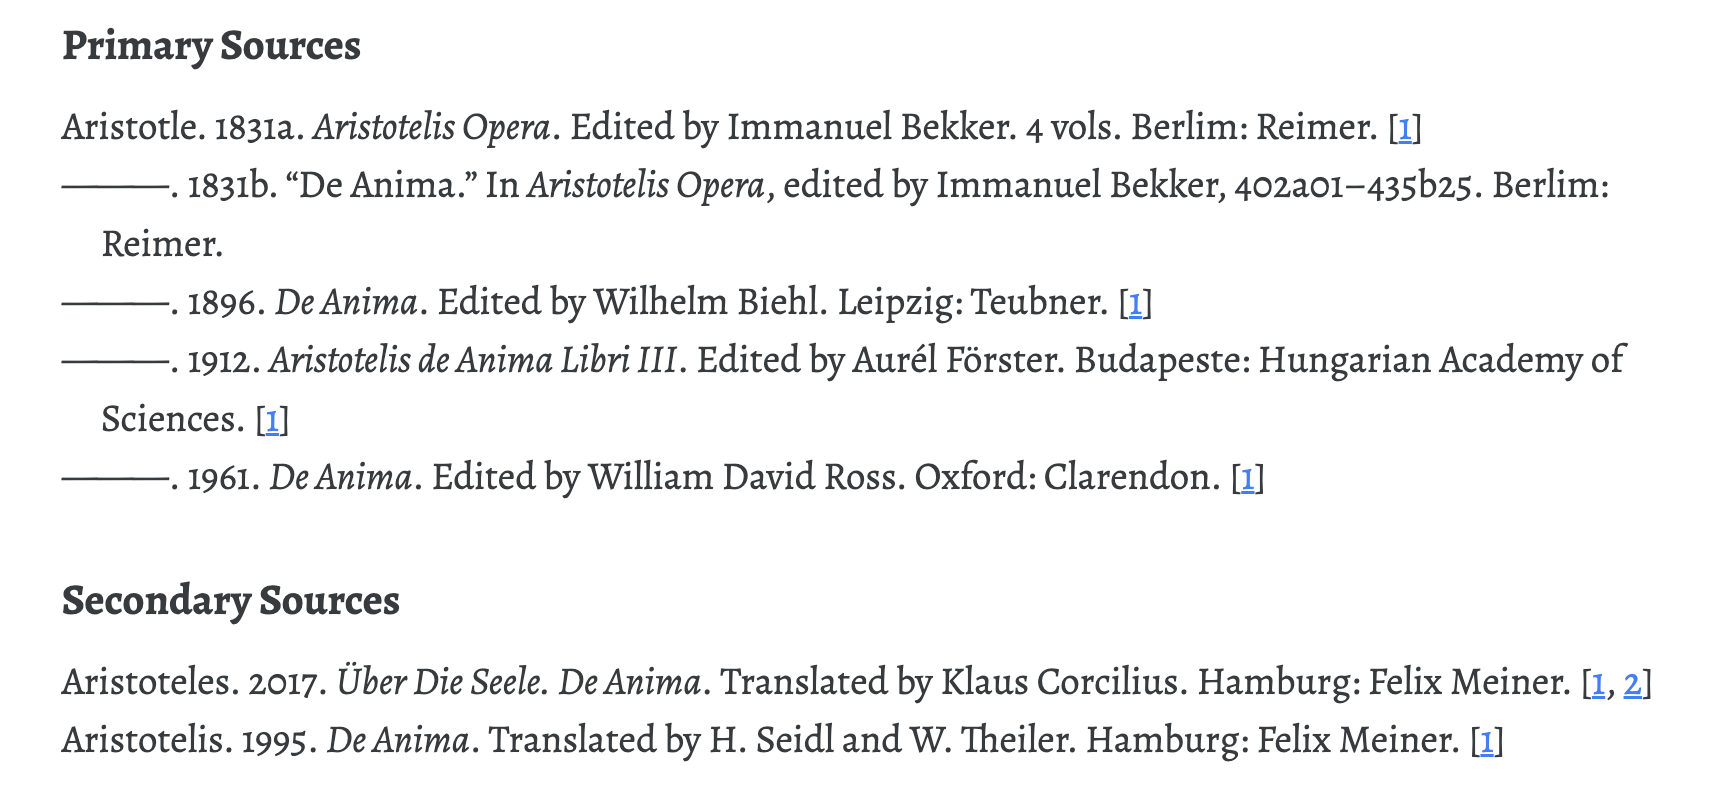
\includegraphics[width=4.70833in,height=2.15625in]{multipartbibliography.png}

}

\caption{\label{fig-scriv165A}Multipart bibliography with sections, such
as primary sources and secondary sources}

\end{figure}

\begin{figure}

{\centering 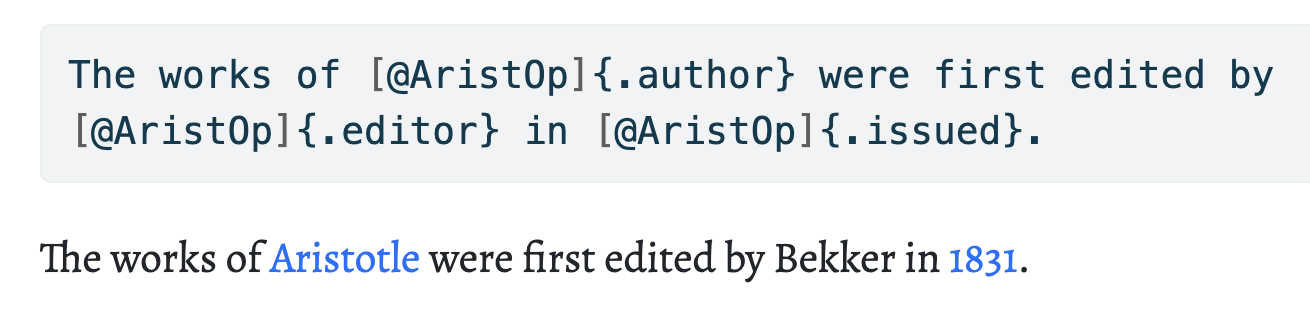
\includegraphics[width=4.75in,height=1.125in]{citefield.png}

}

\caption{\label{fig-scriv165B}Cite Field allows the evocation of
arbitrary information from the references, such as \texttt{author},
\texttt{editor}, \texttt{translator} (using
\href{https://docs.citationstyles.org/en/stable/specification.html\#appendix-iv-variables}{CSL
variables} name conventions)}

\end{figure}

\begin{figure}

{\centering 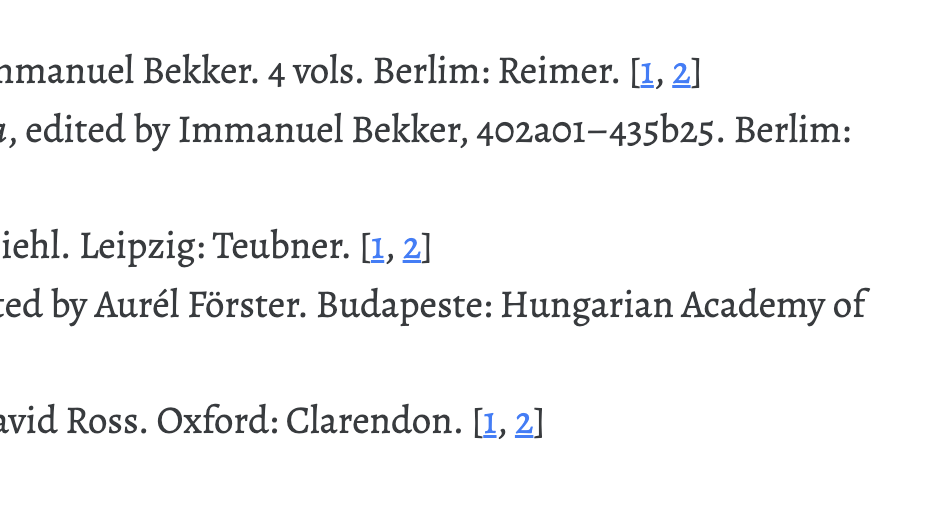
\includegraphics[width=4.84375in,height=2.6875in]{backrefs.png}

}

\caption{\label{fig-scriv165C}The \textbf{Citation Backlinks} filter
adds an index of cited references to the bibliography, with links back
to all in-text citations. It also allows the user to turn these off
globally or in an \emph{ad hoc} fashion.}

\end{figure}



\backmatter



\end{document}
